%! TEX encoding = utf8
\chapter{Laboratorium}

\section{Określenie wartości pomiaru temperatury w punkcie pracy}

W celu określenia wartości pomiaru temperatury w punkcie pracy ustawiono moc wentylatora  $W1 = 50\%$,a moc grzałki $G1 = 25\%$.
Po czasie około 8 minut temperatura odczytywana przez czujnik temperatury zaczeła się stabilizować  na poziomie  $T1 = 30,93^{\circ} C$.

Niestety z powodu ciągłego ruchu powietrza związanego z przemieszczaniem się osób w sali i dużej ilości tych osób wpływających na temperaturę sali oraz czułość stanowiska pomiarowego temperatura odczytywana przez czujnik zaczeła odbiegać i lekko oscylować wokół tej temperatury.

\begin{figure}[H]
\centering
% This file was created by matlab2tikz.
%
%The latest updates can be retrieved from
%  http://www.mathworks.com/matlabcentral/fileexchange/22022-matlab2tikz-matlab2tikz
%where you can also make suggestions and rate matlab2tikz.
%
\definecolor{mycolor1}{rgb}{0.00000,0.44700,0.74100}%
%
\begin{tikzpicture}

\begin{axis}[%
width=4.521in,
height=3.566in,
at={(0.758in,0.481in)},
scale only axis,
xmin=0,
xmax=450,
xlabel style={font=\color{white!15!black}},
xlabel={k},
ymin=25,
ymax=31,
ylabel style={font=\color{white!15!black}},
ylabel={$\text{T[}^\circ\text{C]}$},
axis background/.style={fill=white}
]
\addplot[const plot, color=mycolor1, forget plot] table[row sep=crcr] {%
1	25.12\\
2	25.12\\
3	25.18\\
4	25.25\\
5	25.37\\
6	25.43\\
7	25.5\\
8	25.62\\
9	25.68\\
10	25.75\\
11	25.81\\
12	25.87\\
13	26\\
14	26.06\\
15	26.12\\
16	26.18\\
17	26.25\\
18	26.31\\
19	26.43\\
20	26.5\\
21	26.56\\
22	26.62\\
23	26.68\\
24	26.68\\
25	26.81\\
26	26.81\\
27	26.87\\
28	26.93\\
29	27\\
30	27.06\\
31	27.12\\
32	27.18\\
33	27.18\\
34	27.25\\
35	27.31\\
36	27.37\\
37	27.37\\
38	27.43\\
39	27.5\\
40	27.5\\
41	27.56\\
42	27.62\\
43	27.62\\
44	27.68\\
45	27.68\\
46	27.75\\
47	27.81\\
48	27.81\\
49	27.87\\
50	27.87\\
51	27.93\\
52	28\\
53	28\\
54	28\\
55	28.06\\
56	28.06\\
57	28.12\\
58	28.12\\
59	28.18\\
60	28.18\\
61	28.25\\
62	28.25\\
63	28.25\\
64	28.31\\
65	28.37\\
66	28.37\\
67	28.37\\
68	28.43\\
69	28.43\\
70	28.5\\
71	28.5\\
72	28.5\\
73	28.56\\
74	28.56\\
75	28.56\\
76	28.62\\
77	28.62\\
78	28.68\\
79	28.68\\
80	28.68\\
81	28.75\\
82	28.75\\
83	28.81\\
84	28.81\\
85	28.81\\
86	28.87\\
87	28.87\\
88	28.93\\
89	28.93\\
90	29\\
91	29\\
92	29\\
93	29\\
94	29.06\\
95	29.06\\
96	29.06\\
97	29.12\\
98	29.12\\
99	29.12\\
100	29.12\\
101	29.18\\
102	29.18\\
103	29.18\\
104	29.25\\
105	29.25\\
106	29.25\\
107	29.25\\
108	29.31\\
109	29.31\\
110	29.31\\
111	29.31\\
112	29.37\\
113	29.31\\
114	29.37\\
115	29.37\\
116	29.37\\
117	29.43\\
118	29.43\\
119	29.43\\
120	29.5\\
121	29.5\\
122	29.5\\
123	29.5\\
124	29.5\\
125	29.56\\
126	29.56\\
127	29.56\\
128	29.56\\
129	29.56\\
130	29.56\\
131	29.62\\
132	29.62\\
133	29.62\\
134	29.62\\
135	29.62\\
136	29.62\\
137	29.62\\
138	29.62\\
139	29.68\\
140	29.68\\
141	29.68\\
142	29.68\\
143	29.75\\
144	29.75\\
145	29.75\\
146	29.75\\
147	29.75\\
148	29.75\\
149	29.75\\
150	29.75\\
151	29.75\\
152	29.75\\
153	29.75\\
154	29.81\\
155	29.81\\
156	29.81\\
157	29.81\\
158	29.81\\
159	29.81\\
160	29.81\\
161	29.87\\
162	29.87\\
163	29.87\\
164	29.87\\
165	29.87\\
166	29.87\\
167	29.93\\
168	29.93\\
169	29.93\\
170	29.93\\
171	29.93\\
172	29.93\\
173	29.93\\
174	29.93\\
175	30\\
176	29.93\\
177	30\\
178	30\\
179	30\\
180	30\\
181	30\\
182	30\\
183	30\\
184	30\\
185	30\\
186	30.06\\
187	30.06\\
188	30.06\\
189	30.06\\
190	30.06\\
191	30.06\\
192	30.06\\
193	30.06\\
194	30.06\\
195	30.06\\
196	30.06\\
197	30.06\\
198	30.06\\
199	30.06\\
200	30.06\\
201	30.06\\
202	30.12\\
203	30.12\\
204	30.12\\
205	30.12\\
206	30.12\\
207	30.12\\
208	30.12\\
209	30.18\\
210	30.18\\
211	30.18\\
212	30.18\\
213	30.18\\
214	30.18\\
215	30.18\\
216	30.18\\
217	30.18\\
218	30.25\\
219	30.25\\
220	30.25\\
221	30.25\\
222	30.25\\
223	30.25\\
224	30.25\\
225	30.31\\
226	30.25\\
227	30.25\\
228	30.31\\
229	30.31\\
230	30.25\\
231	30.31\\
232	30.31\\
233	30.31\\
234	30.31\\
235	30.31\\
236	30.31\\
237	30.31\\
238	30.31\\
239	30.31\\
240	30.31\\
241	30.31\\
242	30.37\\
243	30.37\\
244	30.37\\
245	30.37\\
246	30.37\\
247	30.43\\
248	30.43\\
249	30.43\\
250	30.43\\
251	30.43\\
252	30.43\\
253	30.43\\
254	30.43\\
255	30.43\\
256	30.5\\
257	30.5\\
258	30.5\\
259	30.5\\
260	30.5\\
261	30.56\\
262	30.56\\
263	30.56\\
264	30.56\\
265	30.56\\
266	30.62\\
267	30.56\\
268	30.62\\
269	30.56\\
270	30.56\\
271	30.56\\
272	30.56\\
273	30.56\\
274	30.56\\
275	30.56\\
276	30.56\\
277	30.56\\
278	30.56\\
279	30.56\\
280	30.56\\
281	30.56\\
282	30.56\\
283	30.56\\
284	30.56\\
285	30.56\\
286	30.56\\
287	30.62\\
288	30.62\\
289	30.56\\
290	30.56\\
291	30.62\\
292	30.62\\
293	30.62\\
294	30.62\\
295	30.62\\
296	30.62\\
297	30.62\\
298	30.62\\
299	30.62\\
300	30.62\\
301	30.62\\
302	30.62\\
303	30.62\\
304	30.62\\
305	30.62\\
306	30.62\\
307	30.62\\
308	30.62\\
309	30.62\\
310	30.62\\
311	30.68\\
312	30.68\\
313	30.62\\
314	30.68\\
315	30.68\\
316	30.68\\
317	30.68\\
318	30.68\\
319	30.68\\
320	30.68\\
321	30.68\\
322	30.68\\
323	30.68\\
324	30.68\\
325	30.68\\
326	30.68\\
327	30.68\\
328	30.68\\
329	30.68\\
330	30.68\\
331	30.68\\
332	30.68\\
333	30.68\\
334	30.68\\
335	30.68\\
336	30.68\\
337	30.68\\
338	30.68\\
339	30.68\\
340	30.68\\
341	30.68\\
342	30.68\\
343	30.68\\
344	30.68\\
345	30.75\\
346	30.75\\
347	30.75\\
348	30.75\\
349	30.75\\
350	30.75\\
351	30.75\\
352	30.81\\
353	30.75\\
354	30.75\\
355	30.81\\
356	30.75\\
357	30.81\\
358	30.81\\
359	30.81\\
360	30.81\\
361	30.81\\
362	30.81\\
363	30.81\\
364	30.75\\
365	30.81\\
366	30.75\\
367	30.81\\
368	30.81\\
369	30.81\\
370	30.81\\
371	30.81\\
372	30.81\\
373	30.81\\
374	30.81\\
375	30.81\\
376	30.87\\
377	30.87\\
378	30.87\\
379	30.87\\
380	30.87\\
381	30.93\\
382	30.93\\
383	30.93\\
384	30.93\\
385	30.93\\
386	30.93\\
387	30.93\\
388	30.93\\
389	30.93\\
390	30.93\\
391	30.93\\
392	30.87\\
393	30.87\\
394	30.87\\
395	30.87\\
396	30.87\\
397	30.87\\
398	30.87\\
399	30.87\\
400	30.87\\
401	30.87\\
402	30.87\\
403	30.87\\
404	30.87\\
405	30.87\\
406	30.87\\
407	30.87\\
408	30.87\\
409	30.87\\
410	30.87\\
411	30.87\\
412	30.87\\
413	30.87\\
414	30.87\\
415	30.87\\
416	30.87\\
417	30.87\\
418	30.87\\
419	30.87\\
420	30.93\\
421	30.93\\
422	30.93\\
423	30.93\\
424	30.93\\
425	30.93\\
426	30.87\\
427	30.93\\
428	30.93\\
429	30.87\\
430	30.93\\
431	30.93\\
432	30.93\\
433	30.93\\
434	30.93\\
435	30.93\\
436	30.93\\
437	30.93\\
438	30.93\\
439	30.93\\
440	30.93\\
441	30.93\\
442	30.93\\
443	30.93\\
444	31\\
445	30.93\\
446	30.93\\
447	30.93\\
448	30.93\\
449	30.93\\
450	30.93\\
};
\end{axis}
\end{tikzpicture}%
\caption{Pomiar temperatury w punkcie pracy}
\end{figure}

\section{Wyznaczenie odpowiedzi skokowych}

Doprowadziliśmy układ do stanu stabilnego dla 7 różnych wartości sterowania: $U = 20$, $U = 30$, $U = 40$, $U = 50$, $U = 60$, $U = 70$, $U = 80$.

\begin{figure}[H]
\centering
% This file was created by matlab2tikz.
%
%The latest updates can be retrieved from
%  http://www.mathworks.com/matlabcentral/fileexchange/22022-matlab2tikz-matlab2tikz
%where you can also make suggestions and rate matlab2tikz.
%
\definecolor{mycolor1}{rgb}{0.00000,0.44700,0.74100}%
\definecolor{mycolor2}{rgb}{0.85000,0.32500,0.09800}%
\definecolor{mycolor3}{rgb}{0.92900,0.69400,0.12500}%
%
\begin{tikzpicture}

\begin{axis}[%
width=4.521in,
height=3.566in,
at={(0.758in,0.481in)},
scale only axis,
xmin=0,
xmax=350,
xlabel style={font=\color{white!15!black}},
xlabel={k},
ymin=28,
ymax=34,
ylabel style={font=\color{white!15!black}},
ylabel={$\text{T[}^\circ\text{C]}$},
axis background/.style={fill=white}
]
\addplot[const plot, color=mycolor1, forget plot] table[row sep=crcr] {%
1	28.18\\
2	28.18\\
3	28.18\\
4	28.18\\
5	28.12\\
6	28.12\\
7	28.12\\
8	28.12\\
9	28.12\\
10	28.12\\
11	28.12\\
12	28.12\\
13	28.06\\
14	28.12\\
15	28.12\\
16	28.12\\
17	28.12\\
18	28.18\\
19	28.18\\
20	28.18\\
21	28.18\\
22	28.25\\
23	28.25\\
24	28.25\\
25	28.25\\
26	28.31\\
27	28.31\\
28	28.31\\
29	28.37\\
30	28.37\\
31	28.43\\
32	28.43\\
33	28.43\\
34	28.5\\
35	28.56\\
36	28.56\\
37	28.62\\
38	28.62\\
39	28.68\\
40	28.68\\
41	28.68\\
42	28.75\\
43	28.75\\
44	28.81\\
45	28.87\\
46	28.87\\
47	28.87\\
48	28.93\\
49	28.93\\
50	29\\
51	29.06\\
52	29.06\\
53	29.12\\
54	29.18\\
55	29.18\\
56	29.25\\
57	29.25\\
58	29.31\\
59	29.31\\
60	29.37\\
61	29.37\\
62	29.37\\
63	29.37\\
64	29.43\\
65	29.43\\
66	29.5\\
67	29.5\\
68	29.5\\
69	29.56\\
70	29.56\\
71	29.56\\
72	29.62\\
73	29.62\\
74	29.62\\
75	29.62\\
76	29.62\\
77	29.62\\
78	29.62\\
79	29.62\\
80	29.62\\
81	29.62\\
82	29.62\\
83	29.62\\
84	29.62\\
85	29.62\\
86	29.62\\
87	29.62\\
88	29.62\\
89	29.68\\
90	29.68\\
91	29.68\\
92	29.68\\
93	29.75\\
94	29.75\\
95	29.75\\
96	29.75\\
97	29.81\\
98	29.81\\
99	29.81\\
100	29.81\\
101	29.81\\
102	29.81\\
103	29.87\\
104	29.87\\
105	29.87\\
106	29.87\\
107	29.87\\
108	29.87\\
109	29.87\\
110	29.93\\
111	29.93\\
112	29.87\\
113	29.87\\
114	29.87\\
115	29.87\\
116	29.93\\
117	29.87\\
118	29.93\\
119	29.93\\
120	29.93\\
121	29.93\\
122	29.93\\
123	29.93\\
124	29.93\\
125	29.87\\
126	29.87\\
127	29.93\\
128	29.93\\
129	29.93\\
130	29.93\\
131	29.93\\
132	29.93\\
133	30\\
134	30\\
135	30\\
136	30\\
137	30\\
138	30\\
139	30\\
140	30\\
141	30\\
142	30.06\\
143	30.06\\
144	30.06\\
145	30.06\\
146	30.06\\
147	30.12\\
148	30.12\\
149	30.12\\
150	30.12\\
151	30.12\\
152	30.12\\
153	30.12\\
154	30.12\\
155	30.12\\
156	30.18\\
157	30.18\\
158	30.18\\
159	30.18\\
160	30.18\\
161	30.18\\
162	30.25\\
163	30.25\\
164	30.25\\
165	30.25\\
166	30.25\\
167	30.25\\
168	30.31\\
169	30.31\\
170	30.31\\
171	30.31\\
172	30.31\\
173	30.31\\
174	30.37\\
175	30.37\\
176	30.37\\
177	30.37\\
178	30.37\\
179	30.37\\
180	30.43\\
181	30.43\\
182	30.43\\
183	30.43\\
184	30.43\\
185	30.43\\
186	30.43\\
187	30.37\\
188	30.43\\
189	30.37\\
190	30.37\\
191	30.37\\
192	30.37\\
193	30.37\\
194	30.37\\
195	30.37\\
196	30.37\\
197	30.37\\
198	30.37\\
199	30.37\\
200	30.37\\
201	30.37\\
202	30.37\\
203	30.37\\
204	30.37\\
205	30.37\\
206	30.37\\
207	30.37\\
208	30.37\\
209	30.37\\
210	30.37\\
211	30.37\\
212	30.37\\
213	30.37\\
214	30.37\\
215	30.37\\
216	30.37\\
217	30.37\\
218	30.37\\
219	30.37\\
220	30.43\\
221	30.43\\
222	30.43\\
223	30.43\\
224	30.43\\
225	30.43\\
226	30.43\\
227	30.43\\
228	30.43\\
229	30.43\\
230	30.43\\
231	30.43\\
232	30.43\\
233	30.37\\
234	30.37\\
235	30.37\\
236	30.37\\
237	30.43\\
238	30.43\\
239	30.43\\
240	30.43\\
241	30.43\\
242	30.43\\
243	30.43\\
244	30.43\\
245	30.43\\
246	30.43\\
247	30.43\\
248	30.5\\
249	30.5\\
250	30.5\\
251	30.5\\
252	30.5\\
253	30.5\\
254	30.5\\
255	30.5\\
256	30.5\\
257	30.5\\
258	30.5\\
259	30.5\\
260	30.5\\
261	30.5\\
262	30.5\\
263	30.5\\
264	30.5\\
265	30.56\\
266	30.5\\
267	30.5\\
268	30.5\\
269	30.5\\
270	30.5\\
271	30.5\\
272	30.5\\
273	30.5\\
274	30.5\\
275	30.5\\
276	30.5\\
277	30.5\\
278	30.5\\
279	30.5\\
280	30.5\\
281	30.5\\
282	30.5\\
283	30.5\\
284	30.5\\
285	30.5\\
286	30.5\\
287	30.56\\
288	30.56\\
289	30.56\\
290	30.56\\
291	30.56\\
292	30.56\\
293	30.56\\
294	30.56\\
295	30.56\\
296	30.56\\
297	30.56\\
298	30.56\\
299	30.56\\
300	30.56\\
301	30.5\\
302	30.5\\
303	30.5\\
304	30.5\\
305	30.5\\
306	30.5\\
307	30.43\\
308	30.43\\
309	30.43\\
310	30.43\\
311	30.43\\
312	30.43\\
313	30.43\\
314	30.43\\
315	30.37\\
316	30.37\\
317	30.37\\
318	30.37\\
319	30.37\\
320	30.37\\
321	30.37\\
322	30.37\\
323	30.37\\
324	30.37\\
325	30.37\\
326	30.43\\
327	30.43\\
328	30.43\\
329	30.5\\
330	30.43\\
331	30.5\\
332	30.5\\
333	30.5\\
334	30.56\\
335	30.56\\
336	30.56\\
337	30.56\\
338	30.56\\
339	30.56\\
340	30.56\\
341	30.56\\
342	30.62\\
343	30.62\\
344	30.62\\
345	30.62\\
346	30.62\\
347	30.62\\
348	30.62\\
349	30.62\\
350	30.62\\
};
\addplot[const plot, color=mycolor2, forget plot] table[row sep=crcr] {%
1	28.12\\
2	28.18\\
3	28.18\\
4	28.18\\
5	28.18\\
6	28.18\\
7	28.18\\
8	28.18\\
9	28.18\\
10	28.18\\
11	28.18\\
12	28.18\\
13	28.18\\
14	28.18\\
15	28.18\\
16	28.18\\
17	28.18\\
18	28.18\\
19	28.18\\
20	28.25\\
21	28.25\\
22	28.25\\
23	28.31\\
24	28.31\\
25	28.31\\
26	28.37\\
27	28.37\\
28	28.43\\
29	28.5\\
30	28.5\\
31	28.56\\
32	28.56\\
33	28.62\\
34	28.62\\
35	28.68\\
36	28.75\\
37	28.81\\
38	28.81\\
39	28.87\\
40	28.93\\
41	28.93\\
42	29\\
43	29.06\\
44	29.06\\
45	29.06\\
46	29.12\\
47	29.18\\
48	29.18\\
49	29.25\\
50	29.31\\
51	29.31\\
52	29.31\\
53	29.37\\
54	29.43\\
55	29.43\\
56	29.5\\
57	29.5\\
58	29.56\\
59	29.62\\
60	29.62\\
61	29.68\\
62	29.68\\
63	29.75\\
64	29.75\\
65	29.81\\
66	29.81\\
67	29.81\\
68	29.87\\
69	29.87\\
70	29.93\\
71	29.93\\
72	30\\
73	30\\
74	30.06\\
75	30.06\\
76	30.12\\
77	30.12\\
78	30.18\\
79	30.18\\
80	30.18\\
81	30.25\\
82	30.31\\
83	30.31\\
84	30.31\\
85	30.37\\
86	30.37\\
87	30.37\\
88	30.37\\
89	30.43\\
90	30.43\\
91	30.43\\
92	30.43\\
93	30.43\\
94	30.5\\
95	30.5\\
96	30.5\\
97	30.5\\
98	30.5\\
99	30.56\\
100	30.62\\
101	30.62\\
102	30.62\\
103	30.62\\
104	30.68\\
105	30.68\\
106	30.75\\
107	30.75\\
108	30.81\\
109	30.81\\
110	30.87\\
111	30.87\\
112	30.87\\
113	30.93\\
114	30.93\\
115	31\\
116	31\\
117	31.06\\
118	31\\
119	31.06\\
120	31.06\\
121	31\\
122	31\\
123	31\\
124	31.06\\
125	31\\
126	31\\
127	31.06\\
128	31.06\\
129	31.06\\
130	31.06\\
131	31.06\\
132	31.12\\
133	31.12\\
134	31.12\\
135	31.12\\
136	31.18\\
137	31.18\\
138	31.18\\
139	31.18\\
140	31.18\\
141	31.18\\
142	31.25\\
143	31.25\\
144	31.25\\
145	31.25\\
146	31.25\\
147	31.31\\
148	31.31\\
149	31.31\\
150	31.31\\
151	31.31\\
152	31.37\\
153	31.37\\
154	31.37\\
155	31.43\\
156	31.43\\
157	31.5\\
158	31.5\\
159	31.5\\
160	31.5\\
161	31.5\\
162	31.5\\
163	31.5\\
164	31.5\\
165	31.56\\
166	31.56\\
167	31.56\\
168	31.56\\
169	31.56\\
170	31.56\\
171	31.56\\
172	31.56\\
173	31.62\\
174	31.62\\
175	31.62\\
176	31.62\\
177	31.62\\
178	31.68\\
179	31.68\\
180	31.68\\
181	31.62\\
182	31.68\\
183	31.68\\
184	31.68\\
185	31.68\\
186	31.68\\
187	31.68\\
188	31.68\\
189	31.68\\
190	31.68\\
191	31.62\\
192	31.62\\
193	31.68\\
194	31.68\\
195	31.68\\
196	31.68\\
197	31.68\\
198	31.68\\
199	31.68\\
200	31.68\\
201	31.68\\
202	31.68\\
203	31.62\\
204	31.68\\
205	31.68\\
206	31.68\\
207	31.68\\
208	31.68\\
209	31.68\\
210	31.75\\
211	31.75\\
212	31.75\\
213	31.75\\
214	31.75\\
215	31.75\\
216	31.81\\
217	31.81\\
218	31.81\\
219	31.81\\
220	31.81\\
221	31.81\\
222	31.87\\
223	31.87\\
224	31.87\\
225	31.87\\
226	31.87\\
227	31.93\\
228	31.93\\
229	31.93\\
230	31.93\\
231	32\\
232	32\\
233	32\\
234	32\\
235	32\\
236	32\\
237	32\\
238	32\\
239	32\\
240	32\\
241	32\\
242	32\\
243	32\\
244	32.06\\
245	32.06\\
246	32.06\\
247	32.06\\
248	32.06\\
249	32.06\\
250	32.06\\
251	32.06\\
252	32\\
253	32\\
254	32\\
255	32\\
256	32\\
257	32\\
258	32\\
259	32\\
260	32\\
261	32\\
262	32\\
263	32\\
264	32\\
265	31.93\\
266	32\\
267	32\\
268	32\\
269	32\\
270	32\\
271	32\\
272	32\\
273	31.93\\
274	31.93\\
275	32\\
276	31.93\\
277	31.93\\
278	31.93\\
279	31.93\\
280	31.93\\
281	31.93\\
282	31.93\\
283	31.93\\
284	32\\
285	32\\
286	32\\
287	32\\
288	32\\
289	32\\
290	32\\
291	32\\
292	32\\
293	32\\
294	32\\
295	32\\
296	32\\
297	32\\
298	32\\
299	32\\
300	32\\
301	32.06\\
302	32\\
303	32\\
304	32\\
305	32.06\\
306	32.06\\
307	32.06\\
308	32.06\\
309	32.12\\
310	32.12\\
311	32.12\\
312	32.12\\
313	32.12\\
314	32.18\\
315	32.18\\
316	32.18\\
317	32.18\\
318	32.18\\
319	32.25\\
320	32.18\\
321	32.25\\
322	32.25\\
323	32.25\\
324	32.25\\
325	32.25\\
326	32.25\\
327	32.25\\
328	32.25\\
329	32.25\\
330	32.25\\
331	32.18\\
332	32.18\\
333	32.25\\
334	32.25\\
335	32.25\\
336	32.25\\
337	32.25\\
338	32.25\\
339	32.25\\
340	32.31\\
341	32.31\\
342	32.31\\
343	32.31\\
344	32.31\\
345	32.25\\
346	32.25\\
347	32.31\\
348	32.31\\
349	32.31\\
350	32.31\\
};
\addplot[const plot, color=mycolor3, forget plot] table[row sep=crcr] {%
1	28.18\\
2	28.18\\
3	28.18\\
4	28.25\\
5	28.25\\
6	28.25\\
7	28.25\\
8	28.25\\
9	28.31\\
10	28.25\\
11	28.25\\
12	28.25\\
13	28.25\\
14	28.25\\
15	28.25\\
16	28.25\\
17	28.25\\
18	28.31\\
19	28.31\\
20	28.31\\
21	28.37\\
22	28.37\\
23	28.43\\
24	28.43\\
25	28.5\\
26	28.5\\
27	28.56\\
28	28.62\\
29	28.62\\
30	28.68\\
31	28.75\\
32	28.81\\
33	28.87\\
34	28.87\\
35	28.93\\
36	29\\
37	29.06\\
38	29.12\\
39	29.25\\
40	29.31\\
41	29.37\\
42	29.43\\
43	29.5\\
44	29.56\\
45	29.62\\
46	29.68\\
47	29.75\\
48	29.81\\
49	29.87\\
50	29.93\\
51	30\\
52	30.06\\
53	30.12\\
54	30.18\\
55	30.25\\
56	30.31\\
57	30.31\\
58	30.37\\
59	30.43\\
60	30.5\\
61	30.5\\
62	30.5\\
63	30.56\\
64	30.62\\
65	30.68\\
66	30.75\\
67	30.75\\
68	30.81\\
69	30.87\\
70	30.87\\
71	30.93\\
72	31\\
73	31\\
74	31.06\\
75	31.12\\
76	31.12\\
77	31.18\\
78	31.18\\
79	31.25\\
80	31.25\\
81	31.31\\
82	31.37\\
83	31.37\\
84	31.43\\
85	31.5\\
86	31.5\\
87	31.56\\
88	31.62\\
89	31.62\\
90	31.68\\
91	31.68\\
92	31.68\\
93	31.75\\
94	31.75\\
95	31.81\\
96	31.81\\
97	31.81\\
98	31.87\\
99	31.93\\
100	31.93\\
101	31.93\\
102	32\\
103	32.06\\
104	32.06\\
105	32.12\\
106	32.12\\
107	32.18\\
108	32.18\\
109	32.25\\
110	32.25\\
111	32.25\\
112	32.25\\
113	32.31\\
114	32.31\\
115	32.37\\
116	32.37\\
117	32.37\\
118	32.37\\
119	32.43\\
120	32.43\\
121	32.43\\
122	32.43\\
123	32.43\\
124	32.43\\
125	32.43\\
126	32.43\\
127	32.5\\
128	32.5\\
129	32.5\\
130	32.56\\
131	32.56\\
132	32.56\\
133	32.62\\
134	32.62\\
135	32.62\\
136	32.62\\
137	32.62\\
138	32.62\\
139	32.62\\
140	32.62\\
141	32.62\\
142	32.62\\
143	32.68\\
144	32.68\\
145	32.68\\
146	32.68\\
147	32.68\\
148	32.68\\
149	32.75\\
150	32.68\\
151	32.75\\
152	32.75\\
153	32.75\\
154	32.75\\
155	32.75\\
156	32.75\\
157	32.81\\
158	32.81\\
159	32.81\\
160	32.87\\
161	32.87\\
162	32.87\\
163	32.87\\
164	32.93\\
165	32.93\\
166	32.93\\
167	32.93\\
168	32.93\\
169	33\\
170	33\\
171	33.06\\
172	33.06\\
173	33.06\\
174	33.06\\
175	33.06\\
176	33.12\\
177	33.12\\
178	33.18\\
179	33.18\\
180	33.25\\
181	33.25\\
182	33.25\\
183	33.25\\
184	33.31\\
185	33.31\\
186	33.31\\
187	33.31\\
188	33.37\\
189	33.37\\
190	33.37\\
191	33.43\\
192	33.43\\
193	33.43\\
194	33.43\\
195	33.43\\
196	33.5\\
197	33.5\\
198	33.5\\
199	33.5\\
200	33.5\\
201	33.5\\
202	33.5\\
203	33.5\\
204	33.5\\
205	33.5\\
206	33.5\\
207	33.5\\
208	33.5\\
209	33.5\\
210	33.5\\
211	33.5\\
212	33.5\\
213	33.5\\
214	33.5\\
215	33.5\\
216	33.5\\
217	33.5\\
218	33.56\\
219	33.56\\
220	33.56\\
221	33.56\\
222	33.56\\
223	33.56\\
224	33.62\\
225	33.62\\
226	33.62\\
227	33.62\\
228	33.62\\
229	33.62\\
230	33.62\\
231	33.62\\
232	33.62\\
233	33.62\\
234	33.68\\
235	33.68\\
236	33.62\\
237	33.68\\
238	33.68\\
239	33.62\\
240	33.62\\
241	33.62\\
242	33.62\\
243	33.62\\
244	33.56\\
245	33.62\\
246	33.56\\
247	33.56\\
248	33.56\\
249	33.62\\
250	33.56\\
251	33.62\\
252	33.62\\
253	33.68\\
254	33.68\\
255	33.75\\
256	33.81\\
257	33.81\\
258	33.81\\
259	33.81\\
260	33.87\\
261	33.87\\
262	33.87\\
263	33.87\\
264	33.87\\
265	33.87\\
266	33.87\\
267	33.87\\
268	33.87\\
269	33.87\\
270	33.93\\
271	33.93\\
272	33.87\\
273	33.93\\
274	33.93\\
275	33.93\\
276	33.93\\
277	33.93\\
278	33.93\\
279	33.93\\
280	33.93\\
281	33.93\\
282	33.93\\
283	33.93\\
284	33.93\\
285	33.93\\
286	33.93\\
287	33.93\\
288	33.93\\
289	33.87\\
290	33.87\\
291	33.93\\
292	33.87\\
293	33.87\\
294	33.87\\
295	33.87\\
296	33.87\\
297	33.87\\
298	33.87\\
299	33.87\\
300	33.87\\
301	33.87\\
302	33.87\\
303	33.87\\
304	33.87\\
305	33.87\\
306	33.87\\
307	33.87\\
308	33.87\\
309	33.87\\
310	33.87\\
311	33.87\\
312	33.87\\
313	33.93\\
314	33.93\\
315	33.93\\
316	33.93\\
317	33.93\\
318	33.93\\
319	33.93\\
320	34\\
321	33.93\\
322	34\\
323	34\\
324	34\\
325	34\\
326	34\\
327	34\\
328	34\\
329	34\\
330	34\\
331	34\\
332	34\\
333	34\\
334	33.93\\
335	33.93\\
336	33.93\\
337	34\\
338	34\\
339	34\\
340	34\\
341	34\\
342	33.93\\
343	33.93\\
344	33.93\\
345	33.93\\
346	33.93\\
347	33.93\\
348	33.87\\
349	33.93\\
350	33.87\\
};
\end{axis}
\end{tikzpicture}%
\caption{Przebiegi wyjścia dla różnych sterowań}
\end{figure}

Analizując otrzymane wykresy można wywnioskować, że właściwości statyczne procesu jeżeli i są w przybliżeniu liniowe, to tylko w pewnych zakresach. Zmiany wartości odpowiedzi skokowej dla tych samych chwil są w przybliżeniu proporcjonalne dla pierwszych trzech sterowań oraz dla trzech ostatnich, ale to w przybliżeniu i ogólnie własności statyczne nie są liniowe.

W celu sprawdzenia założeń narysowano charakterystykę statyczną procesu.

\begin{figure}[H]
\centering
% This file was created by matlab2tikz.
%
%The latest updates can be retrieved from
%  http://www.mathworks.com/matlabcentral/fileexchange/22022-matlab2tikz-matlab2tikz
%where you can also make suggestions and rate matlab2tikz.
%
\definecolor{mycolor1}{rgb}{0.00000,0.44700,0.74100}%
%
\begin{tikzpicture}

\begin{axis}[%
width=6.028in,
height=4.754in,
at={(1.011in,0.642in)},
scale only axis,
xmin=20,
xmax=80,
xlabel style={font=\color{white!15!black}},
xlabel={U},
ymin=25,
ymax=50,
ylabel style={font=\color{white!15!black}},
ylabel={Y},
axis background/.style={fill=white}
]
\addplot [color=mycolor1, forget plot]
  table[row sep=crcr]{%
20	29.18\\
30	33.31\\
40	37.31\\
50	41.68\\
60	44.31\\
70	47.18\\
80	48.87\\
};
\end{axis}
\end{tikzpicture}%
\caption{Charakterystyka statyczna procesu}
\end{figure}

Która potwierdziła przypuszczenia, na jej podstawie można stwierdzić, że właściwości statyczne procesu nie są liniowe, a więc nie da się wyliczyć wzmocnienia statycznego.

\section{Testowanie regulatorów z laboratorium 1}

\subsection{PID z laboratorium 1}

W danym podejściu wykorzystaliśmy PID z laboratorium pierwszego, ale w celu stabilizacji regulacji obniżyliśmy wzmocnienie z wartości $K = 30$ do wartości $k = 25$.

Parametry regulatora:

\begin{equation}
K = 30; 
T_i = 35; 
T_d = 4,5; 
\end{equation}

Wyniki działania regulacji:

\begin{figure}[H]
\centering
% This file was created by matlab2tikz.
%
%The latest updates can be retrieved from
%  http://www.mathworks.com/matlabcentral/fileexchange/22022-matlab2tikz-matlab2tikz
%where you can also make suggestions and rate matlab2tikz.
%
\definecolor{mycolor1}{rgb}{0.00000,0.44700,0.74100}%
\definecolor{mycolor2}{rgb}{0.85000,0.32500,0.09800}%
%
\begin{tikzpicture}

\begin{axis}[%
width=4.521in,
height=3.566in,
at={(0.758in,0.481in)},
scale only axis,
xmin=0,
xmax=800,
xlabel style={font=\color{white!15!black}},
xlabel={k},
ymin=30,
ymax=48,
ylabel style={font=\color{white!15!black}},
ylabel={$\text{T[}^\circ\text{C]}$},
axis background/.style={fill=white},
legend style={legend cell align=left, align=left, draw=white!15!black}
]
\addplot[const plot, color=mycolor1] table[row sep=crcr] {%
1	31.18\\
2	31.18\\
3	31.25\\
4	31.25\\
5	31.31\\
6	31.31\\
7	31.31\\
8	31.37\\
9	31.37\\
10	31.43\\
11	31.43\\
12	31.43\\
13	31.43\\
14	31.43\\
15	31.43\\
16	31.5\\
17	31.43\\
18	31.43\\
19	31.43\\
20	31.43\\
21	31.43\\
22	31.43\\
23	31.37\\
24	31.37\\
25	31.37\\
26	31.31\\
27	31.31\\
28	31.31\\
29	31.25\\
30	31.25\\
31	31.18\\
32	31.18\\
33	31.18\\
34	31.18\\
35	31.12\\
36	31.12\\
37	31.12\\
38	31.12\\
39	31.06\\
40	31.06\\
41	31\\
42	31\\
43	31\\
44	31\\
45	31\\
46	31\\
47	30.93\\
48	30.93\\
49	30.93\\
50	30.93\\
51	30.93\\
52	30.93\\
53	30.93\\
54	30.93\\
55	30.93\\
56	30.93\\
57	30.93\\
58	31\\
59	31\\
60	31\\
61	31\\
62	31\\
63	30.93\\
64	31\\
65	30.93\\
66	30.93\\
67	30.93\\
68	30.87\\
69	30.93\\
70	30.93\\
71	30.93\\
72	30.93\\
73	31\\
74	31.06\\
75	31.12\\
76	31.18\\
77	31.25\\
78	31.37\\
79	31.43\\
80	31.56\\
81	31.68\\
82	31.81\\
83	31.93\\
84	32.06\\
85	32.18\\
86	32.31\\
87	32.5\\
88	32.62\\
89	32.75\\
90	32.87\\
91	33.06\\
92	33.25\\
93	33.43\\
94	33.56\\
95	33.68\\
96	33.87\\
97	34\\
98	34.18\\
99	34.31\\
100	34.5\\
101	34.62\\
102	34.75\\
103	34.87\\
104	35\\
105	35.12\\
106	35.18\\
107	35.31\\
108	35.37\\
109	35.5\\
110	35.56\\
111	35.62\\
112	35.68\\
113	35.75\\
114	35.81\\
115	35.81\\
116	35.87\\
117	35.87\\
118	35.87\\
119	35.87\\
120	35.87\\
121	35.87\\
122	35.87\\
123	35.87\\
124	35.87\\
125	35.87\\
126	35.87\\
127	35.87\\
128	35.81\\
129	35.81\\
130	35.75\\
131	35.68\\
132	35.62\\
133	35.62\\
134	35.56\\
135	35.56\\
136	35.5\\
137	35.43\\
138	35.43\\
139	35.37\\
140	35.37\\
141	35.31\\
142	35.31\\
143	35.31\\
144	35.31\\
145	35.31\\
146	35.31\\
147	35.31\\
148	35.31\\
149	35.37\\
150	35.37\\
151	35.43\\
152	35.43\\
153	35.5\\
154	35.5\\
155	35.56\\
156	35.56\\
157	35.62\\
158	35.68\\
159	35.68\\
160	35.68\\
161	35.81\\
162	35.81\\
163	35.87\\
164	35.87\\
165	35.93\\
166	36\\
167	36\\
168	36\\
169	36.06\\
170	36.06\\
171	36.06\\
172	36.12\\
173	36.12\\
174	36.12\\
175	36.12\\
176	36.12\\
177	36.12\\
178	36.12\\
179	36.18\\
180	36.18\\
181	36.18\\
182	36.18\\
183	36.12\\
184	36.12\\
185	36.12\\
186	36.12\\
187	36.12\\
188	36.12\\
189	36.06\\
190	36.06\\
191	36\\
192	36\\
193	36\\
194	35.93\\
195	35.93\\
196	35.93\\
197	35.93\\
198	35.93\\
199	35.93\\
200	35.87\\
201	35.87\\
202	35.81\\
203	35.81\\
204	35.81\\
205	35.75\\
206	35.75\\
207	35.75\\
208	35.75\\
209	35.68\\
210	35.68\\
211	35.68\\
212	35.68\\
213	35.68\\
214	35.68\\
215	35.68\\
216	35.68\\
217	35.68\\
218	35.68\\
219	35.68\\
220	35.68\\
221	35.75\\
222	35.75\\
223	35.81\\
224	35.81\\
225	35.87\\
226	35.87\\
227	35.93\\
228	35.93\\
229	35.93\\
230	36\\
231	36\\
232	36\\
233	36\\
234	36.06\\
235	36.06\\
236	36.06\\
237	36.06\\
238	36.06\\
239	36.06\\
240	36.06\\
241	36.06\\
242	36.06\\
243	36.06\\
244	36.06\\
245	36.06\\
246	36\\
247	36\\
248	36\\
249	36\\
250	36\\
251	36\\
252	35.93\\
253	35.93\\
254	35.93\\
255	35.93\\
256	35.93\\
257	35.87\\
258	35.87\\
259	35.87\\
260	35.87\\
261	35.87\\
262	35.87\\
263	35.87\\
264	35.93\\
265	35.93\\
266	35.93\\
267	35.93\\
268	35.93\\
269	35.93\\
270	35.93\\
271	35.93\\
272	35.93\\
273	35.93\\
274	35.93\\
275	35.93\\
276	35.93\\
277	35.87\\
278	35.87\\
279	35.87\\
280	35.87\\
281	35.93\\
282	35.93\\
283	35.93\\
284	35.93\\
285	36\\
286	36\\
287	36\\
288	36\\
289	36\\
290	36\\
291	36\\
292	36\\
293	35.93\\
294	36\\
295	35.93\\
296	36\\
297	36\\
298	36\\
299	36\\
300	36\\
301	35.93\\
302	35.93\\
303	35.93\\
304	35.93\\
305	35.93\\
306	35.93\\
307	35.93\\
308	36\\
309	36\\
310	36\\
311	35.93\\
312	35.93\\
313	35.93\\
314	35.87\\
315	35.87\\
316	35.87\\
317	35.87\\
318	35.87\\
319	35.87\\
320	35.87\\
321	35.87\\
322	35.93\\
323	36\\
324	36\\
325	36.12\\
326	36.18\\
327	36.31\\
328	36.37\\
329	36.5\\
330	36.62\\
331	36.81\\
332	36.93\\
333	37.06\\
334	37.18\\
335	37.37\\
336	37.5\\
337	37.68\\
338	37.81\\
339	38\\
340	38.12\\
341	38.31\\
342	38.43\\
343	38.62\\
344	38.81\\
345	38.93\\
346	39.12\\
347	39.25\\
348	39.43\\
349	39.62\\
350	39.81\\
351	39.93\\
352	40.12\\
353	40.25\\
354	40.43\\
355	40.56\\
356	40.75\\
357	40.87\\
358	41\\
359	41.12\\
360	41.31\\
361	41.37\\
362	41.56\\
363	41.68\\
364	41.81\\
365	41.93\\
366	42.06\\
367	42.18\\
368	42.31\\
369	42.43\\
370	42.56\\
371	42.68\\
372	42.81\\
373	42.93\\
374	43.06\\
375	43.18\\
376	43.37\\
377	43.5\\
378	43.62\\
379	43.68\\
380	43.81\\
381	43.87\\
382	43.93\\
383	44\\
384	44.06\\
385	44.12\\
386	44.18\\
387	44.25\\
388	44.31\\
389	44.31\\
390	44.37\\
391	44.43\\
392	44.5\\
393	44.5\\
394	44.56\\
395	44.56\\
396	44.62\\
397	44.62\\
398	44.68\\
399	44.68\\
400	44.75\\
401	44.75\\
402	44.75\\
403	44.81\\
404	44.81\\
405	44.87\\
406	44.87\\
407	44.93\\
408	45\\
409	45.06\\
410	45.12\\
411	45.12\\
412	45.18\\
413	45.25\\
414	45.31\\
415	45.31\\
416	45.43\\
417	45.5\\
418	45.56\\
419	45.62\\
420	45.62\\
421	45.68\\
422	45.75\\
423	45.81\\
424	45.87\\
425	45.87\\
426	45.93\\
427	45.93\\
428	45.93\\
429	45.87\\
430	45.93\\
431	45.93\\
432	45.93\\
433	45.93\\
434	46\\
435	46\\
436	46\\
437	46\\
438	46\\
439	46\\
440	45.93\\
441	46\\
442	45.93\\
443	46\\
444	46\\
445	45.93\\
446	46\\
447	45.93\\
448	46\\
449	46\\
450	46\\
451	46\\
452	45.93\\
453	45.93\\
454	45.93\\
455	45.93\\
456	45.93\\
457	45.93\\
458	45.93\\
459	45.87\\
460	45.87\\
461	45.87\\
462	45.87\\
463	45.87\\
464	45.87\\
465	45.87\\
466	45.87\\
467	45.81\\
468	45.81\\
469	45.81\\
470	45.87\\
471	45.81\\
472	45.87\\
473	45.81\\
474	45.87\\
475	45.81\\
476	45.81\\
477	45.87\\
478	45.87\\
479	45.87\\
480	45.87\\
481	45.87\\
482	45.87\\
483	45.87\\
484	45.87\\
485	45.93\\
486	45.93\\
487	45.93\\
488	45.93\\
489	46\\
490	46\\
491	46\\
492	46\\
493	46\\
494	46\\
495	46\\
496	46\\
497	46\\
498	46\\
499	45.93\\
500	45.93\\
501	46\\
502	46\\
503	46\\
504	46\\
505	46\\
506	46\\
507	46\\
508	46\\
509	46\\
510	46\\
511	46\\
512	45.93\\
513	45.93\\
514	45.87\\
515	45.87\\
516	45.81\\
517	45.81\\
518	45.68\\
519	45.62\\
520	45.56\\
521	45.5\\
522	45.31\\
523	45.18\\
524	45\\
525	44.81\\
526	44.68\\
527	44.5\\
528	44.31\\
529	44.12\\
530	43.93\\
531	43.68\\
532	43.5\\
533	43.31\\
534	43.12\\
535	42.87\\
536	42.68\\
537	42.43\\
538	42.25\\
539	42\\
540	41.75\\
541	41.5\\
542	41.18\\
543	40.93\\
544	40.68\\
545	40.43\\
546	40.18\\
547	39.93\\
548	39.68\\
549	39.43\\
550	39.18\\
551	39\\
552	38.75\\
553	38.5\\
554	38.31\\
555	38.12\\
556	37.93\\
557	37.75\\
558	37.56\\
559	37.43\\
560	37.25\\
561	37.06\\
562	36.87\\
563	36.75\\
564	36.56\\
565	36.43\\
566	36.25\\
567	36.12\\
568	35.93\\
569	35.81\\
570	35.68\\
571	35.5\\
572	35.37\\
573	35.18\\
574	35.06\\
575	34.87\\
576	34.75\\
577	34.62\\
578	34.43\\
579	34.25\\
580	34.12\\
581	33.93\\
582	33.81\\
583	33.68\\
584	33.56\\
585	33.43\\
586	33.31\\
587	33.18\\
588	33.12\\
589	33\\
590	32.93\\
591	32.81\\
592	32.75\\
593	32.68\\
594	32.68\\
595	32.62\\
596	32.56\\
597	32.56\\
598	32.5\\
599	32.5\\
600	32.43\\
601	32.37\\
602	32.37\\
603	32.37\\
604	32.31\\
605	32.31\\
606	32.31\\
607	32.25\\
608	32.25\\
609	32.18\\
610	32.18\\
611	32.12\\
612	32.12\\
613	32.06\\
614	32.06\\
615	32\\
616	32\\
617	31.93\\
618	31.93\\
619	31.87\\
620	31.81\\
621	31.75\\
622	31.75\\
623	31.68\\
624	31.62\\
625	31.56\\
626	31.56\\
627	31.5\\
628	31.5\\
629	31.43\\
630	31.37\\
631	31.37\\
632	31.31\\
633	31.31\\
634	31.25\\
635	31.18\\
636	31.18\\
637	31.12\\
638	31.12\\
639	31.06\\
640	31.06\\
641	31\\
642	31\\
643	31\\
644	30.93\\
645	30.93\\
646	30.93\\
647	30.93\\
648	30.93\\
649	30.93\\
650	30.93\\
651	30.93\\
652	30.93\\
653	30.93\\
654	31\\
655	31\\
656	31\\
657	31\\
658	31\\
659	31\\
660	31.06\\
661	31.06\\
662	31.06\\
663	31.06\\
664	31.06\\
665	31.06\\
666	31.12\\
667	31.06\\
668	31.12\\
669	31.12\\
670	31.12\\
671	31.12\\
672	31.12\\
673	31.12\\
674	31.12\\
675	31.12\\
676	31.12\\
677	31.12\\
678	31.06\\
679	31.06\\
680	31.06\\
681	31.06\\
682	31\\
683	31\\
684	31\\
685	31\\
686	30.93\\
687	30.93\\
688	30.93\\
689	30.93\\
690	30.93\\
691	30.87\\
692	30.87\\
693	30.81\\
694	30.81\\
695	30.81\\
696	30.75\\
697	30.75\\
698	30.75\\
699	30.75\\
700	30.75\\
701	30.68\\
702	30.75\\
703	30.75\\
704	30.75\\
705	30.75\\
706	30.75\\
707	30.68\\
708	30.75\\
709	30.75\\
710	30.75\\
711	30.75\\
712	30.75\\
713	30.81\\
714	30.81\\
715	30.87\\
716	30.87\\
717	30.93\\
718	30.93\\
719	30.93\\
720	31\\
721	31\\
722	31.06\\
723	31.06\\
724	31.06\\
725	31.06\\
726	31.06\\
727	31.12\\
728	31.06\\
729	31.12\\
730	31.12\\
731	31.06\\
732	31.12\\
733	31.06\\
734	31.06\\
735	31.06\\
736	31.06\\
737	31\\
738	31\\
739	31\\
740	31\\
741	30.93\\
742	30.93\\
743	30.93\\
744	30.87\\
745	30.87\\
746	30.81\\
747	30.81\\
748	30.75\\
749	30.75\\
750	30.75\\
751	30.75\\
752	30.81\\
753	30.81\\
754	30.81\\
755	30.81\\
756	30.81\\
757	30.81\\
758	30.81\\
759	30.87\\
760	30.87\\
761	30.87\\
762	30.93\\
763	30.93\\
764	30.93\\
765	31\\
766	31\\
767	31\\
768	31.06\\
769	31\\
770	31.06\\
771	31.06\\
772	31.06\\
773	31.06\\
774	31.12\\
775	31.06\\
776	31.06\\
777	31.06\\
778	31.12\\
779	31.12\\
780	31.12\\
781	31.06\\
782	31.06\\
783	31.06\\
784	31\\
785	31\\
786	30.93\\
787	30.93\\
788	30.93\\
789	30.87\\
790	30.87\\
791	30.81\\
792	30.81\\
793	30.81\\
794	30.75\\
795	30.75\\
796	30.68\\
797	30.68\\
798	30.68\\
799	30.62\\
800	30.62\\
};
\addlegendentry{Y}

\addplot[const plot, color=mycolor2, dashed] table[row sep=crcr] {%
1	30.93\\
2	30.93\\
3	30.93\\
4	30.93\\
5	30.93\\
6	30.93\\
7	30.93\\
8	30.93\\
9	30.93\\
10	30.93\\
11	30.93\\
12	30.93\\
13	30.93\\
14	30.93\\
15	30.93\\
16	30.93\\
17	30.93\\
18	30.93\\
19	30.93\\
20	30.93\\
21	30.93\\
22	30.93\\
23	30.93\\
24	30.93\\
25	30.93\\
26	30.93\\
27	30.93\\
28	30.93\\
29	30.93\\
30	30.93\\
31	30.93\\
32	30.93\\
33	30.93\\
34	30.93\\
35	30.93\\
36	30.93\\
37	30.93\\
38	30.93\\
39	30.93\\
40	30.93\\
41	30.93\\
42	30.93\\
43	30.93\\
44	30.93\\
45	30.93\\
46	30.93\\
47	30.93\\
48	30.93\\
49	30.93\\
50	30.93\\
51	35.93\\
52	35.93\\
53	35.93\\
54	35.93\\
55	35.93\\
56	35.93\\
57	35.93\\
58	35.93\\
59	35.93\\
60	35.93\\
61	35.93\\
62	35.93\\
63	35.93\\
64	35.93\\
65	35.93\\
66	35.93\\
67	35.93\\
68	35.93\\
69	35.93\\
70	35.93\\
71	35.93\\
72	35.93\\
73	35.93\\
74	35.93\\
75	35.93\\
76	35.93\\
77	35.93\\
78	35.93\\
79	35.93\\
80	35.93\\
81	35.93\\
82	35.93\\
83	35.93\\
84	35.93\\
85	35.93\\
86	35.93\\
87	35.93\\
88	35.93\\
89	35.93\\
90	35.93\\
91	35.93\\
92	35.93\\
93	35.93\\
94	35.93\\
95	35.93\\
96	35.93\\
97	35.93\\
98	35.93\\
99	35.93\\
100	35.93\\
101	35.93\\
102	35.93\\
103	35.93\\
104	35.93\\
105	35.93\\
106	35.93\\
107	35.93\\
108	35.93\\
109	35.93\\
110	35.93\\
111	35.93\\
112	35.93\\
113	35.93\\
114	35.93\\
115	35.93\\
116	35.93\\
117	35.93\\
118	35.93\\
119	35.93\\
120	35.93\\
121	35.93\\
122	35.93\\
123	35.93\\
124	35.93\\
125	35.93\\
126	35.93\\
127	35.93\\
128	35.93\\
129	35.93\\
130	35.93\\
131	35.93\\
132	35.93\\
133	35.93\\
134	35.93\\
135	35.93\\
136	35.93\\
137	35.93\\
138	35.93\\
139	35.93\\
140	35.93\\
141	35.93\\
142	35.93\\
143	35.93\\
144	35.93\\
145	35.93\\
146	35.93\\
147	35.93\\
148	35.93\\
149	35.93\\
150	35.93\\
151	35.93\\
152	35.93\\
153	35.93\\
154	35.93\\
155	35.93\\
156	35.93\\
157	35.93\\
158	35.93\\
159	35.93\\
160	35.93\\
161	35.93\\
162	35.93\\
163	35.93\\
164	35.93\\
165	35.93\\
166	35.93\\
167	35.93\\
168	35.93\\
169	35.93\\
170	35.93\\
171	35.93\\
172	35.93\\
173	35.93\\
174	35.93\\
175	35.93\\
176	35.93\\
177	35.93\\
178	35.93\\
179	35.93\\
180	35.93\\
181	35.93\\
182	35.93\\
183	35.93\\
184	35.93\\
185	35.93\\
186	35.93\\
187	35.93\\
188	35.93\\
189	35.93\\
190	35.93\\
191	35.93\\
192	35.93\\
193	35.93\\
194	35.93\\
195	35.93\\
196	35.93\\
197	35.93\\
198	35.93\\
199	35.93\\
200	35.93\\
201	35.93\\
202	35.93\\
203	35.93\\
204	35.93\\
205	35.93\\
206	35.93\\
207	35.93\\
208	35.93\\
209	35.93\\
210	35.93\\
211	35.93\\
212	35.93\\
213	35.93\\
214	35.93\\
215	35.93\\
216	35.93\\
217	35.93\\
218	35.93\\
219	35.93\\
220	35.93\\
221	35.93\\
222	35.93\\
223	35.93\\
224	35.93\\
225	35.93\\
226	35.93\\
227	35.93\\
228	35.93\\
229	35.93\\
230	35.93\\
231	35.93\\
232	35.93\\
233	35.93\\
234	35.93\\
235	35.93\\
236	35.93\\
237	35.93\\
238	35.93\\
239	35.93\\
240	35.93\\
241	35.93\\
242	35.93\\
243	35.93\\
244	35.93\\
245	35.93\\
246	35.93\\
247	35.93\\
248	35.93\\
249	35.93\\
250	35.93\\
251	35.93\\
252	35.93\\
253	35.93\\
254	35.93\\
255	35.93\\
256	35.93\\
257	35.93\\
258	35.93\\
259	35.93\\
260	35.93\\
261	35.93\\
262	35.93\\
263	35.93\\
264	35.93\\
265	35.93\\
266	35.93\\
267	35.93\\
268	35.93\\
269	35.93\\
270	35.93\\
271	35.93\\
272	35.93\\
273	35.93\\
274	35.93\\
275	35.93\\
276	35.93\\
277	35.93\\
278	35.93\\
279	35.93\\
280	35.93\\
281	35.93\\
282	35.93\\
283	35.93\\
284	35.93\\
285	35.93\\
286	35.93\\
287	35.93\\
288	35.93\\
289	35.93\\
290	35.93\\
291	35.93\\
292	35.93\\
293	35.93\\
294	35.93\\
295	35.93\\
296	35.93\\
297	35.93\\
298	35.93\\
299	35.93\\
300	35.93\\
301	45.93\\
302	45.93\\
303	45.93\\
304	45.93\\
305	45.93\\
306	45.93\\
307	45.93\\
308	45.93\\
309	45.93\\
310	45.93\\
311	45.93\\
312	45.93\\
313	45.93\\
314	45.93\\
315	45.93\\
316	45.93\\
317	45.93\\
318	45.93\\
319	45.93\\
320	45.93\\
321	45.93\\
322	45.93\\
323	45.93\\
324	45.93\\
325	45.93\\
326	45.93\\
327	45.93\\
328	45.93\\
329	45.93\\
330	45.93\\
331	45.93\\
332	45.93\\
333	45.93\\
334	45.93\\
335	45.93\\
336	45.93\\
337	45.93\\
338	45.93\\
339	45.93\\
340	45.93\\
341	45.93\\
342	45.93\\
343	45.93\\
344	45.93\\
345	45.93\\
346	45.93\\
347	45.93\\
348	45.93\\
349	45.93\\
350	45.93\\
351	45.93\\
352	45.93\\
353	45.93\\
354	45.93\\
355	45.93\\
356	45.93\\
357	45.93\\
358	45.93\\
359	45.93\\
360	45.93\\
361	45.93\\
362	45.93\\
363	45.93\\
364	45.93\\
365	45.93\\
366	45.93\\
367	45.93\\
368	45.93\\
369	45.93\\
370	45.93\\
371	45.93\\
372	45.93\\
373	45.93\\
374	45.93\\
375	45.93\\
376	45.93\\
377	45.93\\
378	45.93\\
379	45.93\\
380	45.93\\
381	45.93\\
382	45.93\\
383	45.93\\
384	45.93\\
385	45.93\\
386	45.93\\
387	45.93\\
388	45.93\\
389	45.93\\
390	45.93\\
391	45.93\\
392	45.93\\
393	45.93\\
394	45.93\\
395	45.93\\
396	45.93\\
397	45.93\\
398	45.93\\
399	45.93\\
400	45.93\\
401	45.93\\
402	45.93\\
403	45.93\\
404	45.93\\
405	45.93\\
406	45.93\\
407	45.93\\
408	45.93\\
409	45.93\\
410	45.93\\
411	45.93\\
412	45.93\\
413	45.93\\
414	45.93\\
415	45.93\\
416	45.93\\
417	45.93\\
418	45.93\\
419	45.93\\
420	45.93\\
421	45.93\\
422	45.93\\
423	45.93\\
424	45.93\\
425	45.93\\
426	45.93\\
427	45.93\\
428	45.93\\
429	45.93\\
430	45.93\\
431	45.93\\
432	45.93\\
433	45.93\\
434	45.93\\
435	45.93\\
436	45.93\\
437	45.93\\
438	45.93\\
439	45.93\\
440	45.93\\
441	45.93\\
442	45.93\\
443	45.93\\
444	45.93\\
445	45.93\\
446	45.93\\
447	45.93\\
448	45.93\\
449	45.93\\
450	45.93\\
451	45.93\\
452	45.93\\
453	45.93\\
454	45.93\\
455	45.93\\
456	45.93\\
457	45.93\\
458	45.93\\
459	45.93\\
460	45.93\\
461	45.93\\
462	45.93\\
463	45.93\\
464	45.93\\
465	45.93\\
466	45.93\\
467	45.93\\
468	45.93\\
469	45.93\\
470	45.93\\
471	45.93\\
472	45.93\\
473	45.93\\
474	45.93\\
475	45.93\\
476	45.93\\
477	45.93\\
478	45.93\\
479	45.93\\
480	45.93\\
481	45.93\\
482	45.93\\
483	45.93\\
484	45.93\\
485	45.93\\
486	45.93\\
487	45.93\\
488	45.93\\
489	45.93\\
490	45.93\\
491	45.93\\
492	45.93\\
493	45.93\\
494	45.93\\
495	45.93\\
496	45.93\\
497	45.93\\
498	45.93\\
499	45.93\\
500	45.93\\
501	30.93\\
502	30.93\\
503	30.93\\
504	30.93\\
505	30.93\\
506	30.93\\
507	30.93\\
508	30.93\\
509	30.93\\
510	30.93\\
511	30.93\\
512	30.93\\
513	30.93\\
514	30.93\\
515	30.93\\
516	30.93\\
517	30.93\\
518	30.93\\
519	30.93\\
520	30.93\\
521	30.93\\
522	30.93\\
523	30.93\\
524	30.93\\
525	30.93\\
526	30.93\\
527	30.93\\
528	30.93\\
529	30.93\\
530	30.93\\
531	30.93\\
532	30.93\\
533	30.93\\
534	30.93\\
535	30.93\\
536	30.93\\
537	30.93\\
538	30.93\\
539	30.93\\
540	30.93\\
541	30.93\\
542	30.93\\
543	30.93\\
544	30.93\\
545	30.93\\
546	30.93\\
547	30.93\\
548	30.93\\
549	30.93\\
550	30.93\\
551	30.93\\
552	30.93\\
553	30.93\\
554	30.93\\
555	30.93\\
556	30.93\\
557	30.93\\
558	30.93\\
559	30.93\\
560	30.93\\
561	30.93\\
562	30.93\\
563	30.93\\
564	30.93\\
565	30.93\\
566	30.93\\
567	30.93\\
568	30.93\\
569	30.93\\
570	30.93\\
571	30.93\\
572	30.93\\
573	30.93\\
574	30.93\\
575	30.93\\
576	30.93\\
577	30.93\\
578	30.93\\
579	30.93\\
580	30.93\\
581	30.93\\
582	30.93\\
583	30.93\\
584	30.93\\
585	30.93\\
586	30.93\\
587	30.93\\
588	30.93\\
589	30.93\\
590	30.93\\
591	30.93\\
592	30.93\\
593	30.93\\
594	30.93\\
595	30.93\\
596	30.93\\
597	30.93\\
598	30.93\\
599	30.93\\
600	30.93\\
601	30.93\\
602	30.93\\
603	30.93\\
604	30.93\\
605	30.93\\
606	30.93\\
607	30.93\\
608	30.93\\
609	30.93\\
610	30.93\\
611	30.93\\
612	30.93\\
613	30.93\\
614	30.93\\
615	30.93\\
616	30.93\\
617	30.93\\
618	30.93\\
619	30.93\\
620	30.93\\
621	30.93\\
622	30.93\\
623	30.93\\
624	30.93\\
625	30.93\\
626	30.93\\
627	30.93\\
628	30.93\\
629	30.93\\
630	30.93\\
631	30.93\\
632	30.93\\
633	30.93\\
634	30.93\\
635	30.93\\
636	30.93\\
637	30.93\\
638	30.93\\
639	30.93\\
640	30.93\\
641	30.93\\
642	30.93\\
643	30.93\\
644	30.93\\
645	30.93\\
646	30.93\\
647	30.93\\
648	30.93\\
649	30.93\\
650	30.93\\
651	30.93\\
652	30.93\\
653	30.93\\
654	30.93\\
655	30.93\\
656	30.93\\
657	30.93\\
658	30.93\\
659	30.93\\
660	30.93\\
661	30.93\\
662	30.93\\
663	30.93\\
664	30.93\\
665	30.93\\
666	30.93\\
667	30.93\\
668	30.93\\
669	30.93\\
670	30.93\\
671	30.93\\
672	30.93\\
673	30.93\\
674	30.93\\
675	30.93\\
676	30.93\\
677	30.93\\
678	30.93\\
679	30.93\\
680	30.93\\
681	30.93\\
682	30.93\\
683	30.93\\
684	30.93\\
685	30.93\\
686	30.93\\
687	30.93\\
688	30.93\\
689	30.93\\
690	30.93\\
691	30.93\\
692	30.93\\
693	30.93\\
694	30.93\\
695	30.93\\
696	30.93\\
697	30.93\\
698	30.93\\
699	30.93\\
700	30.93\\
701	30.93\\
702	30.93\\
703	30.93\\
704	30.93\\
705	30.93\\
706	30.93\\
707	30.93\\
708	30.93\\
709	30.93\\
710	30.93\\
711	30.93\\
712	30.93\\
713	30.93\\
714	30.93\\
715	30.93\\
716	30.93\\
717	30.93\\
718	30.93\\
719	30.93\\
720	30.93\\
721	30.93\\
722	30.93\\
723	30.93\\
724	30.93\\
725	30.93\\
726	30.93\\
727	30.93\\
728	30.93\\
729	30.93\\
730	30.93\\
731	30.93\\
732	30.93\\
733	30.93\\
734	30.93\\
735	30.93\\
736	30.93\\
737	30.93\\
738	30.93\\
739	30.93\\
740	30.93\\
741	30.93\\
742	30.93\\
743	30.93\\
744	30.93\\
745	30.93\\
746	30.93\\
747	30.93\\
748	30.93\\
749	30.93\\
750	30.93\\
751	30.93\\
752	30.93\\
753	30.93\\
754	30.93\\
755	30.93\\
756	30.93\\
757	30.93\\
758	30.93\\
759	30.93\\
760	30.93\\
761	30.93\\
762	30.93\\
763	30.93\\
764	30.93\\
765	30.93\\
766	30.93\\
767	30.93\\
768	30.93\\
769	30.93\\
770	30.93\\
771	30.93\\
772	30.93\\
773	30.93\\
774	30.93\\
775	30.93\\
776	30.93\\
777	30.93\\
778	30.93\\
779	30.93\\
780	30.93\\
781	30.93\\
782	30.93\\
783	30.93\\
784	30.93\\
785	30.93\\
786	30.93\\
787	30.93\\
788	30.93\\
789	30.93\\
790	30.93\\
791	30.93\\
792	30.93\\
793	30.93\\
794	30.93\\
795	30.93\\
796	30.93\\
797	30.93\\
798	30.93\\
799	30.93\\
800	30.93\\
};
\addlegendentry{Y zad}

\end{axis}
\end{tikzpicture}%
\caption{Regulacja PID z laboratorium 1}
\end{figure}

\begin{figure}[H]
\centering
% This file was created by matlab2tikz.
%
%The latest updates can be retrieved from
%  http://www.mathworks.com/matlabcentral/fileexchange/22022-matlab2tikz-matlab2tikz
%where you can also make suggestions and rate matlab2tikz.
%
\definecolor{mycolor1}{rgb}{0.00000,0.44700,0.74100}%
%
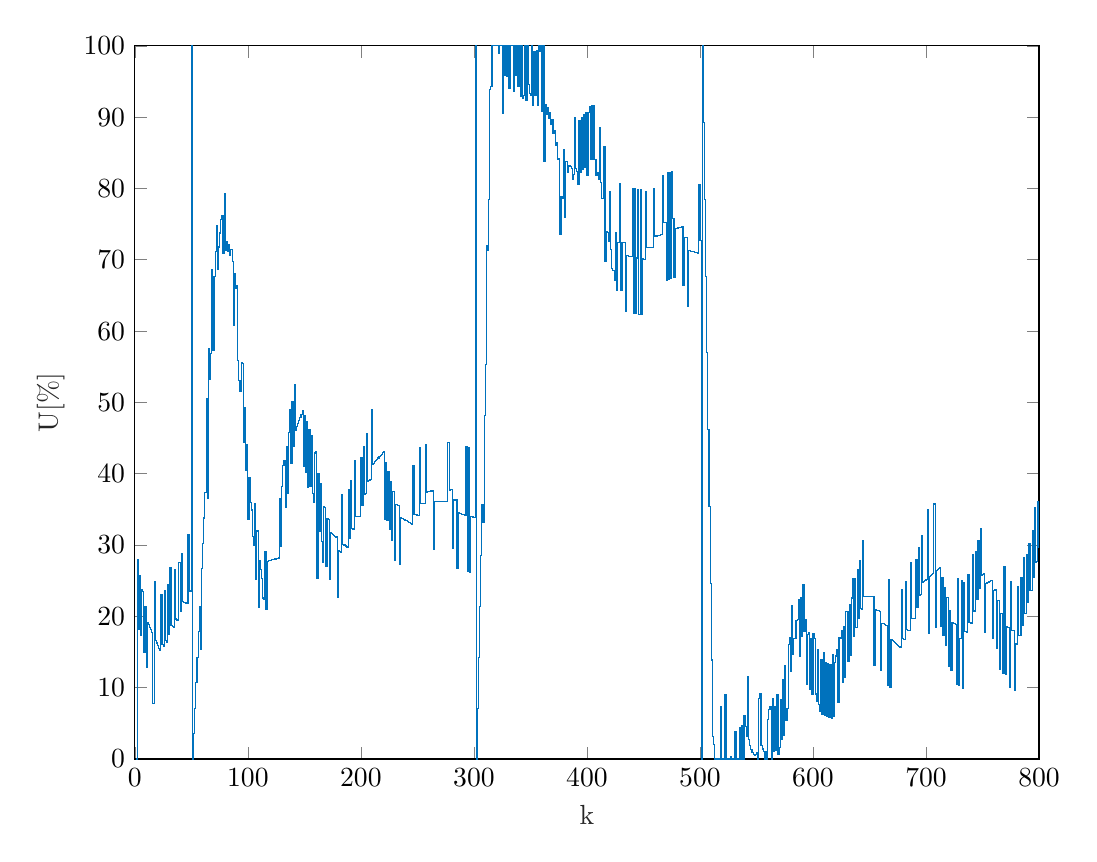
\begin{tikzpicture}

\begin{axis}[%
width=4.521in,
height=3.566in,
at={(0.758in,0.481in)},
scale only axis,
xmin=0,
xmax=800,
xlabel style={font=\color{white!15!black}},
xlabel={k},
ymin=0,
ymax=100,
ylabel style={font=\color{white!15!black}},
ylabel={U[\%]},
axis background/.style={fill=white}
]
\addplot[const plot, color=mycolor1, forget plot] table[row sep=crcr] {%
1	0\\
2	27.946429\\
3	18.117857\\
4	25.764286\\
5	17.264286\\
6	23.742857\\
7	23.471429\\
8	14.928571\\
9	21.364286\\
10	12.778571\\
11	19.171429\\
12	18.814286\\
13	18.457143\\
14	18.1\\
15	17.742857\\
16	7.735714\\
17	24.853571\\
18	16.621429\\
19	16.264286\\
20	15.907143\\
21	15.55\\
22	15.192857\\
23	23.107143\\
24	16.042857\\
25	15.728571\\
26	23.685714\\
27	16.664286\\
28	16.392857\\
29	24.392857\\
30	17.414286\\
31	26.835714\\
32	18.782143\\
33	18.603571\\
34	18.425\\
35	26.517857\\
36	19.632143\\
37	19.496429\\
38	19.360714\\
39	27.496429\\
40	20.653571\\
41	28.832143\\
42	22.032143\\
43	21.982143\\
44	21.932143\\
45	21.882143\\
46	21.832143\\
47	31.432143\\
48	23.557143\\
49	23.557143\\
50	100\\
51	0\\
52	3.571429\\
53	7.142857\\
54	10.714286\\
55	14.285714\\
56	17.857143\\
57	21.428571\\
58	15.35\\
59	26.746429\\
60	30.267857\\
61	33.789286\\
62	37.310714\\
63	50.482143\\
64	36.528571\\
65	57.575\\
66	53.271429\\
67	56.842857\\
68	68.685714\\
69	57.278571\\
70	67.6\\
71	71.171429\\
72	74.742857\\
73	68.664286\\
74	71.789286\\
75	73.746429\\
76	75.660714\\
77	76.153571\\
78	70.828571\\
79	79.314286\\
80	71.357143\\
81	72.560714\\
82	71.175\\
83	72.2\\
84	70.635714\\
85	71.482143\\
86	69.739286\\
87	60.757143\\
88	68.039286\\
89	65.982143\\
90	66.335714\\
91	55.828571\\
92	53.060714\\
93	51.535714\\
94	55.65\\
95	55.425\\
96	44.339286\\
97	49.264286\\
98	40.453571\\
99	44.032143\\
100	33.621429\\
101	39.475\\
102	35.989286\\
103	34.914286\\
104	31.25\\
105	29.996429\\
106	35.803571\\
107	25.167857\\
108	31.964286\\
109	21.192857\\
110	27.853571\\
111	26.596429\\
112	25.296429\\
113	22.575\\
114	22.307143\\
115	29.142857\\
116	20.957143\\
117	27.75\\
118	27.792857\\
119	27.835714\\
120	27.878571\\
121	27.921429\\
122	27.964286\\
123	28.007143\\
124	28.05\\
125	28.092857\\
126	28.135714\\
127	28.178571\\
128	36.492857\\
129	29.828571\\
130	38.185714\\
131	41.214286\\
132	41.789286\\
133	35.260714\\
134	43.753571\\
135	37.267857\\
136	45.803571\\
137	49.010714\\
138	41.492857\\
139	50.121429\\
140	43.771429\\
141	52.442857\\
142	46.135714\\
143	46.578571\\
144	47.021429\\
145	47.464286\\
146	47.907143\\
147	48.35\\
148	48.792857\\
149	40.964286\\
150	48.114286\\
151	40.242857\\
152	47.35\\
153	38.057143\\
154	46.239286\\
155	38.275\\
156	45.289286\\
157	37.282143\\
158	35.982143\\
159	42.910714\\
160	43.089286\\
161	25.346429\\
162	40.057143\\
163	31.871429\\
164	38.664286\\
165	30.435714\\
166	27.535714\\
167	35.360714\\
168	35.310714\\
169	26.989286\\
170	33.646429\\
171	33.553571\\
172	25.189286\\
173	31.803571\\
174	31.667857\\
175	31.532143\\
176	31.396429\\
177	31.260714\\
178	31.125\\
179	22.717857\\
180	29.289286\\
181	29.110714\\
182	28.932143\\
183	37.025\\
184	30.139286\\
185	30.003571\\
186	29.867857\\
187	29.732143\\
188	29.596429\\
189	37.732143\\
190	30.889286\\
191	39.067857\\
192	32.267857\\
193	32.217857\\
194	41.817857\\
195	33.942857\\
196	33.942857\\
197	33.942857\\
198	33.942857\\
199	33.942857\\
200	42.214286\\
201	35.507143\\
202	43.821429\\
203	37.157143\\
204	37.242857\\
205	45.6\\
206	38.978571\\
207	39.107143\\
208	39.235714\\
209	49.014286\\
210	41.317857\\
211	41.496429\\
212	41.675\\
213	41.853571\\
214	42.032143\\
215	42.210714\\
216	42.389286\\
217	42.567857\\
218	42.746429\\
219	42.925\\
220	43.103571\\
221	33.632143\\
222	41.635714\\
223	33.492857\\
224	40.328571\\
225	32.142857\\
226	38.935714\\
227	30.707143\\
228	37.457143\\
229	37.457143\\
230	27.807143\\
231	35.632143\\
232	35.582143\\
233	35.532143\\
234	27.210714\\
235	33.867857\\
236	33.775\\
237	33.682143\\
238	33.589286\\
239	33.496429\\
240	33.403571\\
241	33.310714\\
242	33.217857\\
243	33.125\\
244	33.032143\\
245	32.939286\\
246	41.117857\\
247	34.317857\\
248	34.267857\\
249	34.217857\\
250	34.167857\\
251	34.117857\\
252	43.717857\\
253	35.842857\\
254	35.842857\\
255	35.842857\\
256	35.842857\\
257	44.114286\\
258	37.407143\\
259	37.45\\
260	37.492857\\
261	37.535714\\
262	37.578571\\
263	37.621429\\
264	29.392857\\
265	36.142857\\
266	36.142857\\
267	36.142857\\
268	36.142857\\
269	36.142857\\
270	36.142857\\
271	36.142857\\
272	36.142857\\
273	36.142857\\
274	36.142857\\
275	36.142857\\
276	36.142857\\
277	44.414286\\
278	37.707143\\
279	37.75\\
280	37.792857\\
281	29.564286\\
282	36.314286\\
283	36.314286\\
284	36.314286\\
285	26.664286\\
286	34.489286\\
287	34.439286\\
288	34.389286\\
289	34.339286\\
290	34.289286\\
291	34.239286\\
292	34.189286\\
293	43.789286\\
294	26.264286\\
295	43.739286\\
296	26.214286\\
297	34.039286\\
298	33.989286\\
299	33.939286\\
300	33.889286\\
301	100\\
302	0\\
303	7.142857\\
304	14.285714\\
305	21.428571\\
306	28.571429\\
307	35.714286\\
308	33.207143\\
309	48.175\\
310	55.267857\\
311	72.010714\\
312	71.278571\\
313	78.421429\\
314	93.835714\\
315	94.271429\\
316	100\\
317	100\\
318	100\\
319	100\\
320	100\\
321	100\\
322	98.914286\\
323	100\\
324	100\\
325	90.55\\
326	100\\
327	95.792857\\
328	100\\
329	95.657143\\
330	100\\
331	93.957143\\
332	100\\
333	100\\
334	100\\
335	93.557143\\
336	100\\
337	95.832143\\
338	100\\
339	94.232143\\
340	100\\
341	92.885714\\
342	100\\
343	92.664286\\
344	93.067857\\
345	100\\
346	92.307143\\
347	100\\
348	94.582143\\
349	93.282143\\
350	92.971429\\
351	100\\
352	91.592857\\
353	99.196429\\
354	93.064286\\
355	99.321429\\
356	91.589286\\
357	100\\
358	99.192857\\
359	100\\
360	90.742857\\
361	100\\
362	83.814286\\
363	91.767857\\
364	90.382143\\
365	91.407143\\
366	89.842857\\
367	90.689286\\
368	88.946429\\
369	89.614286\\
370	87.692857\\
371	88.182143\\
372	86.082143\\
373	86.392857\\
374	84.114286\\
375	84.246429\\
376	73.517857\\
377	78.8\\
378	78.617857\\
379	85.496429\\
380	75.932143\\
381	83.8\\
382	83.75\\
383	82.278571\\
384	83.260714\\
385	83.075\\
386	82.846429\\
387	81.196429\\
388	82\\
389	89.907143\\
390	82.792857\\
391	82.385714\\
392	80.557143\\
393	89.453571\\
394	82.203571\\
395	89.932143\\
396	82.639286\\
397	90.325\\
398	82.989286\\
399	90.632143\\
400	81.875\\
401	90.592857\\
402	91.435714\\
403	84.007143\\
404	91.557143\\
405	84.085714\\
406	91.592857\\
407	84.078571\\
408	81.892857\\
409	82.160714\\
410	81.260714\\
411	88.589286\\
412	80.896429\\
413	78.532143\\
414	78.621429\\
415	85.814286\\
416	69.714286\\
417	73.921429\\
418	73.832143\\
419	72.575\\
420	79.546429\\
421	71.496429\\
422	68.775\\
423	68.507143\\
424	67.071429\\
425	73.864286\\
426	65.635714\\
427	72.385714\\
428	72.385714\\
429	80.657143\\
430	65.678571\\
431	72.428571\\
432	72.428571\\
433	72.428571\\
434	62.778571\\
435	70.603571\\
436	70.553571\\
437	70.503571\\
438	70.453571\\
439	70.403571\\
440	80.003571\\
441	62.478571\\
442	79.953571\\
443	62.428571\\
444	70.253571\\
445	79.853571\\
446	62.328571\\
447	79.803571\\
448	62.278571\\
449	70.103571\\
450	70.053571\\
451	70.003571\\
452	79.603571\\
453	71.728571\\
454	71.728571\\
455	71.728571\\
456	71.728571\\
457	71.728571\\
458	71.728571\\
459	80\\
460	73.292857\\
461	73.335714\\
462	73.378571\\
463	73.421429\\
464	73.464286\\
465	73.507143\\
466	73.55\\
467	81.864286\\
468	75.2\\
469	75.285714\\
470	67.1\\
471	82.164286\\
472	67.228571\\
473	82.292857\\
474	67.357143\\
475	82.421429\\
476	75.757143\\
477	67.571429\\
478	74.364286\\
479	74.407143\\
480	74.45\\
481	74.492857\\
482	74.535714\\
483	74.578571\\
484	74.621429\\
485	66.392857\\
486	73.142857\\
487	73.142857\\
488	73.142857\\
489	63.492857\\
490	71.317857\\
491	71.267857\\
492	71.217857\\
493	71.167857\\
494	71.117857\\
495	71.067857\\
496	71.017857\\
497	70.967857\\
498	70.917857\\
499	80.517857\\
500	72.642857\\
501	0\\
502	100\\
503	89.235714\\
504	78.471429\\
505	67.707143\\
506	56.942857\\
507	46.178571\\
508	35.414286\\
509	24.65\\
510	13.885714\\
511	3.121429\\
512	2.007143\\
513	0\\
514	0\\
515	0\\
516	0\\
517	0\\
518	7.292857\\
519	0\\
520	0\\
521	0\\
522	9.035714\\
523	0\\
524	0.010714\\
525	0\\
526	0\\
527	0.367857\\
528	0\\
529	0\\
530	0\\
531	3.803571\\
532	0\\
533	0\\
534	0\\
535	4.382143\\
536	0\\
537	4.696429\\
538	0\\
539	6.128571\\
540	4.560714\\
541	3.171429\\
542	11.610714\\
543	2.753571\\
544	1.95\\
545	1.325\\
546	0.878571\\
547	0.610714\\
548	0.521429\\
549	0.610714\\
550	0.878571\\
551	0\\
552	8.45\\
553	9.203571\\
554	1.864286\\
555	1.410714\\
556	1.092857\\
557	0\\
558	1.071429\\
559	0\\
560	5.546429\\
561	6.975\\
562	7.414286\\
563	0\\
564	8.535714\\
565	1.060714\\
566	7.321429\\
567	1.192857\\
568	9.053571\\
569	0.65\\
570	1.585714\\
571	8.382143\\
572	2.789286\\
573	11.185714\\
574	3.317857\\
575	13.060714\\
576	5.414286\\
577	7.107143\\
578	16.039286\\
579	16.978571\\
580	12.278571\\
581	21.567857\\
582	14.592857\\
583	16.957143\\
584	16.910714\\
585	19.453571\\
586	19.585714\\
587	22.307143\\
588	14.346429\\
589	22.575\\
590	17.246429\\
591	24.485714\\
592	17.914286\\
593	19.514286\\
594	10.389286\\
595	17.410714\\
596	17.725\\
597	9.810714\\
598	16.917857\\
599	9.046429\\
600	17.575\\
601	16.9\\
602	9.121429\\
603	8.092857\\
604	15.335714\\
605	7.6\\
606	6.614286\\
607	13.9\\
608	6.207143\\
609	14.914286\\
610	6.146429\\
611	13.525\\
612	5.925\\
613	13.346429\\
614	5.789286\\
615	13.253571\\
616	5.739286\\
617	14.625\\
618	6.035714\\
619	13.592857\\
620	14.442857\\
621	15.335714\\
622	8\\
623	17.064286\\
624	16.925\\
625	17.953571\\
626	10.753571\\
627	18.575\\
628	11.417857\\
629	20.660714\\
630	20.7\\
631	13.635714\\
632	21.592857\\
633	14.571429\\
634	22.571429\\
635	25.242857\\
636	17.189286\\
637	25.282143\\
638	18.396429\\
639	26.532143\\
640	19.689286\\
641	27.867857\\
642	21.067857\\
643	21.017857\\
644	30.617857\\
645	22.742857\\
646	22.742857\\
647	22.742857\\
648	22.742857\\
649	22.742857\\
650	22.742857\\
651	22.742857\\
652	22.742857\\
653	22.742857\\
654	13.092857\\
655	20.917857\\
656	20.867857\\
657	20.817857\\
658	20.767857\\
659	20.717857\\
660	12.396429\\
661	19.053571\\
662	18.960714\\
663	18.867857\\
664	18.775\\
665	18.682143\\
666	10.317857\\
667	25.203571\\
668	10.089286\\
669	16.703571\\
670	16.567857\\
671	16.432143\\
672	16.296429\\
673	16.160714\\
674	16.025\\
675	15.889286\\
676	15.753571\\
677	15.617857\\
678	23.753571\\
679	16.910714\\
680	16.817857\\
681	16.725\\
682	24.903571\\
683	18.103571\\
684	18.053571\\
685	18.003571\\
686	27.603571\\
687	19.728571\\
688	19.728571\\
689	19.728571\\
690	19.728571\\
691	28\\
692	21.292857\\
693	29.607143\\
694	22.942857\\
695	23.028571\\
696	31.385714\\
697	24.764286\\
698	24.892857\\
699	25.021429\\
700	25.15\\
701	34.928571\\
702	17.582143\\
703	25.585714\\
704	25.714286\\
705	25.842857\\
706	25.971429\\
707	35.75\\
708	18.403571\\
709	26.407143\\
710	26.535714\\
711	26.664286\\
712	26.792857\\
713	18.65\\
714	25.485714\\
715	17.3\\
716	24.092857\\
717	15.864286\\
718	22.614286\\
719	22.614286\\
720	12.964286\\
721	20.789286\\
722	12.467857\\
723	19.125\\
724	19.032143\\
725	18.939286\\
726	18.846429\\
727	10.482143\\
728	25.367857\\
729	10.253571\\
730	16.867857\\
731	25.003571\\
732	9.889286\\
733	24.775\\
734	17.932143\\
735	17.839286\\
736	17.746429\\
737	25.925\\
738	19.125\\
739	19.075\\
740	19.025\\
741	28.625\\
742	20.75\\
743	20.75\\
744	29.021429\\
745	22.314286\\
746	30.628571\\
747	23.964286\\
748	32.321429\\
749	25.7\\
750	25.828571\\
751	25.957143\\
752	17.814286\\
753	24.65\\
754	24.735714\\
755	24.821429\\
756	24.907143\\
757	24.992857\\
758	25.078571\\
759	16.892857\\
760	23.685714\\
761	23.728571\\
762	15.5\\
763	22.25\\
764	22.25\\
765	12.6\\
766	20.425\\
767	20.375\\
768	12.053571\\
769	26.982143\\
770	11.910714\\
771	18.567857\\
772	18.475\\
773	18.382143\\
774	10.017857\\
775	24.903571\\
776	18.060714\\
777	17.967857\\
778	9.603571\\
779	16.217857\\
780	16.082143\\
781	24.217857\\
782	17.375\\
783	17.282143\\
784	25.460714\\
785	18.660714\\
786	28.260714\\
787	20.385714\\
788	20.385714\\
789	28.657143\\
790	21.95\\
791	30.264286\\
792	23.6\\
793	23.685714\\
794	32.042857\\
795	25.421429\\
796	35.2\\
797	27.503571\\
798	27.682143\\
799	36.132143\\
800	29.603571\\
};
\end{axis}
\end{tikzpicture}%
\caption{Sterowanie PID z laboratorium 1}
\end{figure}

Wartość wskaźnika jakości:

\begin{equation}
E = 19,3149e+07
\end{equation}

\subsection{DMC z laboratorium 1}

Wykorzystaliśmy parametry DMC z laboratorium drugiego:

\begin{equation}
N = 90; 
N_u = 10; 
\lambda = 0,4; 
\end{equation}
 
Wyniki działania regulacji:

\begin{figure}[H]
\centering
% This file was created by matlab2tikz.
%
%The latest updates can be retrieved from
%  http://www.mathworks.com/matlabcentral/fileexchange/22022-matlab2tikz-matlab2tikz
%where you can also make suggestions and rate matlab2tikz.
%
\definecolor{mycolor1}{rgb}{0.00000,0.44700,0.74100}%
\definecolor{mycolor2}{rgb}{0.85000,0.32500,0.09800}%
%
\begin{tikzpicture}

\begin{axis}[%
width=4.521in,
height=3.566in,
at={(0.758in,0.481in)},
scale only axis,
xmin=0,
xmax=800,
xlabel style={font=\color{white!15!black}},
xlabel={k},
ymin=30,
ymax=48,
ylabel style={font=\color{white!15!black}},
ylabel={$\text{T[}^\circ\text{C]}$},
axis background/.style={fill=white},
legend style={legend cell align=left, align=left, draw=white!15!black}
]
\addplot[const plot, color=mycolor1] table[row sep=crcr] {%
1	31.87\\
2	31.81\\
3	31.75\\
4	31.68\\
5	31.62\\
6	31.56\\
7	31.56\\
8	31.56\\
9	31.5\\
10	31.5\\
11	31.5\\
12	31.43\\
13	31.43\\
14	31.37\\
15	31.37\\
16	31.37\\
17	31.37\\
18	31.37\\
19	31.31\\
20	31.31\\
21	31.31\\
22	31.31\\
23	31.31\\
24	31.31\\
25	31.31\\
26	31.31\\
27	31.25\\
28	31.25\\
29	31.25\\
30	31.18\\
31	31.18\\
32	31.18\\
33	31.12\\
34	31.12\\
35	31.12\\
36	31.12\\
37	31.12\\
38	31.12\\
39	31.12\\
40	31.12\\
41	31.12\\
42	31.12\\
43	31.12\\
44	31.12\\
45	31.12\\
46	31.12\\
47	31.12\\
48	31.12\\
49	31.12\\
50	31.12\\
51	31.12\\
52	31.18\\
53	31.18\\
54	31.18\\
55	31.18\\
56	31.18\\
57	31.18\\
58	31.18\\
59	31.25\\
60	31.25\\
61	31.31\\
62	31.37\\
63	31.37\\
64	31.43\\
65	31.5\\
66	31.56\\
67	31.62\\
68	31.75\\
69	31.75\\
70	31.93\\
71	32\\
72	32.12\\
73	32.25\\
74	32.37\\
75	32.5\\
76	32.68\\
77	32.81\\
78	32.93\\
79	33.06\\
80	33.18\\
81	33.31\\
82	33.43\\
83	33.56\\
84	33.75\\
85	33.87\\
86	33.93\\
87	34.06\\
88	34.18\\
89	34.31\\
90	34.43\\
91	34.5\\
92	34.56\\
93	34.68\\
94	34.75\\
95	34.81\\
96	34.87\\
97	35\\
98	35.06\\
99	35.06\\
100	35.12\\
101	35.18\\
102	35.25\\
103	35.25\\
104	35.31\\
105	35.37\\
106	35.37\\
107	35.43\\
108	35.43\\
109	35.43\\
110	35.43\\
111	35.43\\
112	35.5\\
113	35.5\\
114	35.5\\
115	35.5\\
116	35.5\\
117	35.5\\
118	35.5\\
119	35.5\\
120	35.56\\
121	35.56\\
122	35.56\\
123	35.56\\
124	35.56\\
125	35.56\\
126	35.56\\
127	35.56\\
128	35.56\\
129	35.56\\
130	35.56\\
131	35.56\\
132	35.5\\
133	35.5\\
134	35.5\\
135	35.5\\
136	35.5\\
137	35.5\\
138	35.5\\
139	35.5\\
140	35.5\\
141	35.5\\
142	35.5\\
143	35.5\\
144	35.5\\
145	35.5\\
146	35.5\\
147	35.5\\
148	35.5\\
149	35.5\\
150	35.5\\
151	35.43\\
152	35.43\\
153	35.43\\
154	35.43\\
155	35.43\\
156	35.43\\
157	35.43\\
158	35.43\\
159	35.5\\
160	35.5\\
161	35.5\\
162	35.5\\
163	35.5\\
164	35.5\\
165	35.5\\
166	35.5\\
167	35.5\\
168	35.56\\
169	35.56\\
170	35.5\\
171	35.56\\
172	35.56\\
173	35.56\\
174	35.62\\
175	35.62\\
176	35.62\\
177	35.56\\
178	35.62\\
179	35.56\\
180	35.62\\
181	35.62\\
182	35.62\\
183	35.68\\
184	35.68\\
185	35.68\\
186	35.68\\
187	35.68\\
188	35.68\\
189	35.68\\
190	35.75\\
191	35.68\\
192	35.75\\
193	35.75\\
194	35.68\\
195	35.75\\
196	35.68\\
197	35.75\\
198	35.75\\
199	35.75\\
200	35.81\\
201	35.81\\
202	35.81\\
203	35.81\\
204	35.81\\
205	35.81\\
206	35.81\\
207	35.75\\
208	35.75\\
209	35.75\\
210	35.75\\
211	35.75\\
212	35.75\\
213	35.75\\
214	35.75\\
215	35.75\\
216	35.75\\
217	35.75\\
218	35.81\\
219	35.81\\
220	35.81\\
221	35.81\\
222	35.75\\
223	35.75\\
224	35.75\\
225	35.75\\
226	35.75\\
227	35.68\\
228	35.75\\
229	35.68\\
230	35.75\\
231	35.75\\
232	35.75\\
233	35.75\\
234	35.75\\
235	35.75\\
236	35.68\\
237	35.75\\
238	35.75\\
239	35.75\\
240	35.75\\
241	35.75\\
242	35.75\\
243	35.81\\
244	35.81\\
245	35.81\\
246	35.81\\
247	35.87\\
248	35.87\\
249	35.87\\
250	35.87\\
251	35.87\\
252	35.87\\
253	35.87\\
254	35.87\\
255	35.87\\
256	35.87\\
257	35.87\\
258	35.87\\
259	35.81\\
260	35.81\\
261	35.81\\
262	35.81\\
263	35.81\\
264	35.81\\
265	35.81\\
266	35.81\\
267	35.81\\
268	35.81\\
269	35.81\\
270	35.81\\
271	35.81\\
272	35.81\\
273	35.81\\
274	35.81\\
275	35.81\\
276	35.81\\
277	35.87\\
278	35.87\\
279	35.81\\
280	35.81\\
281	35.81\\
282	35.81\\
283	35.81\\
284	35.81\\
285	35.81\\
286	35.81\\
287	35.81\\
288	35.81\\
289	35.81\\
290	35.81\\
291	35.81\\
292	35.87\\
293	35.87\\
294	35.87\\
295	35.87\\
296	35.87\\
297	35.87\\
298	35.87\\
299	35.87\\
300	35.93\\
301	35.93\\
302	35.93\\
303	35.93\\
304	35.93\\
305	35.93\\
306	36\\
307	36\\
308	36\\
309	36\\
310	36\\
311	36.06\\
312	36.06\\
313	36.12\\
314	36.18\\
315	36.25\\
316	36.31\\
317	36.43\\
318	36.5\\
319	36.62\\
320	36.75\\
321	36.81\\
322	37\\
323	37.12\\
324	37.25\\
325	37.37\\
326	37.56\\
327	37.68\\
328	37.87\\
329	38\\
330	38.18\\
331	38.31\\
332	38.5\\
333	38.62\\
334	38.81\\
335	38.93\\
336	39.12\\
337	39.25\\
338	39.37\\
339	39.5\\
340	39.62\\
341	39.75\\
342	39.87\\
343	40\\
344	40.18\\
345	40.31\\
346	40.43\\
347	40.56\\
348	40.68\\
349	40.81\\
350	40.87\\
351	40.93\\
352	41.06\\
353	41.12\\
354	41.18\\
355	41.25\\
356	41.31\\
357	41.37\\
358	41.37\\
359	41.43\\
360	41.5\\
361	41.56\\
362	41.56\\
363	41.62\\
364	41.68\\
365	41.75\\
366	41.81\\
367	41.81\\
368	41.87\\
369	41.87\\
370	41.93\\
371	41.93\\
372	41.93\\
373	42\\
374	42.06\\
375	42.06\\
376	42.06\\
377	42.12\\
378	42.18\\
379	42.18\\
380	42.31\\
381	42.37\\
382	42.37\\
383	42.43\\
384	42.5\\
385	42.5\\
386	42.56\\
387	42.56\\
388	42.62\\
389	42.62\\
390	42.62\\
391	42.68\\
392	42.68\\
393	42.68\\
394	42.68\\
395	42.68\\
396	42.75\\
397	42.75\\
398	42.81\\
399	42.81\\
400	42.87\\
401	42.87\\
402	42.93\\
403	42.93\\
404	43\\
405	43\\
406	43.06\\
407	43.06\\
408	43.06\\
409	43.06\\
410	43.12\\
411	43.12\\
412	43.12\\
413	43.12\\
414	43.12\\
415	43.18\\
416	43.25\\
417	43.25\\
418	43.25\\
419	43.31\\
420	43.31\\
421	43.31\\
422	43.37\\
423	43.37\\
424	43.43\\
425	43.5\\
426	43.5\\
427	43.43\\
428	43.43\\
429	43.5\\
430	43.43\\
431	43.43\\
432	43.5\\
433	43.5\\
434	43.5\\
435	43.56\\
436	43.56\\
437	43.56\\
438	43.62\\
439	43.62\\
440	43.62\\
441	43.68\\
442	43.68\\
443	43.68\\
444	43.75\\
445	43.75\\
446	43.75\\
447	43.75\\
448	43.75\\
449	43.75\\
450	43.75\\
451	43.81\\
452	43.87\\
453	43.93\\
454	43.93\\
455	44\\
456	44\\
457	44\\
458	44\\
459	44.06\\
460	44.06\\
461	44.06\\
462	44.12\\
463	44.12\\
464	44.06\\
465	44.12\\
466	44.06\\
467	44.06\\
468	44.06\\
469	44.06\\
470	44.06\\
471	44\\
472	44.06\\
473	44.06\\
474	44.06\\
475	44.12\\
476	44.12\\
477	44.12\\
478	44.18\\
479	44.25\\
480	44.25\\
481	44.31\\
482	44.31\\
483	44.31\\
484	44.31\\
485	44.31\\
486	44.37\\
487	44.37\\
488	44.43\\
489	44.43\\
490	44.43\\
491	44.43\\
492	44.5\\
493	44.5\\
494	44.43\\
495	44.5\\
496	44.5\\
497	44.56\\
498	44.62\\
499	44.62\\
500	44.68\\
501	44.68\\
502	44.75\\
503	44.75\\
504	44.75\\
505	44.81\\
506	44.81\\
507	44.81\\
508	44.81\\
509	44.81\\
510	44.75\\
511	44.75\\
512	44.68\\
513	44.56\\
514	44.5\\
515	44.43\\
516	44.31\\
517	44.18\\
518	44.06\\
519	43.93\\
520	43.75\\
521	43.56\\
522	43.37\\
523	43.12\\
524	42.93\\
525	42.75\\
526	42.56\\
527	42.31\\
528	42.12\\
529	41.87\\
530	41.68\\
531	41.5\\
532	41.25\\
533	41.06\\
534	40.87\\
535	40.68\\
536	40.56\\
537	40.37\\
538	40.25\\
539	40.06\\
540	39.93\\
541	39.81\\
542	39.68\\
543	39.56\\
544	39.43\\
545	39.37\\
546	39.31\\
547	39.25\\
548	39.18\\
549	39.12\\
550	39.06\\
551	39.06\\
552	39.06\\
553	39.06\\
554	39.06\\
555	39.06\\
556	39.06\\
557	39.06\\
558	39.06\\
559	39.12\\
560	39.12\\
561	39.12\\
562	39.18\\
563	39.18\\
564	39.25\\
565	39.25\\
566	39.25\\
567	39.25\\
568	39.31\\
569	39.31\\
570	39.31\\
571	39.31\\
572	39.31\\
573	39.31\\
574	39.31\\
575	39.31\\
576	39.31\\
577	39.25\\
578	39.31\\
579	39.25\\
580	39.25\\
581	39.25\\
582	39.18\\
583	39.18\\
584	39.12\\
585	39.12\\
586	39.06\\
587	39.06\\
588	39.06\\
589	39\\
590	39\\
591	38.93\\
592	38.87\\
593	38.81\\
594	38.81\\
595	38.75\\
596	38.75\\
597	38.75\\
598	38.68\\
599	38.68\\
600	38.68\\
601	38.62\\
602	38.62\\
603	38.56\\
604	38.5\\
605	38.43\\
606	38.37\\
607	38.37\\
608	38.31\\
609	38.25\\
610	38.25\\
611	38.18\\
612	38.12\\
613	38.06\\
614	38\\
615	37.93\\
616	37.87\\
617	37.81\\
618	37.81\\
619	37.75\\
620	37.68\\
621	37.62\\
622	37.62\\
623	37.56\\
624	37.5\\
625	37.5\\
626	37.43\\
627	37.43\\
628	37.37\\
629	37.31\\
630	37.31\\
631	37.25\\
632	37.18\\
633	37.12\\
634	37\\
635	37\\
636	36.93\\
637	36.87\\
638	36.81\\
639	36.75\\
640	36.68\\
641	36.68\\
642	36.62\\
643	36.56\\
644	36.5\\
645	36.5\\
646	36.37\\
647	36.37\\
648	36.31\\
649	36.25\\
650	36.25\\
651	36.18\\
652	36.12\\
653	36.06\\
654	36.06\\
655	36\\
656	36\\
657	35.93\\
658	35.87\\
659	35.81\\
660	35.75\\
661	35.68\\
662	35.68\\
663	35.62\\
664	35.56\\
665	35.56\\
666	35.5\\
667	35.5\\
668	35.43\\
669	35.37\\
670	35.37\\
671	35.31\\
672	35.31\\
673	35.25\\
674	35.18\\
675	35.12\\
676	35.06\\
677	35.06\\
678	35\\
679	34.93\\
680	34.93\\
681	34.87\\
682	34.87\\
683	34.81\\
684	34.75\\
685	34.75\\
686	34.68\\
687	34.68\\
688	34.62\\
689	34.56\\
690	34.56\\
691	34.56\\
692	34.5\\
693	34.5\\
694	34.5\\
695	34.43\\
696	34.43\\
697	34.37\\
698	34.37\\
699	34.31\\
700	34.31\\
701	34.31\\
702	34.25\\
703	34.25\\
704	34.25\\
705	34.25\\
706	34.25\\
707	34.25\\
708	34.25\\
709	34.25\\
710	34.25\\
711	34.25\\
712	34.18\\
713	34.18\\
714	34.18\\
715	34.18\\
716	34.12\\
717	34.12\\
718	34.12\\
719	34.12\\
720	34.06\\
721	34.06\\
722	34.06\\
723	34\\
724	34\\
725	33.93\\
726	33.87\\
727	33.87\\
728	33.87\\
729	33.81\\
730	33.81\\
731	33.75\\
732	33.68\\
733	33.68\\
734	33.68\\
735	33.62\\
736	33.62\\
737	33.62\\
738	33.56\\
739	33.56\\
740	33.5\\
741	33.5\\
742	33.43\\
743	33.43\\
744	33.43\\
745	33.37\\
746	33.37\\
747	33.37\\
748	33.31\\
749	33.31\\
750	33.31\\
751	33.31\\
752	33.25\\
753	33.25\\
754	33.25\\
755	33.25\\
756	33.18\\
757	33.12\\
758	33.12\\
759	33.06\\
760	33.06\\
761	33\\
762	33\\
763	33\\
764	32.93\\
765	32.93\\
766	32.87\\
767	32.87\\
768	32.81\\
769	32.81\\
770	32.75\\
771	32.75\\
772	32.75\\
773	32.75\\
774	32.68\\
775	32.62\\
776	32.62\\
777	32.62\\
778	32.56\\
779	32.56\\
780	32.56\\
781	32.56\\
782	32.5\\
783	32.5\\
784	32.5\\
785	32.43\\
786	32.43\\
787	32.37\\
788	32.37\\
789	32.37\\
790	32.37\\
791	32.31\\
792	32.31\\
793	32.25\\
794	32.25\\
795	32.18\\
796	32.18\\
797	32.18\\
798	32.12\\
799	32.12\\
800	32.06\\
};
\addlegendentry{Y}

\addplot[const plot, color=mycolor2, dashed] table[row sep=crcr] {%
1	30.93\\
2	30.93\\
3	30.93\\
4	30.93\\
5	30.93\\
6	30.93\\
7	30.93\\
8	30.93\\
9	30.93\\
10	30.93\\
11	30.93\\
12	30.93\\
13	30.93\\
14	30.93\\
15	30.93\\
16	30.93\\
17	30.93\\
18	30.93\\
19	30.93\\
20	30.93\\
21	30.93\\
22	30.93\\
23	30.93\\
24	30.93\\
25	30.93\\
26	30.93\\
27	30.93\\
28	30.93\\
29	30.93\\
30	30.93\\
31	30.93\\
32	30.93\\
33	30.93\\
34	30.93\\
35	30.93\\
36	30.93\\
37	30.93\\
38	30.93\\
39	30.93\\
40	30.93\\
41	30.93\\
42	30.93\\
43	30.93\\
44	30.93\\
45	30.93\\
46	30.93\\
47	30.93\\
48	30.93\\
49	30.93\\
50	30.93\\
51	35.93\\
52	35.93\\
53	35.93\\
54	35.93\\
55	35.93\\
56	35.93\\
57	35.93\\
58	35.93\\
59	35.93\\
60	35.93\\
61	35.93\\
62	35.93\\
63	35.93\\
64	35.93\\
65	35.93\\
66	35.93\\
67	35.93\\
68	35.93\\
69	35.93\\
70	35.93\\
71	35.93\\
72	35.93\\
73	35.93\\
74	35.93\\
75	35.93\\
76	35.93\\
77	35.93\\
78	35.93\\
79	35.93\\
80	35.93\\
81	35.93\\
82	35.93\\
83	35.93\\
84	35.93\\
85	35.93\\
86	35.93\\
87	35.93\\
88	35.93\\
89	35.93\\
90	35.93\\
91	35.93\\
92	35.93\\
93	35.93\\
94	35.93\\
95	35.93\\
96	35.93\\
97	35.93\\
98	35.93\\
99	35.93\\
100	35.93\\
101	35.93\\
102	35.93\\
103	35.93\\
104	35.93\\
105	35.93\\
106	35.93\\
107	35.93\\
108	35.93\\
109	35.93\\
110	35.93\\
111	35.93\\
112	35.93\\
113	35.93\\
114	35.93\\
115	35.93\\
116	35.93\\
117	35.93\\
118	35.93\\
119	35.93\\
120	35.93\\
121	35.93\\
122	35.93\\
123	35.93\\
124	35.93\\
125	35.93\\
126	35.93\\
127	35.93\\
128	35.93\\
129	35.93\\
130	35.93\\
131	35.93\\
132	35.93\\
133	35.93\\
134	35.93\\
135	35.93\\
136	35.93\\
137	35.93\\
138	35.93\\
139	35.93\\
140	35.93\\
141	35.93\\
142	35.93\\
143	35.93\\
144	35.93\\
145	35.93\\
146	35.93\\
147	35.93\\
148	35.93\\
149	35.93\\
150	35.93\\
151	35.93\\
152	35.93\\
153	35.93\\
154	35.93\\
155	35.93\\
156	35.93\\
157	35.93\\
158	35.93\\
159	35.93\\
160	35.93\\
161	35.93\\
162	35.93\\
163	35.93\\
164	35.93\\
165	35.93\\
166	35.93\\
167	35.93\\
168	35.93\\
169	35.93\\
170	35.93\\
171	35.93\\
172	35.93\\
173	35.93\\
174	35.93\\
175	35.93\\
176	35.93\\
177	35.93\\
178	35.93\\
179	35.93\\
180	35.93\\
181	35.93\\
182	35.93\\
183	35.93\\
184	35.93\\
185	35.93\\
186	35.93\\
187	35.93\\
188	35.93\\
189	35.93\\
190	35.93\\
191	35.93\\
192	35.93\\
193	35.93\\
194	35.93\\
195	35.93\\
196	35.93\\
197	35.93\\
198	35.93\\
199	35.93\\
200	35.93\\
201	35.93\\
202	35.93\\
203	35.93\\
204	35.93\\
205	35.93\\
206	35.93\\
207	35.93\\
208	35.93\\
209	35.93\\
210	35.93\\
211	35.93\\
212	35.93\\
213	35.93\\
214	35.93\\
215	35.93\\
216	35.93\\
217	35.93\\
218	35.93\\
219	35.93\\
220	35.93\\
221	35.93\\
222	35.93\\
223	35.93\\
224	35.93\\
225	35.93\\
226	35.93\\
227	35.93\\
228	35.93\\
229	35.93\\
230	35.93\\
231	35.93\\
232	35.93\\
233	35.93\\
234	35.93\\
235	35.93\\
236	35.93\\
237	35.93\\
238	35.93\\
239	35.93\\
240	35.93\\
241	35.93\\
242	35.93\\
243	35.93\\
244	35.93\\
245	35.93\\
246	35.93\\
247	35.93\\
248	35.93\\
249	35.93\\
250	35.93\\
251	35.93\\
252	35.93\\
253	35.93\\
254	35.93\\
255	35.93\\
256	35.93\\
257	35.93\\
258	35.93\\
259	35.93\\
260	35.93\\
261	35.93\\
262	35.93\\
263	35.93\\
264	35.93\\
265	35.93\\
266	35.93\\
267	35.93\\
268	35.93\\
269	35.93\\
270	35.93\\
271	35.93\\
272	35.93\\
273	35.93\\
274	35.93\\
275	35.93\\
276	35.93\\
277	35.93\\
278	35.93\\
279	35.93\\
280	35.93\\
281	35.93\\
282	35.93\\
283	35.93\\
284	35.93\\
285	35.93\\
286	35.93\\
287	35.93\\
288	35.93\\
289	35.93\\
290	35.93\\
291	35.93\\
292	35.93\\
293	35.93\\
294	35.93\\
295	35.93\\
296	35.93\\
297	35.93\\
298	35.93\\
299	35.93\\
300	35.93\\
301	45.93\\
302	45.93\\
303	45.93\\
304	45.93\\
305	45.93\\
306	45.93\\
307	45.93\\
308	45.93\\
309	45.93\\
310	45.93\\
311	45.93\\
312	45.93\\
313	45.93\\
314	45.93\\
315	45.93\\
316	45.93\\
317	45.93\\
318	45.93\\
319	45.93\\
320	45.93\\
321	45.93\\
322	45.93\\
323	45.93\\
324	45.93\\
325	45.93\\
326	45.93\\
327	45.93\\
328	45.93\\
329	45.93\\
330	45.93\\
331	45.93\\
332	45.93\\
333	45.93\\
334	45.93\\
335	45.93\\
336	45.93\\
337	45.93\\
338	45.93\\
339	45.93\\
340	45.93\\
341	45.93\\
342	45.93\\
343	45.93\\
344	45.93\\
345	45.93\\
346	45.93\\
347	45.93\\
348	45.93\\
349	45.93\\
350	45.93\\
351	45.93\\
352	45.93\\
353	45.93\\
354	45.93\\
355	45.93\\
356	45.93\\
357	45.93\\
358	45.93\\
359	45.93\\
360	45.93\\
361	45.93\\
362	45.93\\
363	45.93\\
364	45.93\\
365	45.93\\
366	45.93\\
367	45.93\\
368	45.93\\
369	45.93\\
370	45.93\\
371	45.93\\
372	45.93\\
373	45.93\\
374	45.93\\
375	45.93\\
376	45.93\\
377	45.93\\
378	45.93\\
379	45.93\\
380	45.93\\
381	45.93\\
382	45.93\\
383	45.93\\
384	45.93\\
385	45.93\\
386	45.93\\
387	45.93\\
388	45.93\\
389	45.93\\
390	45.93\\
391	45.93\\
392	45.93\\
393	45.93\\
394	45.93\\
395	45.93\\
396	45.93\\
397	45.93\\
398	45.93\\
399	45.93\\
400	45.93\\
401	45.93\\
402	45.93\\
403	45.93\\
404	45.93\\
405	45.93\\
406	45.93\\
407	45.93\\
408	45.93\\
409	45.93\\
410	45.93\\
411	45.93\\
412	45.93\\
413	45.93\\
414	45.93\\
415	45.93\\
416	45.93\\
417	45.93\\
418	45.93\\
419	45.93\\
420	45.93\\
421	45.93\\
422	45.93\\
423	45.93\\
424	45.93\\
425	45.93\\
426	45.93\\
427	45.93\\
428	45.93\\
429	45.93\\
430	45.93\\
431	45.93\\
432	45.93\\
433	45.93\\
434	45.93\\
435	45.93\\
436	45.93\\
437	45.93\\
438	45.93\\
439	45.93\\
440	45.93\\
441	45.93\\
442	45.93\\
443	45.93\\
444	45.93\\
445	45.93\\
446	45.93\\
447	45.93\\
448	45.93\\
449	45.93\\
450	45.93\\
451	45.93\\
452	45.93\\
453	45.93\\
454	45.93\\
455	45.93\\
456	45.93\\
457	45.93\\
458	45.93\\
459	45.93\\
460	45.93\\
461	45.93\\
462	45.93\\
463	45.93\\
464	45.93\\
465	45.93\\
466	45.93\\
467	45.93\\
468	45.93\\
469	45.93\\
470	45.93\\
471	45.93\\
472	45.93\\
473	45.93\\
474	45.93\\
475	45.93\\
476	45.93\\
477	45.93\\
478	45.93\\
479	45.93\\
480	45.93\\
481	45.93\\
482	45.93\\
483	45.93\\
484	45.93\\
485	45.93\\
486	45.93\\
487	45.93\\
488	45.93\\
489	45.93\\
490	45.93\\
491	45.93\\
492	45.93\\
493	45.93\\
494	45.93\\
495	45.93\\
496	45.93\\
497	45.93\\
498	45.93\\
499	45.93\\
500	45.93\\
501	30.93\\
502	30.93\\
503	30.93\\
504	30.93\\
505	30.93\\
506	30.93\\
507	30.93\\
508	30.93\\
509	30.93\\
510	30.93\\
511	30.93\\
512	30.93\\
513	30.93\\
514	30.93\\
515	30.93\\
516	30.93\\
517	30.93\\
518	30.93\\
519	30.93\\
520	30.93\\
521	30.93\\
522	30.93\\
523	30.93\\
524	30.93\\
525	30.93\\
526	30.93\\
527	30.93\\
528	30.93\\
529	30.93\\
530	30.93\\
531	30.93\\
532	30.93\\
533	30.93\\
534	30.93\\
535	30.93\\
536	30.93\\
537	30.93\\
538	30.93\\
539	30.93\\
540	30.93\\
541	30.93\\
542	30.93\\
543	30.93\\
544	30.93\\
545	30.93\\
546	30.93\\
547	30.93\\
548	30.93\\
549	30.93\\
550	30.93\\
551	30.93\\
552	30.93\\
553	30.93\\
554	30.93\\
555	30.93\\
556	30.93\\
557	30.93\\
558	30.93\\
559	30.93\\
560	30.93\\
561	30.93\\
562	30.93\\
563	30.93\\
564	30.93\\
565	30.93\\
566	30.93\\
567	30.93\\
568	30.93\\
569	30.93\\
570	30.93\\
571	30.93\\
572	30.93\\
573	30.93\\
574	30.93\\
575	30.93\\
576	30.93\\
577	30.93\\
578	30.93\\
579	30.93\\
580	30.93\\
581	30.93\\
582	30.93\\
583	30.93\\
584	30.93\\
585	30.93\\
586	30.93\\
587	30.93\\
588	30.93\\
589	30.93\\
590	30.93\\
591	30.93\\
592	30.93\\
593	30.93\\
594	30.93\\
595	30.93\\
596	30.93\\
597	30.93\\
598	30.93\\
599	30.93\\
600	30.93\\
601	30.93\\
602	30.93\\
603	30.93\\
604	30.93\\
605	30.93\\
606	30.93\\
607	30.93\\
608	30.93\\
609	30.93\\
610	30.93\\
611	30.93\\
612	30.93\\
613	30.93\\
614	30.93\\
615	30.93\\
616	30.93\\
617	30.93\\
618	30.93\\
619	30.93\\
620	30.93\\
621	30.93\\
622	30.93\\
623	30.93\\
624	30.93\\
625	30.93\\
626	30.93\\
627	30.93\\
628	30.93\\
629	30.93\\
630	30.93\\
631	30.93\\
632	30.93\\
633	30.93\\
634	30.93\\
635	30.93\\
636	30.93\\
637	30.93\\
638	30.93\\
639	30.93\\
640	30.93\\
641	30.93\\
642	30.93\\
643	30.93\\
644	30.93\\
645	30.93\\
646	30.93\\
647	30.93\\
648	30.93\\
649	30.93\\
650	30.93\\
651	30.93\\
652	30.93\\
653	30.93\\
654	30.93\\
655	30.93\\
656	30.93\\
657	30.93\\
658	30.93\\
659	30.93\\
660	30.93\\
661	30.93\\
662	30.93\\
663	30.93\\
664	30.93\\
665	30.93\\
666	30.93\\
667	30.93\\
668	30.93\\
669	30.93\\
670	30.93\\
671	30.93\\
672	30.93\\
673	30.93\\
674	30.93\\
675	30.93\\
676	30.93\\
677	30.93\\
678	30.93\\
679	30.93\\
680	30.93\\
681	30.93\\
682	30.93\\
683	30.93\\
684	30.93\\
685	30.93\\
686	30.93\\
687	30.93\\
688	30.93\\
689	30.93\\
690	30.93\\
691	30.93\\
692	30.93\\
693	30.93\\
694	30.93\\
695	30.93\\
696	30.93\\
697	30.93\\
698	30.93\\
699	30.93\\
700	30.93\\
701	30.93\\
702	30.93\\
703	30.93\\
704	30.93\\
705	30.93\\
706	30.93\\
707	30.93\\
708	30.93\\
709	30.93\\
710	30.93\\
711	30.93\\
712	30.93\\
713	30.93\\
714	30.93\\
715	30.93\\
716	30.93\\
717	30.93\\
718	30.93\\
719	30.93\\
720	30.93\\
721	30.93\\
722	30.93\\
723	30.93\\
724	30.93\\
725	30.93\\
726	30.93\\
727	30.93\\
728	30.93\\
729	30.93\\
730	30.93\\
731	30.93\\
732	30.93\\
733	30.93\\
734	30.93\\
735	30.93\\
736	30.93\\
737	30.93\\
738	30.93\\
739	30.93\\
740	30.93\\
741	30.93\\
742	30.93\\
743	30.93\\
744	30.93\\
745	30.93\\
746	30.93\\
747	30.93\\
748	30.93\\
749	30.93\\
750	30.93\\
751	30.93\\
752	30.93\\
753	30.93\\
754	30.93\\
755	30.93\\
756	30.93\\
757	30.93\\
758	30.93\\
759	30.93\\
760	30.93\\
761	30.93\\
762	30.93\\
763	30.93\\
764	30.93\\
765	30.93\\
766	30.93\\
767	30.93\\
768	30.93\\
769	30.93\\
770	30.93\\
771	30.93\\
772	30.93\\
773	30.93\\
774	30.93\\
775	30.93\\
776	30.93\\
777	30.93\\
778	30.93\\
779	30.93\\
780	30.93\\
781	30.93\\
782	30.93\\
783	30.93\\
784	30.93\\
785	30.93\\
786	30.93\\
787	30.93\\
788	30.93\\
789	30.93\\
790	30.93\\
791	30.93\\
792	30.93\\
793	30.93\\
794	30.93\\
795	30.93\\
796	30.93\\
797	30.93\\
798	30.93\\
799	30.93\\
800	30.93\\
};
\addlegendentry{Y zad}

\end{axis}
\end{tikzpicture}%
\caption{Regulacja DMC z laboratorium 1}
\end{figure}

\begin{figure}[H]
\centering
% This file was created by matlab2tikz.
%
%The latest updates can be retrieved from
%  http://www.mathworks.com/matlabcentral/fileexchange/22022-matlab2tikz-matlab2tikz
%where you can also make suggestions and rate matlab2tikz.
%
\definecolor{mycolor1}{rgb}{0.00000,0.44700,0.74100}%
%
\begin{tikzpicture}

\begin{axis}[%
width=4.521in,
height=3.566in,
at={(0.758in,0.481in)},
scale only axis,
xmin=0,
xmax=800,
xlabel style={font=\color{white!15!black}},
xlabel={k},
ymin=0,
ymax=100,
ylabel style={font=\color{white!15!black}},
ylabel={U[\%]},
axis background/.style={fill=white}
]
\addplot[const plot, color=mycolor1, forget plot] table[row sep=crcr] {%
1	24.712568\\
2	23.669452\\
3	22.8451\\
4	22.229903\\
5	21.787185\\
6	21.497741\\
7	21.261902\\
8	21.074097\\
9	21.011406\\
10	20.976643\\
11	20.966517\\
12	21.073898\\
13	21.188106\\
14	21.389315\\
15	21.582754\\
16	21.767095\\
17	21.941026\\
18	22.103362\\
19	22.335296\\
20	22.543526\\
21	22.728455\\
22	22.89065\\
23	23.030823\\
24	23.149815\\
25	23.248623\\
26	23.328369\\
27	23.472483\\
28	23.589785\\
29	23.682644\\
30	23.849246\\
31	23.983878\\
32	24.089857\\
33	24.252498\\
34	24.382232\\
35	24.482787\\
36	24.55761\\
37	24.609874\\
38	24.64248\\
39	24.658073\\
40	24.659087\\
41	24.64775\\
42	24.626078\\
43	24.595934\\
44	24.559016\\
45	24.516853\\
46	24.470844\\
47	24.422252\\
48	24.372197\\
49	24.321655\\
50	31.119501\\
51	37.055953\\
52	42.130263\\
53	46.509499\\
54	50.26092\\
55	53.446083\\
56	56.121307\\
57	58.338107\\
58	60.143589\\
59	61.484932\\
60	62.509417\\
61	63.169647\\
62	63.507705\\
63	63.647494\\
64	63.536976\\
65	63.201983\\
66	62.694985\\
67	62.05009\\
68	61.202576\\
69	60.370675\\
70	59.321429\\
71	58.248171\\
72	57.101237\\
73	55.891573\\
74	54.655764\\
75	53.397876\\
76	52.065967\\
77	50.750815\\
78	49.476367\\
79	48.235175\\
80	47.047042\\
81	45.900815\\
82	44.813072\\
83	43.76986\\
84	42.689446\\
85	41.677475\\
86	40.811994\\
87	39.982206\\
88	39.199597\\
89	38.44605\\
90	37.732374\\
91	37.122198\\
92	36.615766\\
93	36.116645\\
94	35.690479\\
95	35.339583\\
96	35.051792\\
97	34.720099\\
98	34.442318\\
99	34.290371\\
100	34.162525\\
101	34.051523\\
102	33.937246\\
103	33.911645\\
104	33.877146\\
105	33.830414\\
106	33.850877\\
107	33.843812\\
108	33.890689\\
109	33.980852\\
110	34.10493\\
111	34.254734\\
112	34.327321\\
113	34.42457\\
114	34.540181\\
115	34.668735\\
116	34.805642\\
117	34.947036\\
118	35.089675\\
119	35.2309\\
120	35.286369\\
121	35.346899\\
122	35.410219\\
123	35.474514\\
124	35.538364\\
125	35.600653\\
126	35.660535\\
127	35.717403\\
128	35.770858\\
129	35.820678\\
130	35.866791\\
131	35.909245\\
132	36.030362\\
133	36.137796\\
134	36.232727\\
135	36.316273\\
136	36.389497\\
137	36.453399\\
138	36.508926\\
139	36.556962\\
140	36.598336\\
141	36.633816\\
142	36.664116\\
143	36.689893\\
144	36.711747\\
145	36.730271\\
146	36.746029\\
147	36.759558\\
148	36.771351\\
149	36.78186\\
150	36.791492\\
151	36.896478\\
152	36.989185\\
153	37.071016\\
154	37.143232\\
155	37.20697\\
156	37.263249\\
157	37.31298\\
158	37.356977\\
159	37.300089\\
160	37.250905\\
161	37.208861\\
162	37.173423\\
163	37.144083\\
164	37.120407\\
165	37.102019\\
166	37.088585\\
167	37.079806\\
168	36.993227\\
169	36.921115\\
170	36.94443\\
171	36.887344\\
172	36.84226\\
173	36.808047\\
174	36.70145\\
175	36.613981\\
176	36.543714\\
177	36.571047\\
178	36.519635\\
179	36.56364\\
180	36.526895\\
181	36.501513\\
182	36.486119\\
183	36.397307\\
184	36.326458\\
185	36.271551\\
186	36.230734\\
187	36.202279\\
188	36.184587\\
189	36.176189\\
190	36.079915\\
191	36.0984\\
192	36.025662\\
193	35.968808\\
194	36.021822\\
195	35.979176\\
196	36.044239\\
197	36.011643\\
198	35.989056\\
199	35.975105\\
200	35.886377\\
201	35.814295\\
202	35.756903\\
203	35.712398\\
204	35.67917\\
205	35.655743\\
206	35.640768\\
207	35.715252\\
208	35.785604\\
209	35.851884\\
210	35.914152\\
211	35.972479\\
212	36.026947\\
213	36.077609\\
214	36.124504\\
215	36.167671\\
216	36.207154\\
217	36.24301\\
218	36.193132\\
219	36.150134\\
220	36.113192\\
221	36.081606\\
222	36.136958\\
223	36.186219\\
224	36.229926\\
225	36.268603\\
226	36.302746\\
227	36.428701\\
228	36.443094\\
229	36.551292\\
230	36.549768\\
231	36.547827\\
232	36.545553\\
233	36.542999\\
234	36.540194\\
235	36.537193\\
236	36.62994\\
237	36.614694\\
238	36.600618\\
239	36.587698\\
240	36.575974\\
241	36.565468\\
242	36.556236\\
243	36.466129\\
244	36.387673\\
245	36.31988\\
246	36.261822\\
247	36.13046\\
248	36.017511\\
249	35.921301\\
250	35.840271\\
251	35.772971\\
252	35.718056\\
253	35.67428\\
254	35.64049\\
255	35.615621\\
256	35.598649\\
257	35.588604\\
258	35.584571\\
259	35.667878\\
260	35.745171\\
261	35.81664\\
262	35.882451\\
263	35.942754\\
264	35.997703\\
265	36.047455\\
266	36.09218\\
267	36.13206\\
268	36.167296\\
269	36.198105\\
270	36.22472\\
271	36.247388\\
272	36.266412\\
273	36.282131\\
274	36.294909\\
275	36.305121\\
276	36.313148\\
277	36.237188\\
278	36.170132\\
279	36.193535\\
280	36.214314\\
281	36.232933\\
282	36.249821\\
283	36.265372\\
284	36.279943\\
285	36.293857\\
286	36.307405\\
287	36.320843\\
288	36.3344\\
289	36.348273\\
290	36.362594\\
291	36.377438\\
292	36.31071\\
293	36.25501\\
294	36.20944\\
295	36.173177\\
296	36.145464\\
297	36.125604\\
298	36.112956\\
299	36.106927\\
300	36.024793\\
301	49.654656\\
302	61.574668\\
303	71.94559\\
304	80.91461\\
305	88.616445\\
306	95.078531\\
307	100\\
308	100\\
309	100\\
310	100\\
311	100\\
312	100\\
313	100\\
314	100\\
315	100\\
316	99.69912\\
317	99.010209\\
318	98.074201\\
319	96.880209\\
320	95.475138\\
321	94.010736\\
322	92.346264\\
323	90.632203\\
324	88.890324\\
325	87.166034\\
326	85.388145\\
327	83.684539\\
328	81.973756\\
329	80.360624\\
330	78.784372\\
331	77.326656\\
332	75.906318\\
333	74.628304\\
334	73.390839\\
335	72.294598\\
336	71.234242\\
337	70.293857\\
338	69.477123\\
339	68.758265\\
340	68.140676\\
341	67.598646\\
342	67.135929\\
343	66.727447\\
344	66.295633\\
345	65.90896\\
346	65.57224\\
347	65.261809\\
348	64.983984\\
349	64.716636\\
350	64.549787\\
351	64.463272\\
352	64.343636\\
353	64.283629\\
354	64.269037\\
355	64.273953\\
356	64.303382\\
357	64.348313\\
358	64.483326\\
359	64.609561\\
360	64.709115\\
361	64.794094\\
362	64.944006\\
363	65.064411\\
364	65.154998\\
365	65.202233\\
366	65.222113\\
367	65.297569\\
368	65.33712\\
369	65.425228\\
370	65.471698\\
371	65.562169\\
372	65.689695\\
373	65.752354\\
374	65.770652\\
375	65.831431\\
376	65.928743\\
377	65.975183\\
378	65.97645\\
379	66.019948\\
380	65.922093\\
381	65.796208\\
382	65.728272\\
383	65.629222\\
384	65.489501\\
385	65.410545\\
386	65.303135\\
387	65.253347\\
388	65.172191\\
389	65.146031\\
390	65.168308\\
391	65.150862\\
392	65.180763\\
393	65.251994\\
394	65.359033\\
395	65.496824\\
396	65.56485\\
397	65.666787\\
398	65.715483\\
399	65.798917\\
400	65.829797\\
401	65.896009\\
402	65.910236\\
403	65.960406\\
404	65.945512\\
405	65.968908\\
406	65.943208\\
407	65.956267\\
408	66.002988\\
409	66.078773\\
410	66.097321\\
411	66.147438\\
412	66.224824\\
413	66.325631\\
414	66.446399\\
415	66.501817\\
416	66.485725\\
417	66.502548\\
418	66.547977\\
419	66.535915\\
420	66.555342\\
421	66.602146\\
422	66.590452\\
423	66.609442\\
424	66.572963\\
425	66.474095\\
426	66.416621\\
427	66.49155\\
428	66.586527\\
429	66.602778\\
430	66.741498\\
431	66.891247\\
432	66.954102\\
433	67.036131\\
434	67.134534\\
435	67.164598\\
436	67.216562\\
437	67.287378\\
438	67.29206\\
439	67.320575\\
440	67.369692\\
441	67.354361\\
442	67.364516\\
443	67.396917\\
444	67.352817\\
445	67.33758\\
446	67.347758\\
447	67.380251\\
448	67.43224\\
449	67.501174\\
450	67.584756\\
451	67.598711\\
452	67.551446\\
453	67.450601\\
454	67.385253\\
455	67.255421\\
456	67.165324\\
457	67.110406\\
458	67.086508\\
459	67.007674\\
460	66.963046\\
461	66.948597\\
462	66.878511\\
463	66.842033\\
464	66.917379\\
465	66.926207\\
466	67.040821\\
467	67.165522\\
468	67.298341\\
469	67.437505\\
470	67.581406\\
471	67.810743\\
472	67.949511\\
473	68.090036\\
474	68.231212\\
475	68.2899\\
476	68.357772\\
477	68.43316\\
478	68.432373\\
479	68.350811\\
480	68.294362\\
481	68.177959\\
482	68.091558\\
483	68.031913\\
484	67.996193\\
485	67.981852\\
486	67.904422\\
487	67.854369\\
488	67.746653\\
489	67.671178\\
490	67.624577\\
491	67.603776\\
492	67.509974\\
493	67.448435\\
494	67.511371\\
495	67.49153\\
496	67.494871\\
497	67.436227\\
498	67.323265\\
499	67.245072\\
500	67.115351\\
501	46.478746\\
502	28.366412\\
503	12.6397\\
504	0\\
505	0\\
506	0\\
507	0\\
508	0\\
509	0\\
510	0\\
511	0\\
512	0\\
513	0\\
514	0\\
515	0.010544\\
516	0.640284\\
517	1.79393\\
518	3.355058\\
519	5.245187\\
520	7.447834\\
521	9.892298\\
522	12.502333\\
523	15.293573\\
524	18.116216\\
525	20.909015\\
526	23.647974\\
527	26.383186\\
528	28.996857\\
529	31.553128\\
530	33.946887\\
531	36.157715\\
532	38.280621\\
533	40.223901\\
534	41.992391\\
535	43.593374\\
536	44.940261\\
537	46.151783\\
538	47.142886\\
539	48.033164\\
540	48.751489\\
541	49.305876\\
542	49.732568\\
543	50.037474\\
544	50.254486\\
545	50.304804\\
546	50.216286\\
547	50.014318\\
548	49.735624\\
549	49.385457\\
550	48.982418\\
551	48.460763\\
552	47.845263\\
553	47.15781\\
554	46.417621\\
555	45.64144\\
556	44.843736\\
557	44.036911\\
558	43.231444\\
559	42.353874\\
560	41.503806\\
561	40.685925\\
562	39.821549\\
563	39.005656\\
564	38.142905\\
565	37.341013\\
566	36.59795\\
567	35.911217\\
568	35.195757\\
569	34.540918\\
570	33.942333\\
571	33.395576\\
572	32.896174\\
573	32.439681\\
574	32.02173\\
575	31.638043\\
576	31.284483\\
577	31.039223\\
578	30.723777\\
579	30.510242\\
580	30.302639\\
581	30.09871\\
582	29.992239\\
583	29.873374\\
584	29.823716\\
585	29.750267\\
586	29.735814\\
587	29.688474\\
588	29.609902\\
589	29.58389\\
590	29.519547\\
591	29.515316\\
592	29.547935\\
593	29.610662\\
594	29.615377\\
595	29.649427\\
596	29.625165\\
597	29.548196\\
598	29.519659\\
599	29.436577\\
600	29.304746\\
601	29.211769\\
602	29.064305\\
603	28.945851\\
604	28.848264\\
605	28.77878\\
606	28.716958\\
607	28.576991\\
608	28.448766\\
609	28.329462\\
610	28.134794\\
611	27.969489\\
612	27.816169\\
613	27.673474\\
614	27.540443\\
615	27.430101\\
616	27.326598\\
617	27.229858\\
618	27.057795\\
619	26.903114\\
620	26.778759\\
621	26.668655\\
622	26.490164\\
623	26.335384\\
624	26.202907\\
625	26.009213\\
626	25.859238\\
627	25.653212\\
628	25.48177\\
629	25.342185\\
630	25.149721\\
631	24.994482\\
632	24.886885\\
633	24.808466\\
634	24.838705\\
635	24.800368\\
636	24.798245\\
637	24.81461\\
638	24.84743\\
639	24.894783\\
640	24.968536\\
641	24.96937\\
642	24.988381\\
643	25.023249\\
644	25.071845\\
645	25.050093\\
646	25.144689\\
647	25.163064\\
648	25.196685\\
649	25.243674\\
650	25.220203\\
651	25.231018\\
652	25.258419\\
653	25.300579\\
654	25.273657\\
655	25.268681\\
656	25.201173\\
657	25.175284\\
658	25.172733\\
659	25.191088\\
660	25.228152\\
661	25.295649\\
662	25.294215\\
663	25.314884\\
664	25.355351\\
665	25.331358\\
666	25.333573\\
667	25.277146\\
668	25.265828\\
669	25.280953\\
670	25.237511\\
671	25.225459\\
672	25.159305\\
673	25.128547\\
674	25.143212\\
675	25.184543\\
676	25.249639\\
677	25.253681\\
678	25.286784\\
679	25.359499\\
680	25.371303\\
681	25.412276\\
682	25.39706\\
683	25.415231\\
684	25.46314\\
685	25.45527\\
686	25.494759\\
687	25.480261\\
688	25.501047\\
689	25.553231\\
690	25.551073\\
691	25.50167\\
692	25.493668\\
693	25.440366\\
694	25.347985\\
695	25.317982\\
696	25.247442\\
697	25.224248\\
698	25.161\\
699	25.145497\\
700	25.090253\\
701	25.00081\\
702	24.964346\\
703	24.892854\\
704	24.79132\\
705	24.66426\\
706	24.515691\\
707	24.349195\\
708	24.16796\\
709	23.974795\\
710	23.772193\\
711	23.562377\\
712	23.443168\\
713	23.308295\\
714	23.160309\\
715	23.001464\\
716	22.91594\\
717	22.812975\\
718	22.695036\\
719	22.564257\\
720	22.504685\\
721	22.425387\\
722	22.328675\\
723	22.29877\\
724	22.244913\\
725	22.265549\\
726	22.337248\\
727	22.370689\\
728	22.369674\\
729	22.419846\\
730	22.431872\\
731	22.491745\\
732	22.606276\\
733	22.671709\\
734	22.692998\\
735	22.756837\\
736	22.774883\\
737	22.751928\\
738	22.774564\\
739	22.754386\\
740	22.778327\\
741	22.758203\\
742	22.794881\\
743	22.784965\\
744	22.733756\\
745	22.728352\\
746	22.680714\\
747	22.59588\\
748	22.560618\\
749	22.486558\\
750	22.378409\\
751	22.240441\\
752	22.158713\\
753	22.044242\\
754	21.901208\\
755	21.733389\\
756	21.64009\\
757	21.598591\\
758	21.520228\\
759	21.491602\\
760	21.424185\\
761	21.404716\\
762	21.344769\\
763	21.249017\\
764	21.217505\\
765	21.146014\\
766	21.121232\\
767	21.054649\\
768	21.033015\\
769	20.96796\\
770	20.946438\\
771	20.880276\\
772	20.774409\\
773	20.633381\\
774	20.557245\\
775	20.524047\\
776	20.445905\\
777	20.328047\\
778	20.257427\\
779	20.145949\\
780	19.998672\\
781	19.820239\\
782	19.69711\\
783	19.540694\\
784	19.355563\\
785	19.241756\\
786	19.09511\\
787	19.002441\\
788	18.87549\\
789	18.71916\\
790	18.537896\\
791	18.417915\\
792	18.270329\\
793	18.181571\\
794	18.062901\\
795	18.014505\\
796	17.932331\\
797	17.820963\\
798	17.766732\\
799	17.680852\\
800	17.649813\\
};
\end{axis}
\end{tikzpicture}%
\caption{Sterowanie DMC z laboratorium 1}
\end{figure}

Wartość wskaźnika jakości:

\begin{equation}
E = 23,7559e+07
\end{equation}

Jak widać, DMC działa gorzej, ponieważ jego działanie mocno zależy od odpowiedzi skokowej, która się zmieniła.

\section{Rozmyty algorytm PID}

Dla tej samej trajektorii zmian sygnału wartości zadanej, został zastosowany rozmyty algorytm PID dla 3 regulatorów lokalnych. Dla każdego z regulatorów metodą inżynierską starano się 
dobrać odpowiednie nastawy w taki sposób aby uzyskać lepszą jakość regulacji w porównaniu z regulatorem klasycznym.

Wyniki działania regulacji dla następujących nastaw regulatorów lokalnych:

Regulator lokalny PID 1
\begin{equation}
K = 30; 
T_i = 35; 
T_d = 4,5; 
\end{equation}

Regulator lokalny PID 2
\begin{equation}
K = 25; 
T_i = 35; 
T_d = 4,5; 
\end{equation}

Regulator lokalny PID 3
\begin{equation}
K = 28; 
T_i = 35; 
T_d = 4: 
\end{equation}

\begin{figure}[H]
\centering
% This file was created by matlab2tikz.
%
%The latest updates can be retrieved from
%  http://www.mathworks.com/matlabcentral/fileexchange/22022-matlab2tikz-matlab2tikz
%where you can also make suggestions and rate matlab2tikz.
%
\definecolor{mycolor1}{rgb}{0.00000,0.44700,0.74100}%
%
\begin{tikzpicture}

\begin{axis}[%
width=4.521in,
height=3.566in,
at={(0.758in,0.481in)},
scale only axis,
xmin=0,
xmax=1000,
xlabel style={font=\color{white!15!black}},
xlabel={k},
ymin=30,
ymax=46,
ylabel style={font=\color{white!15!black}},
ylabel={Y(k)},
axis background/.style={fill=white}
]
\addplot[const plot, color=mycolor1, forget plot] table[row sep=crcr] {%
1	31.18\\
2	31.18\\
3	31.25\\
4	31.25\\
5	31.31\\
6	31.31\\
7	31.31\\
8	31.37\\
9	31.37\\
10	31.43\\
11	31.43\\
12	31.43\\
13	31.43\\
14	31.43\\
15	31.43\\
16	31.5\\
17	31.43\\
18	31.43\\
19	31.43\\
20	31.43\\
21	31.43\\
22	31.43\\
23	31.37\\
24	31.37\\
25	31.37\\
26	31.31\\
27	31.31\\
28	31.31\\
29	31.25\\
30	31.25\\
31	31.18\\
32	31.18\\
33	31.18\\
34	31.18\\
35	31.12\\
36	31.12\\
37	31.12\\
38	31.12\\
39	31.06\\
40	31.06\\
41	31\\
42	31\\
43	31\\
44	31\\
45	31\\
46	31\\
47	30.93\\
48	30.93\\
49	30.93\\
50	30.93\\
51	30.93\\
52	30.93\\
53	30.93\\
54	30.93\\
55	30.93\\
56	30.93\\
57	30.93\\
58	31\\
59	31\\
60	31\\
61	31\\
62	31\\
63	30.93\\
64	31\\
65	30.93\\
66	30.93\\
67	30.93\\
68	30.87\\
69	30.93\\
70	30.93\\
71	30.93\\
72	30.93\\
73	31\\
74	31.06\\
75	31.12\\
76	31.18\\
77	31.25\\
78	31.37\\
79	31.43\\
80	31.56\\
81	31.68\\
82	31.81\\
83	31.93\\
84	32.06\\
85	32.18\\
86	32.31\\
87	32.5\\
88	32.62\\
89	32.75\\
90	32.87\\
91	33.06\\
92	33.25\\
93	33.43\\
94	33.56\\
95	33.68\\
96	33.87\\
97	34\\
98	34.18\\
99	34.31\\
100	34.5\\
101	34.62\\
102	34.75\\
103	34.87\\
104	35\\
105	35.12\\
106	35.18\\
107	35.31\\
108	35.37\\
109	35.5\\
110	35.56\\
111	35.62\\
112	35.68\\
113	35.75\\
114	35.81\\
115	35.81\\
116	35.87\\
117	35.87\\
118	35.87\\
119	35.87\\
120	35.87\\
121	35.87\\
122	35.87\\
123	35.87\\
124	35.87\\
125	35.87\\
126	35.87\\
127	35.87\\
128	35.81\\
129	35.81\\
130	35.75\\
131	35.68\\
132	35.62\\
133	35.62\\
134	35.56\\
135	35.56\\
136	35.5\\
137	35.43\\
138	35.43\\
139	35.37\\
140	35.37\\
141	35.31\\
142	35.31\\
143	35.31\\
144	35.31\\
145	35.31\\
146	35.31\\
147	35.31\\
148	35.31\\
149	35.37\\
150	35.37\\
151	35.43\\
152	35.43\\
153	35.5\\
154	35.5\\
155	35.56\\
156	35.56\\
157	35.62\\
158	35.68\\
159	35.68\\
160	35.68\\
161	35.81\\
162	35.81\\
163	35.87\\
164	35.87\\
165	35.93\\
166	36\\
167	36\\
168	36\\
169	36.06\\
170	36.06\\
171	36.06\\
172	36.12\\
173	36.12\\
174	36.12\\
175	36.12\\
176	36.12\\
177	36.12\\
178	36.12\\
179	36.18\\
180	36.18\\
181	36.18\\
182	36.18\\
183	36.12\\
184	36.12\\
185	36.12\\
186	36.12\\
187	36.12\\
188	36.12\\
189	36.06\\
190	36.06\\
191	36\\
192	36\\
193	36\\
194	35.93\\
195	35.93\\
196	35.93\\
197	35.93\\
198	35.93\\
199	35.93\\
200	35.87\\
201	35.87\\
202	35.81\\
203	35.81\\
204	35.81\\
205	35.75\\
206	35.75\\
207	35.75\\
208	35.75\\
209	35.68\\
210	35.68\\
211	35.68\\
212	35.68\\
213	35.68\\
214	35.68\\
215	35.68\\
216	35.68\\
217	35.68\\
218	35.68\\
219	35.68\\
220	35.68\\
221	35.75\\
222	35.75\\
223	35.81\\
224	35.81\\
225	35.87\\
226	35.87\\
227	35.93\\
228	35.93\\
229	35.93\\
230	36\\
231	36\\
232	36\\
233	36\\
234	36.06\\
235	36.06\\
236	36.06\\
237	36.06\\
238	36.06\\
239	36.06\\
240	36.06\\
241	36.06\\
242	36.06\\
243	36.06\\
244	36.06\\
245	36.06\\
246	36\\
247	36\\
248	36\\
249	36\\
250	36\\
251	36\\
252	35.93\\
253	35.93\\
254	35.93\\
255	35.93\\
256	35.93\\
257	35.87\\
258	35.87\\
259	35.87\\
260	35.87\\
261	35.87\\
262	35.87\\
263	35.87\\
264	35.93\\
265	35.93\\
266	35.93\\
267	35.93\\
268	35.93\\
269	35.93\\
270	35.93\\
271	35.93\\
272	35.93\\
273	35.93\\
274	35.93\\
275	35.93\\
276	35.93\\
277	35.87\\
278	35.87\\
279	35.87\\
280	35.87\\
281	35.93\\
282	35.93\\
283	35.93\\
284	35.93\\
285	36\\
286	36\\
287	36\\
288	36\\
289	36\\
290	36\\
291	36\\
292	36\\
293	35.93\\
294	36\\
295	35.93\\
296	36\\
297	36\\
298	36\\
299	36\\
300	36\\
301	35.93\\
302	35.93\\
303	35.93\\
304	35.93\\
305	35.93\\
306	35.93\\
307	35.93\\
308	36\\
309	36\\
310	36\\
311	35.93\\
312	35.93\\
313	35.93\\
314	35.87\\
315	35.87\\
316	35.87\\
317	35.87\\
318	35.87\\
319	35.87\\
320	35.87\\
321	35.87\\
322	35.93\\
323	36\\
324	36\\
325	36.12\\
326	36.18\\
327	36.31\\
328	36.37\\
329	36.5\\
330	36.62\\
331	36.81\\
332	36.93\\
333	37.06\\
334	37.18\\
335	37.37\\
336	37.5\\
337	37.68\\
338	37.81\\
339	38\\
340	38.12\\
341	38.31\\
342	38.43\\
343	38.62\\
344	38.81\\
345	38.93\\
346	39.12\\
347	39.25\\
348	39.43\\
349	39.62\\
350	39.81\\
351	39.93\\
352	40.12\\
353	40.25\\
354	40.43\\
355	40.56\\
356	40.75\\
357	40.87\\
358	41\\
359	41.12\\
360	41.31\\
361	41.37\\
362	41.56\\
363	41.68\\
364	41.81\\
365	41.93\\
366	42.06\\
367	42.18\\
368	42.31\\
369	42.43\\
370	42.56\\
371	42.68\\
372	42.81\\
373	42.93\\
374	43.06\\
375	43.18\\
376	43.37\\
377	43.5\\
378	43.62\\
379	43.68\\
380	43.81\\
381	43.87\\
382	43.93\\
383	44\\
384	44.06\\
385	44.12\\
386	44.18\\
387	44.25\\
388	44.31\\
389	44.31\\
390	44.37\\
391	44.43\\
392	44.5\\
393	44.5\\
394	44.56\\
395	44.56\\
396	44.62\\
397	44.62\\
398	44.68\\
399	44.68\\
400	44.75\\
401	44.75\\
402	44.75\\
403	44.81\\
404	44.81\\
405	44.87\\
406	44.87\\
407	44.93\\
408	45\\
409	45.06\\
410	45.12\\
411	45.12\\
412	45.18\\
413	45.25\\
414	45.31\\
415	45.31\\
416	45.43\\
417	45.5\\
418	45.56\\
419	45.62\\
420	45.62\\
421	45.68\\
422	45.75\\
423	45.81\\
424	45.87\\
425	45.87\\
426	45.93\\
427	45.93\\
428	45.93\\
429	45.87\\
430	45.93\\
431	45.93\\
432	45.93\\
433	45.93\\
434	46\\
435	46\\
436	46\\
437	46\\
438	46\\
439	46\\
440	45.93\\
441	46\\
442	45.93\\
443	46\\
444	46\\
445	45.93\\
446	46\\
447	45.93\\
448	46\\
449	46\\
450	46\\
451	46\\
452	45.93\\
453	45.93\\
454	45.93\\
455	45.93\\
456	45.93\\
457	45.93\\
458	45.93\\
459	45.87\\
460	45.87\\
461	45.87\\
462	45.87\\
463	45.87\\
464	45.87\\
465	45.87\\
466	45.87\\
467	45.81\\
468	45.81\\
469	45.81\\
470	45.87\\
471	45.81\\
472	45.87\\
473	45.81\\
474	45.87\\
475	45.81\\
476	45.81\\
477	45.87\\
478	45.87\\
479	45.87\\
480	45.87\\
481	45.87\\
482	45.87\\
483	45.87\\
484	45.87\\
485	45.93\\
486	45.93\\
487	45.93\\
488	45.93\\
489	46\\
490	46\\
491	46\\
492	46\\
493	46\\
494	46\\
495	46\\
496	46\\
497	46\\
498	46\\
499	45.93\\
500	45.93\\
501	46\\
502	46\\
503	46\\
504	46\\
505	46\\
506	46\\
507	46\\
508	46\\
509	46\\
510	46\\
511	46\\
512	45.93\\
513	45.93\\
514	45.87\\
515	45.87\\
516	45.81\\
517	45.81\\
518	45.68\\
519	45.62\\
520	45.56\\
521	45.5\\
522	45.31\\
523	45.18\\
524	45\\
525	44.81\\
526	44.68\\
527	44.5\\
528	44.31\\
529	44.12\\
530	43.93\\
531	43.68\\
532	43.5\\
533	43.31\\
534	43.12\\
535	42.87\\
536	42.68\\
537	42.43\\
538	42.25\\
539	42\\
540	41.75\\
541	41.5\\
542	41.18\\
543	40.93\\
544	40.68\\
545	40.43\\
546	40.18\\
547	39.93\\
548	39.68\\
549	39.43\\
550	39.18\\
551	39\\
552	38.75\\
553	38.5\\
554	38.31\\
555	38.12\\
556	37.93\\
557	37.75\\
558	37.56\\
559	37.43\\
560	37.25\\
561	37.06\\
562	36.87\\
563	36.75\\
564	36.56\\
565	36.43\\
566	36.25\\
567	36.12\\
568	35.93\\
569	35.81\\
570	35.68\\
571	35.5\\
572	35.37\\
573	35.18\\
574	35.06\\
575	34.87\\
576	34.75\\
577	34.62\\
578	34.43\\
579	34.25\\
580	34.12\\
581	33.93\\
582	33.81\\
583	33.68\\
584	33.56\\
585	33.43\\
586	33.31\\
587	33.18\\
588	33.12\\
589	33\\
590	32.93\\
591	32.81\\
592	32.75\\
593	32.68\\
594	32.68\\
595	32.62\\
596	32.56\\
597	32.56\\
598	32.5\\
599	32.5\\
600	32.43\\
601	32.37\\
602	32.37\\
603	32.37\\
604	32.31\\
605	32.31\\
606	32.31\\
607	32.25\\
608	32.25\\
609	32.18\\
610	32.18\\
611	32.12\\
612	32.12\\
613	32.06\\
614	32.06\\
615	32\\
616	32\\
617	31.93\\
618	31.93\\
619	31.87\\
620	31.81\\
621	31.75\\
622	31.75\\
623	31.68\\
624	31.62\\
625	31.56\\
626	31.56\\
627	31.5\\
628	31.5\\
629	31.43\\
630	31.37\\
631	31.37\\
632	31.31\\
633	31.31\\
634	31.25\\
635	31.18\\
636	31.18\\
637	31.12\\
638	31.12\\
639	31.06\\
640	31.06\\
641	31\\
642	31\\
643	31\\
644	30.93\\
645	30.93\\
646	30.93\\
647	30.93\\
648	30.93\\
649	30.93\\
650	30.93\\
651	30.93\\
652	30.93\\
653	30.93\\
654	31\\
655	31\\
656	31\\
657	31\\
658	31\\
659	31\\
660	31.06\\
661	31.06\\
662	31.06\\
663	31.06\\
664	31.06\\
665	31.06\\
666	31.12\\
667	31.06\\
668	31.12\\
669	31.12\\
670	31.12\\
671	31.12\\
672	31.12\\
673	31.12\\
674	31.12\\
675	31.12\\
676	31.12\\
677	31.12\\
678	31.06\\
679	31.06\\
680	31.06\\
681	31.06\\
682	31\\
683	31\\
684	31\\
685	31\\
686	30.93\\
687	30.93\\
688	30.93\\
689	30.93\\
690	30.93\\
691	30.87\\
692	30.87\\
693	30.81\\
694	30.81\\
695	30.81\\
696	30.75\\
697	30.75\\
698	30.75\\
699	30.75\\
700	30.75\\
701	30.68\\
702	30.75\\
703	30.75\\
704	30.75\\
705	30.75\\
706	30.75\\
707	30.68\\
708	30.75\\
709	30.75\\
710	30.75\\
711	30.75\\
712	30.75\\
713	30.81\\
714	30.81\\
715	30.87\\
716	30.87\\
717	30.93\\
718	30.93\\
719	30.93\\
720	31\\
721	31\\
722	31.06\\
723	31.06\\
724	31.06\\
725	31.06\\
726	31.06\\
727	31.12\\
728	31.06\\
729	31.12\\
730	31.12\\
731	31.06\\
732	31.12\\
733	31.06\\
734	31.06\\
735	31.06\\
736	31.06\\
737	31\\
738	31\\
739	31\\
740	31\\
741	30.93\\
742	30.93\\
743	30.93\\
744	30.87\\
745	30.87\\
746	30.81\\
747	30.81\\
748	30.75\\
749	30.75\\
750	30.75\\
751	30.75\\
752	30.81\\
753	30.81\\
754	30.81\\
755	30.81\\
756	30.81\\
757	30.81\\
758	30.81\\
759	30.87\\
760	30.87\\
761	30.87\\
762	30.93\\
763	30.93\\
764	30.93\\
765	31\\
766	31\\
767	31\\
768	31.06\\
769	31\\
770	31.06\\
771	31.06\\
772	31.06\\
773	31.06\\
774	31.12\\
775	31.06\\
776	31.06\\
777	31.06\\
778	31.12\\
779	31.12\\
780	31.12\\
781	31.06\\
782	31.06\\
783	31.06\\
784	31\\
785	31\\
786	30.93\\
787	30.93\\
788	30.93\\
789	30.87\\
790	30.87\\
791	30.81\\
792	30.81\\
793	30.81\\
794	30.75\\
795	30.75\\
796	30.68\\
797	30.68\\
798	30.68\\
799	30.62\\
800	30.62\\
801	30.62\\
};
\addplot [color=red, dashed, forget plot]
  table[row sep=crcr]{%
1	30.93\\
2	30.93\\
3	30.93\\
4	30.93\\
5	30.93\\
6	30.93\\
7	30.93\\
8	30.93\\
9	30.93\\
10	30.93\\
11	30.93\\
12	30.93\\
13	30.93\\
14	30.93\\
15	30.93\\
16	30.93\\
17	30.93\\
18	30.93\\
19	30.93\\
20	30.93\\
21	30.93\\
22	30.93\\
23	30.93\\
24	30.93\\
25	30.93\\
26	30.93\\
27	30.93\\
28	30.93\\
29	30.93\\
30	30.93\\
31	30.93\\
32	30.93\\
33	30.93\\
34	30.93\\
35	30.93\\
36	30.93\\
37	30.93\\
38	30.93\\
39	30.93\\
40	30.93\\
41	30.93\\
42	30.93\\
43	30.93\\
44	30.93\\
45	30.93\\
46	30.93\\
47	30.93\\
48	30.93\\
49	30.93\\
50	30.93\\
51	35.93\\
52	35.93\\
53	35.93\\
54	35.93\\
55	35.93\\
56	35.93\\
57	35.93\\
58	35.93\\
59	35.93\\
60	35.93\\
61	35.93\\
62	35.93\\
63	35.93\\
64	35.93\\
65	35.93\\
66	35.93\\
67	35.93\\
68	35.93\\
69	35.93\\
70	35.93\\
71	35.93\\
72	35.93\\
73	35.93\\
74	35.93\\
75	35.93\\
76	35.93\\
77	35.93\\
78	35.93\\
79	35.93\\
80	35.93\\
81	35.93\\
82	35.93\\
83	35.93\\
84	35.93\\
85	35.93\\
86	35.93\\
87	35.93\\
88	35.93\\
89	35.93\\
90	35.93\\
91	35.93\\
92	35.93\\
93	35.93\\
94	35.93\\
95	35.93\\
96	35.93\\
97	35.93\\
98	35.93\\
99	35.93\\
100	35.93\\
101	35.93\\
102	35.93\\
103	35.93\\
104	35.93\\
105	35.93\\
106	35.93\\
107	35.93\\
108	35.93\\
109	35.93\\
110	35.93\\
111	35.93\\
112	35.93\\
113	35.93\\
114	35.93\\
115	35.93\\
116	35.93\\
117	35.93\\
118	35.93\\
119	35.93\\
120	35.93\\
121	35.93\\
122	35.93\\
123	35.93\\
124	35.93\\
125	35.93\\
126	35.93\\
127	35.93\\
128	35.93\\
129	35.93\\
130	35.93\\
131	35.93\\
132	35.93\\
133	35.93\\
134	35.93\\
135	35.93\\
136	35.93\\
137	35.93\\
138	35.93\\
139	35.93\\
140	35.93\\
141	35.93\\
142	35.93\\
143	35.93\\
144	35.93\\
145	35.93\\
146	35.93\\
147	35.93\\
148	35.93\\
149	35.93\\
150	35.93\\
151	35.93\\
152	35.93\\
153	35.93\\
154	35.93\\
155	35.93\\
156	35.93\\
157	35.93\\
158	35.93\\
159	35.93\\
160	35.93\\
161	35.93\\
162	35.93\\
163	35.93\\
164	35.93\\
165	35.93\\
166	35.93\\
167	35.93\\
168	35.93\\
169	35.93\\
170	35.93\\
171	35.93\\
172	35.93\\
173	35.93\\
174	35.93\\
175	35.93\\
176	35.93\\
177	35.93\\
178	35.93\\
179	35.93\\
180	35.93\\
181	35.93\\
182	35.93\\
183	35.93\\
184	35.93\\
185	35.93\\
186	35.93\\
187	35.93\\
188	35.93\\
189	35.93\\
190	35.93\\
191	35.93\\
192	35.93\\
193	35.93\\
194	35.93\\
195	35.93\\
196	35.93\\
197	35.93\\
198	35.93\\
199	35.93\\
200	35.93\\
201	35.93\\
202	35.93\\
203	35.93\\
204	35.93\\
205	35.93\\
206	35.93\\
207	35.93\\
208	35.93\\
209	35.93\\
210	35.93\\
211	35.93\\
212	35.93\\
213	35.93\\
214	35.93\\
215	35.93\\
216	35.93\\
217	35.93\\
218	35.93\\
219	35.93\\
220	35.93\\
221	35.93\\
222	35.93\\
223	35.93\\
224	35.93\\
225	35.93\\
226	35.93\\
227	35.93\\
228	35.93\\
229	35.93\\
230	35.93\\
231	35.93\\
232	35.93\\
233	35.93\\
234	35.93\\
235	35.93\\
236	35.93\\
237	35.93\\
238	35.93\\
239	35.93\\
240	35.93\\
241	35.93\\
242	35.93\\
243	35.93\\
244	35.93\\
245	35.93\\
246	35.93\\
247	35.93\\
248	35.93\\
249	35.93\\
250	35.93\\
251	35.93\\
252	35.93\\
253	35.93\\
254	35.93\\
255	35.93\\
256	35.93\\
257	35.93\\
258	35.93\\
259	35.93\\
260	35.93\\
261	35.93\\
262	35.93\\
263	35.93\\
264	35.93\\
265	35.93\\
266	35.93\\
267	35.93\\
268	35.93\\
269	35.93\\
270	35.93\\
271	35.93\\
272	35.93\\
273	35.93\\
274	35.93\\
275	35.93\\
276	35.93\\
277	35.93\\
278	35.93\\
279	35.93\\
280	35.93\\
281	35.93\\
282	35.93\\
283	35.93\\
284	35.93\\
285	35.93\\
286	35.93\\
287	35.93\\
288	35.93\\
289	35.93\\
290	35.93\\
291	35.93\\
292	35.93\\
293	35.93\\
294	35.93\\
295	35.93\\
296	35.93\\
297	35.93\\
298	35.93\\
299	35.93\\
300	35.93\\
301	45.93\\
302	45.93\\
303	45.93\\
304	45.93\\
305	45.93\\
306	45.93\\
307	45.93\\
308	45.93\\
309	45.93\\
310	45.93\\
311	45.93\\
312	45.93\\
313	45.93\\
314	45.93\\
315	45.93\\
316	45.93\\
317	45.93\\
318	45.93\\
319	45.93\\
320	45.93\\
321	45.93\\
322	45.93\\
323	45.93\\
324	45.93\\
325	45.93\\
326	45.93\\
327	45.93\\
328	45.93\\
329	45.93\\
330	45.93\\
331	45.93\\
332	45.93\\
333	45.93\\
334	45.93\\
335	45.93\\
336	45.93\\
337	45.93\\
338	45.93\\
339	45.93\\
340	45.93\\
341	45.93\\
342	45.93\\
343	45.93\\
344	45.93\\
345	45.93\\
346	45.93\\
347	45.93\\
348	45.93\\
349	45.93\\
350	45.93\\
351	45.93\\
352	45.93\\
353	45.93\\
354	45.93\\
355	45.93\\
356	45.93\\
357	45.93\\
358	45.93\\
359	45.93\\
360	45.93\\
361	45.93\\
362	45.93\\
363	45.93\\
364	45.93\\
365	45.93\\
366	45.93\\
367	45.93\\
368	45.93\\
369	45.93\\
370	45.93\\
371	45.93\\
372	45.93\\
373	45.93\\
374	45.93\\
375	45.93\\
376	45.93\\
377	45.93\\
378	45.93\\
379	45.93\\
380	45.93\\
381	45.93\\
382	45.93\\
383	45.93\\
384	45.93\\
385	45.93\\
386	45.93\\
387	45.93\\
388	45.93\\
389	45.93\\
390	45.93\\
391	45.93\\
392	45.93\\
393	45.93\\
394	45.93\\
395	45.93\\
396	45.93\\
397	45.93\\
398	45.93\\
399	45.93\\
400	45.93\\
401	45.93\\
402	45.93\\
403	45.93\\
404	45.93\\
405	45.93\\
406	45.93\\
407	45.93\\
408	45.93\\
409	45.93\\
410	45.93\\
411	45.93\\
412	45.93\\
413	45.93\\
414	45.93\\
415	45.93\\
416	45.93\\
417	45.93\\
418	45.93\\
419	45.93\\
420	45.93\\
421	45.93\\
422	45.93\\
423	45.93\\
424	45.93\\
425	45.93\\
426	45.93\\
427	45.93\\
428	45.93\\
429	45.93\\
430	45.93\\
431	45.93\\
432	45.93\\
433	45.93\\
434	45.93\\
435	45.93\\
436	45.93\\
437	45.93\\
438	45.93\\
439	45.93\\
440	45.93\\
441	45.93\\
442	45.93\\
443	45.93\\
444	45.93\\
445	45.93\\
446	45.93\\
447	45.93\\
448	45.93\\
449	45.93\\
450	45.93\\
451	45.93\\
452	45.93\\
453	45.93\\
454	45.93\\
455	45.93\\
456	45.93\\
457	45.93\\
458	45.93\\
459	45.93\\
460	45.93\\
461	45.93\\
462	45.93\\
463	45.93\\
464	45.93\\
465	45.93\\
466	45.93\\
467	45.93\\
468	45.93\\
469	45.93\\
470	45.93\\
471	45.93\\
472	45.93\\
473	45.93\\
474	45.93\\
475	45.93\\
476	45.93\\
477	45.93\\
478	45.93\\
479	45.93\\
480	45.93\\
481	45.93\\
482	45.93\\
483	45.93\\
484	45.93\\
485	45.93\\
486	45.93\\
487	45.93\\
488	45.93\\
489	45.93\\
490	45.93\\
491	45.93\\
492	45.93\\
493	45.93\\
494	45.93\\
495	45.93\\
496	45.93\\
497	45.93\\
498	45.93\\
499	45.93\\
500	45.93\\
501	30.93\\
502	30.93\\
503	30.93\\
504	30.93\\
505	30.93\\
506	30.93\\
507	30.93\\
508	30.93\\
509	30.93\\
510	30.93\\
511	30.93\\
512	30.93\\
513	30.93\\
514	30.93\\
515	30.93\\
516	30.93\\
517	30.93\\
518	30.93\\
519	30.93\\
520	30.93\\
521	30.93\\
522	30.93\\
523	30.93\\
524	30.93\\
525	30.93\\
526	30.93\\
527	30.93\\
528	30.93\\
529	30.93\\
530	30.93\\
531	30.93\\
532	30.93\\
533	30.93\\
534	30.93\\
535	30.93\\
536	30.93\\
537	30.93\\
538	30.93\\
539	30.93\\
540	30.93\\
541	30.93\\
542	30.93\\
543	30.93\\
544	30.93\\
545	30.93\\
546	30.93\\
547	30.93\\
548	30.93\\
549	30.93\\
550	30.93\\
551	30.93\\
552	30.93\\
553	30.93\\
554	30.93\\
555	30.93\\
556	30.93\\
557	30.93\\
558	30.93\\
559	30.93\\
560	30.93\\
561	30.93\\
562	30.93\\
563	30.93\\
564	30.93\\
565	30.93\\
566	30.93\\
567	30.93\\
568	30.93\\
569	30.93\\
570	30.93\\
571	30.93\\
572	30.93\\
573	30.93\\
574	30.93\\
575	30.93\\
576	30.93\\
577	30.93\\
578	30.93\\
579	30.93\\
580	30.93\\
581	30.93\\
582	30.93\\
583	30.93\\
584	30.93\\
585	30.93\\
586	30.93\\
587	30.93\\
588	30.93\\
589	30.93\\
590	30.93\\
591	30.93\\
592	30.93\\
593	30.93\\
594	30.93\\
595	30.93\\
596	30.93\\
597	30.93\\
598	30.93\\
599	30.93\\
600	30.93\\
601	30.93\\
602	30.93\\
603	30.93\\
604	30.93\\
605	30.93\\
606	30.93\\
607	30.93\\
608	30.93\\
609	30.93\\
610	30.93\\
611	30.93\\
612	30.93\\
613	30.93\\
614	30.93\\
615	30.93\\
616	30.93\\
617	30.93\\
618	30.93\\
619	30.93\\
620	30.93\\
621	30.93\\
622	30.93\\
623	30.93\\
624	30.93\\
625	30.93\\
626	30.93\\
627	30.93\\
628	30.93\\
629	30.93\\
630	30.93\\
631	30.93\\
632	30.93\\
633	30.93\\
634	30.93\\
635	30.93\\
636	30.93\\
637	30.93\\
638	30.93\\
639	30.93\\
640	30.93\\
641	30.93\\
642	30.93\\
643	30.93\\
644	30.93\\
645	30.93\\
646	30.93\\
647	30.93\\
648	30.93\\
649	30.93\\
650	30.93\\
651	30.93\\
652	30.93\\
653	30.93\\
654	30.93\\
655	30.93\\
656	30.93\\
657	30.93\\
658	30.93\\
659	30.93\\
660	30.93\\
661	30.93\\
662	30.93\\
663	30.93\\
664	30.93\\
665	30.93\\
666	30.93\\
667	30.93\\
668	30.93\\
669	30.93\\
670	30.93\\
671	30.93\\
672	30.93\\
673	30.93\\
674	30.93\\
675	30.93\\
676	30.93\\
677	30.93\\
678	30.93\\
679	30.93\\
680	30.93\\
681	30.93\\
682	30.93\\
683	30.93\\
684	30.93\\
685	30.93\\
686	30.93\\
687	30.93\\
688	30.93\\
689	30.93\\
690	30.93\\
691	30.93\\
692	30.93\\
693	30.93\\
694	30.93\\
695	30.93\\
696	30.93\\
697	30.93\\
698	30.93\\
699	30.93\\
700	30.93\\
701	30.93\\
702	30.93\\
703	30.93\\
704	30.93\\
705	30.93\\
706	30.93\\
707	30.93\\
708	30.93\\
709	30.93\\
710	30.93\\
711	30.93\\
712	30.93\\
713	30.93\\
714	30.93\\
715	30.93\\
716	30.93\\
717	30.93\\
718	30.93\\
719	30.93\\
720	30.93\\
721	30.93\\
722	30.93\\
723	30.93\\
724	30.93\\
725	30.93\\
726	30.93\\
727	30.93\\
728	30.93\\
729	30.93\\
730	30.93\\
731	30.93\\
732	30.93\\
733	30.93\\
734	30.93\\
735	30.93\\
736	30.93\\
737	30.93\\
738	30.93\\
739	30.93\\
740	30.93\\
741	30.93\\
742	30.93\\
743	30.93\\
744	30.93\\
745	30.93\\
746	30.93\\
747	30.93\\
748	30.93\\
749	30.93\\
750	30.93\\
751	30.93\\
752	30.93\\
753	30.93\\
754	30.93\\
755	30.93\\
756	30.93\\
757	30.93\\
758	30.93\\
759	30.93\\
760	30.93\\
761	30.93\\
762	30.93\\
763	30.93\\
764	30.93\\
765	30.93\\
766	30.93\\
767	30.93\\
768	30.93\\
769	30.93\\
770	30.93\\
771	30.93\\
772	30.93\\
773	30.93\\
774	30.93\\
775	30.93\\
776	30.93\\
777	30.93\\
778	30.93\\
779	30.93\\
780	30.93\\
781	30.93\\
782	30.93\\
783	30.93\\
784	30.93\\
785	30.93\\
786	30.93\\
787	30.93\\
788	30.93\\
789	30.93\\
790	30.93\\
791	30.93\\
792	30.93\\
793	30.93\\
794	30.93\\
795	30.93\\
796	30.93\\
797	30.93\\
798	30.93\\
799	30.93\\
800	30.93\\
};
\end{axis}
\end{tikzpicture}%
\caption{Regulacja dla rozmytego PID}
\end{figure}

\begin{figure}[H]
\centering
% This file was created by matlab2tikz.
%
%The latest updates can be retrieved from
%  http://www.mathworks.com/matlabcentral/fileexchange/22022-matlab2tikz-matlab2tikz
%where you can also make suggestions and rate matlab2tikz.
%
\definecolor{mycolor1}{rgb}{0.00000,0.44700,0.74100}%
%
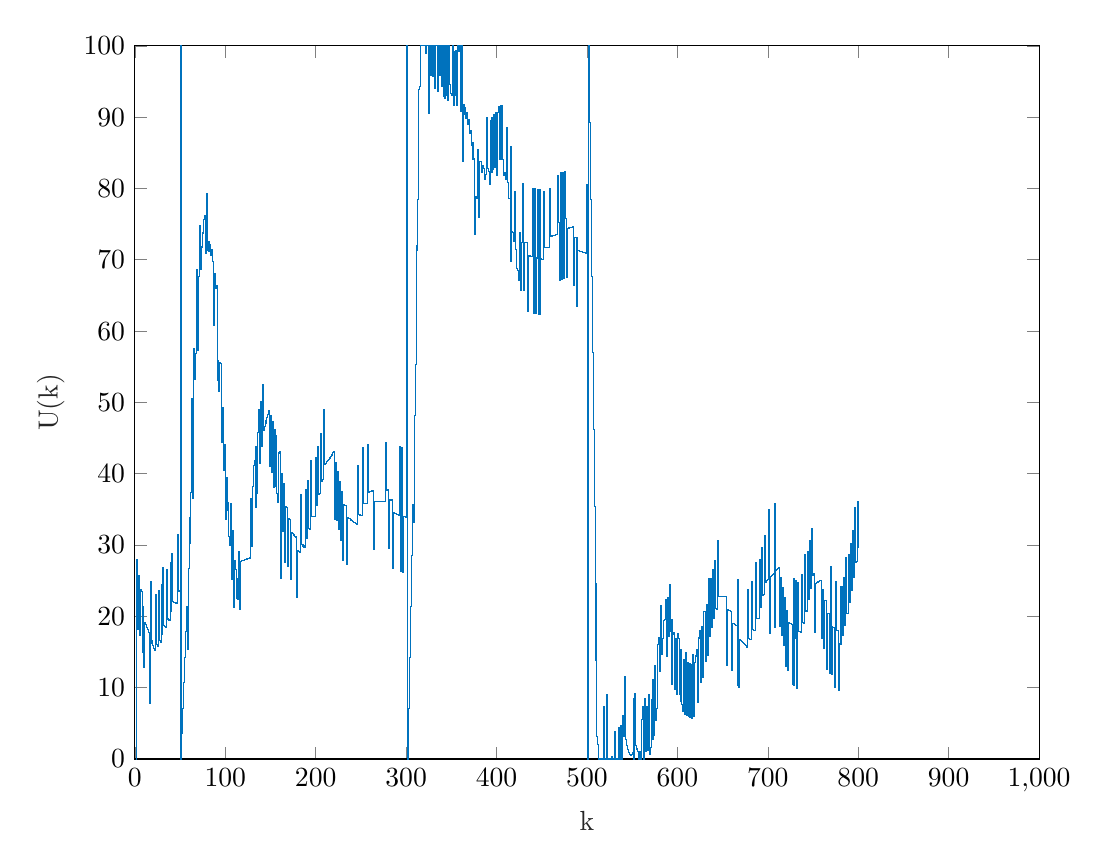
\begin{tikzpicture}

\begin{axis}[%
width=4.521in,
height=3.566in,
at={(0.758in,0.481in)},
scale only axis,
xmin=0,
xmax=1000,
xlabel style={font=\color{white!15!black}},
xlabel={k},
ymin=0,
ymax=100,
ylabel style={font=\color{white!15!black}},
ylabel={U(k)},
axis background/.style={fill=white}
]
\addplot[const plot, color=mycolor1, forget plot] table[row sep=crcr] {%
1	0\\
2	27.946429\\
3	18.117857\\
4	25.764286\\
5	17.264286\\
6	23.742857\\
7	23.471429\\
8	14.928571\\
9	21.364286\\
10	12.778571\\
11	19.171429\\
12	18.814286\\
13	18.457143\\
14	18.1\\
15	17.742857\\
16	7.735714\\
17	24.853571\\
18	16.621429\\
19	16.264286\\
20	15.907143\\
21	15.55\\
22	15.192857\\
23	23.107143\\
24	16.042857\\
25	15.728571\\
26	23.685714\\
27	16.664286\\
28	16.392857\\
29	24.392857\\
30	17.414286\\
31	26.835714\\
32	18.782143\\
33	18.603571\\
34	18.425\\
35	26.517857\\
36	19.632143\\
37	19.496429\\
38	19.360714\\
39	27.496429\\
40	20.653571\\
41	28.832143\\
42	22.032143\\
43	21.982143\\
44	21.932143\\
45	21.882143\\
46	21.832143\\
47	31.432143\\
48	23.557143\\
49	23.557143\\
50	100\\
51	0\\
52	3.571429\\
53	7.142857\\
54	10.714286\\
55	14.285714\\
56	17.857143\\
57	21.428571\\
58	15.35\\
59	26.746429\\
60	30.267857\\
61	33.789286\\
62	37.310714\\
63	50.482143\\
64	36.528571\\
65	57.575\\
66	53.271429\\
67	56.842857\\
68	68.685714\\
69	57.278571\\
70	67.6\\
71	71.171429\\
72	74.742857\\
73	68.664286\\
74	71.789286\\
75	73.746429\\
76	75.660714\\
77	76.153571\\
78	70.828571\\
79	79.314286\\
80	71.357143\\
81	72.560714\\
82	71.175\\
83	72.2\\
84	70.635714\\
85	71.482143\\
86	69.739286\\
87	60.757143\\
88	68.039286\\
89	65.982143\\
90	66.335714\\
91	55.828571\\
92	53.060714\\
93	51.535714\\
94	55.65\\
95	55.425\\
96	44.339286\\
97	49.264286\\
98	40.453571\\
99	44.032143\\
100	33.621429\\
101	39.475\\
102	35.989286\\
103	34.914286\\
104	31.25\\
105	29.996429\\
106	35.803571\\
107	25.167857\\
108	31.964286\\
109	21.192857\\
110	27.853571\\
111	26.596429\\
112	25.296429\\
113	22.575\\
114	22.307143\\
115	29.142857\\
116	20.957143\\
117	27.75\\
118	27.792857\\
119	27.835714\\
120	27.878571\\
121	27.921429\\
122	27.964286\\
123	28.007143\\
124	28.05\\
125	28.092857\\
126	28.135714\\
127	28.178571\\
128	36.492857\\
129	29.828571\\
130	38.185714\\
131	41.214286\\
132	41.789286\\
133	35.260714\\
134	43.753571\\
135	37.267857\\
136	45.803571\\
137	49.010714\\
138	41.492857\\
139	50.121429\\
140	43.771429\\
141	52.442857\\
142	46.135714\\
143	46.578571\\
144	47.021429\\
145	47.464286\\
146	47.907143\\
147	48.35\\
148	48.792857\\
149	40.964286\\
150	48.114286\\
151	40.242857\\
152	47.35\\
153	38.057143\\
154	46.239286\\
155	38.275\\
156	45.289286\\
157	37.282143\\
158	35.982143\\
159	42.910714\\
160	43.089286\\
161	25.346429\\
162	40.057143\\
163	31.871429\\
164	38.664286\\
165	30.435714\\
166	27.535714\\
167	35.360714\\
168	35.310714\\
169	26.989286\\
170	33.646429\\
171	33.553571\\
172	25.189286\\
173	31.803571\\
174	31.667857\\
175	31.532143\\
176	31.396429\\
177	31.260714\\
178	31.125\\
179	22.717857\\
180	29.289286\\
181	29.110714\\
182	28.932143\\
183	37.025\\
184	30.139286\\
185	30.003571\\
186	29.867857\\
187	29.732143\\
188	29.596429\\
189	37.732143\\
190	30.889286\\
191	39.067857\\
192	32.267857\\
193	32.217857\\
194	41.817857\\
195	33.942857\\
196	33.942857\\
197	33.942857\\
198	33.942857\\
199	33.942857\\
200	42.214286\\
201	35.507143\\
202	43.821429\\
203	37.157143\\
204	37.242857\\
205	45.6\\
206	38.978571\\
207	39.107143\\
208	39.235714\\
209	49.014286\\
210	41.317857\\
211	41.496429\\
212	41.675\\
213	41.853571\\
214	42.032143\\
215	42.210714\\
216	42.389286\\
217	42.567857\\
218	42.746429\\
219	42.925\\
220	43.103571\\
221	33.632143\\
222	41.635714\\
223	33.492857\\
224	40.328571\\
225	32.142857\\
226	38.935714\\
227	30.707143\\
228	37.457143\\
229	37.457143\\
230	27.807143\\
231	35.632143\\
232	35.582143\\
233	35.532143\\
234	27.210714\\
235	33.867857\\
236	33.775\\
237	33.682143\\
238	33.589286\\
239	33.496429\\
240	33.403571\\
241	33.310714\\
242	33.217857\\
243	33.125\\
244	33.032143\\
245	32.939286\\
246	41.117857\\
247	34.317857\\
248	34.267857\\
249	34.217857\\
250	34.167857\\
251	34.117857\\
252	43.717857\\
253	35.842857\\
254	35.842857\\
255	35.842857\\
256	35.842857\\
257	44.114286\\
258	37.407143\\
259	37.45\\
260	37.492857\\
261	37.535714\\
262	37.578571\\
263	37.621429\\
264	29.392857\\
265	36.142857\\
266	36.142857\\
267	36.142857\\
268	36.142857\\
269	36.142857\\
270	36.142857\\
271	36.142857\\
272	36.142857\\
273	36.142857\\
274	36.142857\\
275	36.142857\\
276	36.142857\\
277	44.414286\\
278	37.707143\\
279	37.75\\
280	37.792857\\
281	29.564286\\
282	36.314286\\
283	36.314286\\
284	36.314286\\
285	26.664286\\
286	34.489286\\
287	34.439286\\
288	34.389286\\
289	34.339286\\
290	34.289286\\
291	34.239286\\
292	34.189286\\
293	43.789286\\
294	26.264286\\
295	43.739286\\
296	26.214286\\
297	34.039286\\
298	33.989286\\
299	33.939286\\
300	33.889286\\
301	100\\
302	0\\
303	7.142857\\
304	14.285714\\
305	21.428571\\
306	28.571429\\
307	35.714286\\
308	33.207143\\
309	48.175\\
310	55.267857\\
311	72.010714\\
312	71.278571\\
313	78.421429\\
314	93.835714\\
315	94.271429\\
316	100\\
317	100\\
318	100\\
319	100\\
320	100\\
321	100\\
322	98.914286\\
323	100\\
324	100\\
325	90.55\\
326	100\\
327	95.792857\\
328	100\\
329	95.657143\\
330	100\\
331	93.957143\\
332	100\\
333	100\\
334	100\\
335	93.557143\\
336	100\\
337	95.832143\\
338	100\\
339	94.232143\\
340	100\\
341	92.885714\\
342	100\\
343	92.664286\\
344	93.067857\\
345	100\\
346	92.307143\\
347	100\\
348	94.582143\\
349	93.282143\\
350	92.971429\\
351	100\\
352	91.592857\\
353	99.196429\\
354	93.064286\\
355	99.321429\\
356	91.589286\\
357	100\\
358	99.192857\\
359	100\\
360	90.742857\\
361	100\\
362	83.814286\\
363	91.767857\\
364	90.382143\\
365	91.407143\\
366	89.842857\\
367	90.689286\\
368	88.946429\\
369	89.614286\\
370	87.692857\\
371	88.182143\\
372	86.082143\\
373	86.392857\\
374	84.114286\\
375	84.246429\\
376	73.517857\\
377	78.8\\
378	78.617857\\
379	85.496429\\
380	75.932143\\
381	83.8\\
382	83.75\\
383	82.278571\\
384	83.260714\\
385	83.075\\
386	82.846429\\
387	81.196429\\
388	82\\
389	89.907143\\
390	82.792857\\
391	82.385714\\
392	80.557143\\
393	89.453571\\
394	82.203571\\
395	89.932143\\
396	82.639286\\
397	90.325\\
398	82.989286\\
399	90.632143\\
400	81.875\\
401	90.592857\\
402	91.435714\\
403	84.007143\\
404	91.557143\\
405	84.085714\\
406	91.592857\\
407	84.078571\\
408	81.892857\\
409	82.160714\\
410	81.260714\\
411	88.589286\\
412	80.896429\\
413	78.532143\\
414	78.621429\\
415	85.814286\\
416	69.714286\\
417	73.921429\\
418	73.832143\\
419	72.575\\
420	79.546429\\
421	71.496429\\
422	68.775\\
423	68.507143\\
424	67.071429\\
425	73.864286\\
426	65.635714\\
427	72.385714\\
428	72.385714\\
429	80.657143\\
430	65.678571\\
431	72.428571\\
432	72.428571\\
433	72.428571\\
434	62.778571\\
435	70.603571\\
436	70.553571\\
437	70.503571\\
438	70.453571\\
439	70.403571\\
440	80.003571\\
441	62.478571\\
442	79.953571\\
443	62.428571\\
444	70.253571\\
445	79.853571\\
446	62.328571\\
447	79.803571\\
448	62.278571\\
449	70.103571\\
450	70.053571\\
451	70.003571\\
452	79.603571\\
453	71.728571\\
454	71.728571\\
455	71.728571\\
456	71.728571\\
457	71.728571\\
458	71.728571\\
459	80\\
460	73.292857\\
461	73.335714\\
462	73.378571\\
463	73.421429\\
464	73.464286\\
465	73.507143\\
466	73.55\\
467	81.864286\\
468	75.2\\
469	75.285714\\
470	67.1\\
471	82.164286\\
472	67.228571\\
473	82.292857\\
474	67.357143\\
475	82.421429\\
476	75.757143\\
477	67.571429\\
478	74.364286\\
479	74.407143\\
480	74.45\\
481	74.492857\\
482	74.535714\\
483	74.578571\\
484	74.621429\\
485	66.392857\\
486	73.142857\\
487	73.142857\\
488	73.142857\\
489	63.492857\\
490	71.317857\\
491	71.267857\\
492	71.217857\\
493	71.167857\\
494	71.117857\\
495	71.067857\\
496	71.017857\\
497	70.967857\\
498	70.917857\\
499	80.517857\\
500	72.642857\\
501	0\\
502	100\\
503	89.235714\\
504	78.471429\\
505	67.707143\\
506	56.942857\\
507	46.178571\\
508	35.414286\\
509	24.65\\
510	13.885714\\
511	3.121429\\
512	2.007143\\
513	0\\
514	0\\
515	0\\
516	0\\
517	0\\
518	7.292857\\
519	0\\
520	0\\
521	0\\
522	9.035714\\
523	0\\
524	0.010714\\
525	0\\
526	0\\
527	0.367857\\
528	0\\
529	0\\
530	0\\
531	3.803571\\
532	0\\
533	0\\
534	0\\
535	4.382143\\
536	0\\
537	4.696429\\
538	0\\
539	6.128571\\
540	4.560714\\
541	3.171429\\
542	11.610714\\
543	2.753571\\
544	1.95\\
545	1.325\\
546	0.878571\\
547	0.610714\\
548	0.521429\\
549	0.610714\\
550	0.878571\\
551	0\\
552	8.45\\
553	9.203571\\
554	1.864286\\
555	1.410714\\
556	1.092857\\
557	0\\
558	1.071429\\
559	0\\
560	5.546429\\
561	6.975\\
562	7.414286\\
563	0\\
564	8.535714\\
565	1.060714\\
566	7.321429\\
567	1.192857\\
568	9.053571\\
569	0.65\\
570	1.585714\\
571	8.382143\\
572	2.789286\\
573	11.185714\\
574	3.317857\\
575	13.060714\\
576	5.414286\\
577	7.107143\\
578	16.039286\\
579	16.978571\\
580	12.278571\\
581	21.567857\\
582	14.592857\\
583	16.957143\\
584	16.910714\\
585	19.453571\\
586	19.585714\\
587	22.307143\\
588	14.346429\\
589	22.575\\
590	17.246429\\
591	24.485714\\
592	17.914286\\
593	19.514286\\
594	10.389286\\
595	17.410714\\
596	17.725\\
597	9.810714\\
598	16.917857\\
599	9.046429\\
600	17.575\\
601	16.9\\
602	9.121429\\
603	8.092857\\
604	15.335714\\
605	7.6\\
606	6.614286\\
607	13.9\\
608	6.207143\\
609	14.914286\\
610	6.146429\\
611	13.525\\
612	5.925\\
613	13.346429\\
614	5.789286\\
615	13.253571\\
616	5.739286\\
617	14.625\\
618	6.035714\\
619	13.592857\\
620	14.442857\\
621	15.335714\\
622	8\\
623	17.064286\\
624	16.925\\
625	17.953571\\
626	10.753571\\
627	18.575\\
628	11.417857\\
629	20.660714\\
630	20.7\\
631	13.635714\\
632	21.592857\\
633	14.571429\\
634	22.571429\\
635	25.242857\\
636	17.189286\\
637	25.282143\\
638	18.396429\\
639	26.532143\\
640	19.689286\\
641	27.867857\\
642	21.067857\\
643	21.017857\\
644	30.617857\\
645	22.742857\\
646	22.742857\\
647	22.742857\\
648	22.742857\\
649	22.742857\\
650	22.742857\\
651	22.742857\\
652	22.742857\\
653	22.742857\\
654	13.092857\\
655	20.917857\\
656	20.867857\\
657	20.817857\\
658	20.767857\\
659	20.717857\\
660	12.396429\\
661	19.053571\\
662	18.960714\\
663	18.867857\\
664	18.775\\
665	18.682143\\
666	10.317857\\
667	25.203571\\
668	10.089286\\
669	16.703571\\
670	16.567857\\
671	16.432143\\
672	16.296429\\
673	16.160714\\
674	16.025\\
675	15.889286\\
676	15.753571\\
677	15.617857\\
678	23.753571\\
679	16.910714\\
680	16.817857\\
681	16.725\\
682	24.903571\\
683	18.103571\\
684	18.053571\\
685	18.003571\\
686	27.603571\\
687	19.728571\\
688	19.728571\\
689	19.728571\\
690	19.728571\\
691	28\\
692	21.292857\\
693	29.607143\\
694	22.942857\\
695	23.028571\\
696	31.385714\\
697	24.764286\\
698	24.892857\\
699	25.021429\\
700	25.15\\
701	34.928571\\
702	17.582143\\
703	25.585714\\
704	25.714286\\
705	25.842857\\
706	25.971429\\
707	35.75\\
708	18.403571\\
709	26.407143\\
710	26.535714\\
711	26.664286\\
712	26.792857\\
713	18.65\\
714	25.485714\\
715	17.3\\
716	24.092857\\
717	15.864286\\
718	22.614286\\
719	22.614286\\
720	12.964286\\
721	20.789286\\
722	12.467857\\
723	19.125\\
724	19.032143\\
725	18.939286\\
726	18.846429\\
727	10.482143\\
728	25.367857\\
729	10.253571\\
730	16.867857\\
731	25.003571\\
732	9.889286\\
733	24.775\\
734	17.932143\\
735	17.839286\\
736	17.746429\\
737	25.925\\
738	19.125\\
739	19.075\\
740	19.025\\
741	28.625\\
742	20.75\\
743	20.75\\
744	29.021429\\
745	22.314286\\
746	30.628571\\
747	23.964286\\
748	32.321429\\
749	25.7\\
750	25.828571\\
751	25.957143\\
752	17.814286\\
753	24.65\\
754	24.735714\\
755	24.821429\\
756	24.907143\\
757	24.992857\\
758	25.078571\\
759	16.892857\\
760	23.685714\\
761	23.728571\\
762	15.5\\
763	22.25\\
764	22.25\\
765	12.6\\
766	20.425\\
767	20.375\\
768	12.053571\\
769	26.982143\\
770	11.910714\\
771	18.567857\\
772	18.475\\
773	18.382143\\
774	10.017857\\
775	24.903571\\
776	18.060714\\
777	17.967857\\
778	9.603571\\
779	16.217857\\
780	16.082143\\
781	24.217857\\
782	17.375\\
783	17.282143\\
784	25.460714\\
785	18.660714\\
786	28.260714\\
787	20.385714\\
788	20.385714\\
789	28.657143\\
790	21.95\\
791	30.264286\\
792	23.6\\
793	23.685714\\
794	32.042857\\
795	25.421429\\
796	35.2\\
797	27.503571\\
798	27.682143\\
799	36.132143\\
800	29.603571\\
};
\end{axis}
\end{tikzpicture}%
\caption{Sterowanie dla rozmytego PID}
\end{figure}

Wartość wskaźnika jakości:

\begin{equation}
E = 22,9549e+07
\end{equation}

Wyniki działania regulacji dla następujących nastaw regulatorów lokalnych:

Regulator lokalny PID 1
\begin{equation}
K = 21; 
T_i = 60; 
T_d = 0; 
\end{equation}

Regulator lokalny PID 2
\begin{equation}
K = 15; 
T_i = 50; 
T_d = 0; 
\end{equation}

Regulator lokalny PID 3
\begin{equation}
K = 21; 
T_i = 55; 
T_d = 0; 
\end{equation}

\begin{figure}[H]
\centering
% This file was created by matlab2tikz.
%
%The latest updates can be retrieved from
%  http://www.mathworks.com/matlabcentral/fileexchange/22022-matlab2tikz-matlab2tikz
%where you can also make suggestions and rate matlab2tikz.
%
\definecolor{mycolor1}{rgb}{0.00000,0.44700,0.74100}%
%
\begin{tikzpicture}

\begin{axis}[%
width=4.521in,
height=3.566in,
at={(0.758in,0.481in)},
scale only axis,
xmin=0,
xmax=1000,
xlabel style={font=\color{white!15!black}},
xlabel={k},
ymin=30,
ymax=46,
ylabel style={font=\color{white!15!black}},
ylabel={Y(k)},
axis background/.style={fill=white}
]
\addplot[const plot, color=mycolor1, forget plot] table[row sep=crcr] {%
1	32.18\\
2	32.18\\
3	32.18\\
4	32.25\\
5	32.18\\
6	32.18\\
7	32.25\\
8	32.18\\
9	32.18\\
10	32.18\\
11	32.18\\
12	32.18\\
13	32.18\\
14	32.12\\
15	32.12\\
16	32.06\\
17	32\\
18	31.93\\
19	31.87\\
20	31.81\\
21	31.68\\
22	31.62\\
23	31.56\\
24	31.43\\
25	31.31\\
26	31.25\\
27	31.12\\
28	31.06\\
29	31\\
30	30.87\\
31	30.81\\
32	30.68\\
33	30.62\\
34	30.56\\
35	30.5\\
36	30.43\\
37	30.37\\
38	30.31\\
39	30.31\\
40	30.25\\
41	30.25\\
42	30.18\\
43	30.18\\
44	30.18\\
45	30.18\\
46	30.18\\
47	30.18\\
48	30.25\\
49	30.25\\
50	30.31\\
51	30.31\\
52	30.37\\
53	30.43\\
54	30.5\\
55	30.56\\
56	30.62\\
57	30.68\\
58	30.81\\
59	30.93\\
60	31.06\\
61	31.12\\
62	31.31\\
63	31.5\\
64	31.62\\
65	31.81\\
66	32\\
67	32.18\\
68	32.37\\
69	32.62\\
70	32.81\\
71	33\\
72	33.18\\
73	33.43\\
74	33.62\\
75	33.87\\
76	34.06\\
77	34.25\\
78	34.5\\
79	35.12\\
80	35.31\\
81	35.5\\
82	35.68\\
83	35.87\\
84	36\\
85	36.18\\
86	36.31\\
87	36.43\\
88	36.56\\
89	36.68\\
90	36.75\\
91	36.81\\
92	36.87\\
93	37\\
94	37\\
95	37\\
96	37\\
97	37\\
98	36.93\\
99	36.93\\
100	36.87\\
101	36.81\\
102	36.81\\
103	36.75\\
104	36.62\\
105	36.56\\
106	36.43\\
107	36.37\\
108	36.25\\
109	36.12\\
110	36\\
111	35.93\\
112	35.81\\
113	35.68\\
114	35.62\\
115	35.5\\
116	35.37\\
117	35.25\\
118	35.18\\
119	35.12\\
120	35\\
121	34.93\\
122	34.81\\
123	34.75\\
124	34.68\\
125	34.62\\
126	34.56\\
127	34.5\\
128	34.43\\
129	34.43\\
130	34.37\\
131	34.31\\
132	34.31\\
133	34.31\\
134	34.31\\
135	34.37\\
136	34.37\\
137	34.37\\
138	34.43\\
139	34.5\\
140	34.56\\
141	34.62\\
142	34.68\\
143	34.75\\
144	34.81\\
145	34.87\\
146	35\\
147	35.06\\
148	35.18\\
149	35.25\\
150	35.37\\
151	35.43\\
152	35.56\\
153	35.68\\
154	35.75\\
155	35.87\\
156	36\\
157	36.06\\
158	36.12\\
159	36.25\\
160	36.31\\
161	36.37\\
162	36.43\\
163	36.5\\
164	36.56\\
165	36.62\\
166	36.68\\
167	36.68\\
168	36.75\\
169	36.75\\
170	36.75\\
171	36.81\\
172	36.81\\
173	36.81\\
174	36.81\\
175	36.81\\
176	36.81\\
177	36.81\\
178	36.75\\
179	36.75\\
180	36.68\\
181	36.68\\
182	36.56\\
183	36.56\\
184	36.5\\
185	36.43\\
186	36.43\\
187	36.43\\
188	36.37\\
189	36.37\\
190	36.31\\
191	36.25\\
192	36.18\\
193	36.12\\
194	36.06\\
195	36\\
196	35.93\\
197	35.87\\
198	35.81\\
199	35.68\\
200	35.68\\
201	35.62\\
202	35.62\\
203	35.56\\
204	35.5\\
205	35.5\\
206	35.43\\
207	35.37\\
208	35.37\\
209	35.31\\
210	35.31\\
211	35.31\\
212	35.31\\
213	35.31\\
214	35.31\\
215	35.31\\
216	35.37\\
217	35.37\\
218	35.43\\
219	35.43\\
220	35.5\\
221	35.5\\
222	35.56\\
223	35.62\\
224	35.68\\
225	35.75\\
226	35.75\\
227	35.81\\
228	35.87\\
229	35.87\\
230	35.93\\
231	36\\
232	36.06\\
233	36.12\\
234	36.12\\
235	36.18\\
236	36.18\\
237	36.18\\
238	36.25\\
239	36.25\\
240	36.25\\
241	36.31\\
242	36.31\\
243	36.31\\
244	36.31\\
245	36.31\\
246	36.25\\
247	36.25\\
248	36.25\\
249	36.25\\
250	36.25\\
251	36.25\\
252	36.25\\
253	36.25\\
254	36.25\\
255	36.25\\
256	36.25\\
257	36.25\\
258	36.25\\
259	36.25\\
260	36.25\\
261	36.25\\
262	36.25\\
263	36.25\\
264	36.25\\
265	36.18\\
266	36.18\\
267	36.18\\
268	36.12\\
269	36.12\\
270	36.12\\
271	36.12\\
272	36.12\\
273	36.12\\
274	36.06\\
275	36.06\\
276	36.06\\
277	36\\
278	36\\
279	35.93\\
280	35.93\\
281	35.93\\
282	35.93\\
283	35.93\\
284	35.93\\
285	35.93\\
286	35.93\\
287	35.93\\
288	35.93\\
289	35.87\\
290	35.87\\
291	35.87\\
292	35.87\\
293	35.87\\
294	35.87\\
295	35.87\\
296	35.87\\
297	35.87\\
298	35.87\\
299	35.87\\
300	35.87\\
301	35.87\\
302	35.87\\
303	35.87\\
304	35.93\\
305	35.93\\
306	35.93\\
307	35.93\\
308	35.93\\
309	36\\
310	36\\
311	36.06\\
312	36.12\\
313	36.18\\
314	36.31\\
315	36.43\\
316	36.56\\
317	36.62\\
318	36.75\\
319	36.93\\
320	37.06\\
321	37.18\\
322	37.31\\
323	37.43\\
324	37.62\\
325	37.81\\
326	38\\
327	38.12\\
328	38.31\\
329	38.56\\
330	38.68\\
331	38.87\\
332	39\\
333	39.18\\
334	39.37\\
335	39.56\\
336	39.68\\
337	39.87\\
338	40.06\\
339	40.18\\
340	40.37\\
341	40.5\\
342	40.68\\
343	40.81\\
344	40.93\\
345	41.12\\
346	41.25\\
347	41.37\\
348	41.5\\
349	41.62\\
350	41.75\\
351	41.81\\
352	41.93\\
353	42.06\\
354	42.18\\
355	42.31\\
356	42.43\\
357	42.5\\
358	42.62\\
359	42.68\\
360	42.81\\
361	42.87\\
362	42.93\\
363	43\\
364	43.06\\
365	43.12\\
366	43.18\\
367	43.31\\
368	43.31\\
369	43.37\\
370	43.43\\
371	43.43\\
372	43.5\\
373	43.5\\
374	43.56\\
375	43.56\\
376	43.56\\
377	43.56\\
378	43.62\\
379	43.68\\
380	43.68\\
381	43.68\\
382	43.68\\
383	43.68\\
384	43.68\\
385	43.68\\
386	43.62\\
387	43.62\\
388	43.62\\
389	43.62\\
390	43.62\\
391	43.62\\
392	43.62\\
393	43.68\\
394	43.68\\
395	43.75\\
396	43.75\\
397	43.81\\
398	43.81\\
399	43.81\\
400	43.81\\
401	43.87\\
402	43.87\\
403	44\\
404	44\\
405	44\\
406	44\\
407	44\\
408	44.06\\
409	44.06\\
410	44.12\\
411	44.18\\
412	44.18\\
413	44.25\\
414	44.25\\
415	44.25\\
416	44.31\\
417	44.31\\
418	44.37\\
419	44.37\\
420	44.43\\
421	44.43\\
422	44.5\\
423	44.56\\
424	44.56\\
425	44.62\\
426	44.62\\
427	44.68\\
428	44.75\\
429	44.81\\
430	44.87\\
431	44.93\\
432	45\\
433	45.06\\
434	45.12\\
435	45.18\\
436	45.31\\
437	45.37\\
438	45.43\\
439	45.5\\
440	45.56\\
441	45.62\\
442	45.68\\
443	45.75\\
444	45.81\\
445	45.81\\
446	45.81\\
447	45.87\\
448	45.87\\
449	45.87\\
450	45.87\\
451	45.87\\
452	45.87\\
453	45.87\\
454	45.93\\
455	45.93\\
456	45.87\\
457	45.81\\
458	45.81\\
459	45.81\\
460	45.75\\
461	45.75\\
462	45.75\\
463	45.68\\
464	45.68\\
465	45.68\\
466	45.68\\
467	45.62\\
468	45.62\\
469	45.62\\
470	45.62\\
471	45.62\\
472	45.62\\
473	45.56\\
474	45.56\\
475	45.56\\
476	45.56\\
477	45.56\\
478	45.56\\
479	45.56\\
480	45.56\\
481	45.56\\
482	45.56\\
483	45.56\\
484	45.56\\
485	45.5\\
486	45.56\\
487	45.5\\
488	45.56\\
489	45.5\\
490	45.5\\
491	45.5\\
492	45.5\\
493	45.5\\
494	45.43\\
495	45.43\\
496	45.43\\
497	45.5\\
498	45.5\\
499	45.5\\
500	45.5\\
501	45.56\\
502	45.62\\
503	45.62\\
504	45.62\\
505	45.68\\
506	45.68\\
507	45.68\\
508	45.68\\
509	45.62\\
510	45.62\\
511	45.56\\
512	45.43\\
513	45.37\\
514	45.25\\
515	45.12\\
516	45\\
517	44.81\\
518	44.68\\
519	44.5\\
520	44.31\\
521	44.06\\
522	43.87\\
523	43.62\\
524	43.37\\
525	43.12\\
526	42.87\\
527	42.62\\
528	42.43\\
529	42.12\\
530	41.87\\
531	41.62\\
532	41.43\\
533	41.12\\
534	40.93\\
535	40.68\\
536	40.43\\
537	40.18\\
538	39.93\\
539	39.75\\
540	39.5\\
541	39.25\\
542	39.06\\
543	38.87\\
544	38.75\\
545	38.56\\
546	38.37\\
547	38.25\\
548	38.06\\
549	37.87\\
550	37.75\\
551	37.62\\
552	37.5\\
553	37.37\\
554	37.31\\
555	37.18\\
556	37.12\\
557	37.06\\
558	37\\
559	36.93\\
560	36.87\\
561	36.81\\
562	36.75\\
563	36.75\\
564	36.68\\
565	36.68\\
566	36.62\\
567	36.62\\
568	36.62\\
569	36.56\\
570	36.56\\
571	36.56\\
572	36.5\\
573	36.5\\
574	36.5\\
575	36.43\\
576	36.37\\
577	36.37\\
578	36.31\\
579	36.25\\
580	36.25\\
581	36.18\\
582	36.12\\
583	36.06\\
584	36\\
585	35.93\\
586	35.81\\
587	35.75\\
588	35.68\\
589	35.56\\
590	35.43\\
591	35.37\\
592	35.25\\
593	35.12\\
594	35\\
595	34.87\\
596	34.75\\
597	34.62\\
598	34.5\\
599	34.37\\
600	34.25\\
601	34.12\\
602	34\\
603	33.87\\
604	33.75\\
605	33.62\\
606	33.5\\
607	33.37\\
608	33.31\\
609	33.18\\
610	33.06\\
611	33\\
612	32.87\\
613	32.81\\
614	32.75\\
615	32.68\\
616	32.62\\
617	32.56\\
618	32.56\\
619	32.5\\
620	32.5\\
621	32.5\\
622	32.5\\
623	32.5\\
624	32.5\\
625	32.5\\
626	32.56\\
627	32.56\\
628	32.62\\
629	32.62\\
630	32.68\\
631	32.68\\
632	32.75\\
633	32.81\\
634	32.81\\
635	32.87\\
636	32.87\\
637	32.93\\
638	32.93\\
639	32.93\\
640	32.93\\
641	33\\
642	33\\
643	33.06\\
644	33.06\\
645	33.06\\
646	33.06\\
647	33\\
648	33\\
649	33\\
650	33\\
651	33\\
652	33\\
653	32.93\\
654	32.87\\
655	32.81\\
656	32.75\\
657	32.75\\
658	32.68\\
659	32.56\\
660	32.5\\
661	32.43\\
662	32.37\\
663	32.31\\
664	32.25\\
665	32.12\\
666	32.06\\
667	31.93\\
668	31.87\\
669	31.75\\
670	31.68\\
671	31.62\\
672	31.56\\
673	31.5\\
674	31.43\\
675	31.37\\
676	31.31\\
677	31.25\\
678	31.18\\
679	31.18\\
680	31.12\\
681	31.06\\
682	31.06\\
683	31\\
684	31\\
685	31\\
686	30.93\\
687	31\\
688	31\\
689	31\\
690	31\\
691	31.06\\
692	31.06\\
693	31.12\\
694	31.12\\
695	31.12\\
696	31.18\\
697	31.18\\
698	31.31\\
699	31.31\\
700	31.37\\
701	31.43\\
702	31.5\\
703	31.5\\
704	31.56\\
705	31.62\\
706	31.68\\
707	31.68\\
708	31.75\\
709	31.75\\
710	31.81\\
711	31.81\\
712	31.81\\
713	31.87\\
714	31.87\\
715	31.93\\
716	31.93\\
717	31.93\\
718	31.93\\
719	31.93\\
720	31.93\\
721	31.93\\
722	31.87\\
723	31.87\\
724	31.81\\
725	31.75\\
726	31.75\\
727	31.68\\
728	31.62\\
729	31.62\\
730	31.56\\
731	31.5\\
732	31.43\\
733	31.43\\
734	31.37\\
735	31.31\\
736	31.25\\
737	31.18\\
738	31.12\\
739	31.06\\
740	30.93\\
741	30.87\\
742	30.87\\
743	30.81\\
744	30.75\\
745	30.75\\
746	30.68\\
747	30.68\\
748	30.62\\
749	30.62\\
750	30.56\\
751	30.56\\
752	30.56\\
753	30.56\\
754	30.56\\
755	30.56\\
756	30.56\\
757	30.56\\
758	30.56\\
759	30.62\\
760	30.62\\
761	30.62\\
762	30.68\\
763	30.75\\
764	30.81\\
765	30.81\\
766	30.87\\
767	30.93\\
768	30.93\\
769	31\\
770	31.06\\
771	31.12\\
772	31.12\\
773	31.18\\
774	31.25\\
775	31.25\\
776	31.31\\
777	31.37\\
778	31.37\\
779	31.43\\
780	31.43\\
781	31.5\\
782	31.5\\
783	31.5\\
784	31.56\\
785	31.56\\
786	31.56\\
787	31.5\\
788	31.56\\
789	31.5\\
790	31.5\\
791	31.5\\
792	31.5\\
793	31.43\\
794	31.43\\
795	31.43\\
796	31.37\\
797	31.37\\
798	31.31\\
799	31.25\\
800	31.25\\
801	31.18\\
};
\addplot [color=red, dashed, forget plot]
  table[row sep=crcr]{%
1	30.93\\
2	30.93\\
3	30.93\\
4	30.93\\
5	30.93\\
6	30.93\\
7	30.93\\
8	30.93\\
9	30.93\\
10	30.93\\
11	30.93\\
12	30.93\\
13	30.93\\
14	30.93\\
15	30.93\\
16	30.93\\
17	30.93\\
18	30.93\\
19	30.93\\
20	30.93\\
21	30.93\\
22	30.93\\
23	30.93\\
24	30.93\\
25	30.93\\
26	30.93\\
27	30.93\\
28	30.93\\
29	30.93\\
30	30.93\\
31	30.93\\
32	30.93\\
33	30.93\\
34	30.93\\
35	30.93\\
36	30.93\\
37	30.93\\
38	30.93\\
39	30.93\\
40	30.93\\
41	30.93\\
42	30.93\\
43	30.93\\
44	30.93\\
45	30.93\\
46	30.93\\
47	30.93\\
48	30.93\\
49	30.93\\
50	30.93\\
51	35.93\\
52	35.93\\
53	35.93\\
54	35.93\\
55	35.93\\
56	35.93\\
57	35.93\\
58	35.93\\
59	35.93\\
60	35.93\\
61	35.93\\
62	35.93\\
63	35.93\\
64	35.93\\
65	35.93\\
66	35.93\\
67	35.93\\
68	35.93\\
69	35.93\\
70	35.93\\
71	35.93\\
72	35.93\\
73	35.93\\
74	35.93\\
75	35.93\\
76	35.93\\
77	35.93\\
78	35.93\\
79	35.93\\
80	35.93\\
81	35.93\\
82	35.93\\
83	35.93\\
84	35.93\\
85	35.93\\
86	35.93\\
87	35.93\\
88	35.93\\
89	35.93\\
90	35.93\\
91	35.93\\
92	35.93\\
93	35.93\\
94	35.93\\
95	35.93\\
96	35.93\\
97	35.93\\
98	35.93\\
99	35.93\\
100	35.93\\
101	35.93\\
102	35.93\\
103	35.93\\
104	35.93\\
105	35.93\\
106	35.93\\
107	35.93\\
108	35.93\\
109	35.93\\
110	35.93\\
111	35.93\\
112	35.93\\
113	35.93\\
114	35.93\\
115	35.93\\
116	35.93\\
117	35.93\\
118	35.93\\
119	35.93\\
120	35.93\\
121	35.93\\
122	35.93\\
123	35.93\\
124	35.93\\
125	35.93\\
126	35.93\\
127	35.93\\
128	35.93\\
129	35.93\\
130	35.93\\
131	35.93\\
132	35.93\\
133	35.93\\
134	35.93\\
135	35.93\\
136	35.93\\
137	35.93\\
138	35.93\\
139	35.93\\
140	35.93\\
141	35.93\\
142	35.93\\
143	35.93\\
144	35.93\\
145	35.93\\
146	35.93\\
147	35.93\\
148	35.93\\
149	35.93\\
150	35.93\\
151	35.93\\
152	35.93\\
153	35.93\\
154	35.93\\
155	35.93\\
156	35.93\\
157	35.93\\
158	35.93\\
159	35.93\\
160	35.93\\
161	35.93\\
162	35.93\\
163	35.93\\
164	35.93\\
165	35.93\\
166	35.93\\
167	35.93\\
168	35.93\\
169	35.93\\
170	35.93\\
171	35.93\\
172	35.93\\
173	35.93\\
174	35.93\\
175	35.93\\
176	35.93\\
177	35.93\\
178	35.93\\
179	35.93\\
180	35.93\\
181	35.93\\
182	35.93\\
183	35.93\\
184	35.93\\
185	35.93\\
186	35.93\\
187	35.93\\
188	35.93\\
189	35.93\\
190	35.93\\
191	35.93\\
192	35.93\\
193	35.93\\
194	35.93\\
195	35.93\\
196	35.93\\
197	35.93\\
198	35.93\\
199	35.93\\
200	35.93\\
201	35.93\\
202	35.93\\
203	35.93\\
204	35.93\\
205	35.93\\
206	35.93\\
207	35.93\\
208	35.93\\
209	35.93\\
210	35.93\\
211	35.93\\
212	35.93\\
213	35.93\\
214	35.93\\
215	35.93\\
216	35.93\\
217	35.93\\
218	35.93\\
219	35.93\\
220	35.93\\
221	35.93\\
222	35.93\\
223	35.93\\
224	35.93\\
225	35.93\\
226	35.93\\
227	35.93\\
228	35.93\\
229	35.93\\
230	35.93\\
231	35.93\\
232	35.93\\
233	35.93\\
234	35.93\\
235	35.93\\
236	35.93\\
237	35.93\\
238	35.93\\
239	35.93\\
240	35.93\\
241	35.93\\
242	35.93\\
243	35.93\\
244	35.93\\
245	35.93\\
246	35.93\\
247	35.93\\
248	35.93\\
249	35.93\\
250	35.93\\
251	35.93\\
252	35.93\\
253	35.93\\
254	35.93\\
255	35.93\\
256	35.93\\
257	35.93\\
258	35.93\\
259	35.93\\
260	35.93\\
261	35.93\\
262	35.93\\
263	35.93\\
264	35.93\\
265	35.93\\
266	35.93\\
267	35.93\\
268	35.93\\
269	35.93\\
270	35.93\\
271	35.93\\
272	35.93\\
273	35.93\\
274	35.93\\
275	35.93\\
276	35.93\\
277	35.93\\
278	35.93\\
279	35.93\\
280	35.93\\
281	35.93\\
282	35.93\\
283	35.93\\
284	35.93\\
285	35.93\\
286	35.93\\
287	35.93\\
288	35.93\\
289	35.93\\
290	35.93\\
291	35.93\\
292	35.93\\
293	35.93\\
294	35.93\\
295	35.93\\
296	35.93\\
297	35.93\\
298	35.93\\
299	35.93\\
300	35.93\\
301	45.93\\
302	45.93\\
303	45.93\\
304	45.93\\
305	45.93\\
306	45.93\\
307	45.93\\
308	45.93\\
309	45.93\\
310	45.93\\
311	45.93\\
312	45.93\\
313	45.93\\
314	45.93\\
315	45.93\\
316	45.93\\
317	45.93\\
318	45.93\\
319	45.93\\
320	45.93\\
321	45.93\\
322	45.93\\
323	45.93\\
324	45.93\\
325	45.93\\
326	45.93\\
327	45.93\\
328	45.93\\
329	45.93\\
330	45.93\\
331	45.93\\
332	45.93\\
333	45.93\\
334	45.93\\
335	45.93\\
336	45.93\\
337	45.93\\
338	45.93\\
339	45.93\\
340	45.93\\
341	45.93\\
342	45.93\\
343	45.93\\
344	45.93\\
345	45.93\\
346	45.93\\
347	45.93\\
348	45.93\\
349	45.93\\
350	45.93\\
351	45.93\\
352	45.93\\
353	45.93\\
354	45.93\\
355	45.93\\
356	45.93\\
357	45.93\\
358	45.93\\
359	45.93\\
360	45.93\\
361	45.93\\
362	45.93\\
363	45.93\\
364	45.93\\
365	45.93\\
366	45.93\\
367	45.93\\
368	45.93\\
369	45.93\\
370	45.93\\
371	45.93\\
372	45.93\\
373	45.93\\
374	45.93\\
375	45.93\\
376	45.93\\
377	45.93\\
378	45.93\\
379	45.93\\
380	45.93\\
381	45.93\\
382	45.93\\
383	45.93\\
384	45.93\\
385	45.93\\
386	45.93\\
387	45.93\\
388	45.93\\
389	45.93\\
390	45.93\\
391	45.93\\
392	45.93\\
393	45.93\\
394	45.93\\
395	45.93\\
396	45.93\\
397	45.93\\
398	45.93\\
399	45.93\\
400	45.93\\
401	45.93\\
402	45.93\\
403	45.93\\
404	45.93\\
405	45.93\\
406	45.93\\
407	45.93\\
408	45.93\\
409	45.93\\
410	45.93\\
411	45.93\\
412	45.93\\
413	45.93\\
414	45.93\\
415	45.93\\
416	45.93\\
417	45.93\\
418	45.93\\
419	45.93\\
420	45.93\\
421	45.93\\
422	45.93\\
423	45.93\\
424	45.93\\
425	45.93\\
426	45.93\\
427	45.93\\
428	45.93\\
429	45.93\\
430	45.93\\
431	45.93\\
432	45.93\\
433	45.93\\
434	45.93\\
435	45.93\\
436	45.93\\
437	45.93\\
438	45.93\\
439	45.93\\
440	45.93\\
441	45.93\\
442	45.93\\
443	45.93\\
444	45.93\\
445	45.93\\
446	45.93\\
447	45.93\\
448	45.93\\
449	45.93\\
450	45.93\\
451	45.93\\
452	45.93\\
453	45.93\\
454	45.93\\
455	45.93\\
456	45.93\\
457	45.93\\
458	45.93\\
459	45.93\\
460	45.93\\
461	45.93\\
462	45.93\\
463	45.93\\
464	45.93\\
465	45.93\\
466	45.93\\
467	45.93\\
468	45.93\\
469	45.93\\
470	45.93\\
471	45.93\\
472	45.93\\
473	45.93\\
474	45.93\\
475	45.93\\
476	45.93\\
477	45.93\\
478	45.93\\
479	45.93\\
480	45.93\\
481	45.93\\
482	45.93\\
483	45.93\\
484	45.93\\
485	45.93\\
486	45.93\\
487	45.93\\
488	45.93\\
489	45.93\\
490	45.93\\
491	45.93\\
492	45.93\\
493	45.93\\
494	45.93\\
495	45.93\\
496	45.93\\
497	45.93\\
498	45.93\\
499	45.93\\
500	45.93\\
501	30.93\\
502	30.93\\
503	30.93\\
504	30.93\\
505	30.93\\
506	30.93\\
507	30.93\\
508	30.93\\
509	30.93\\
510	30.93\\
511	30.93\\
512	30.93\\
513	30.93\\
514	30.93\\
515	30.93\\
516	30.93\\
517	30.93\\
518	30.93\\
519	30.93\\
520	30.93\\
521	30.93\\
522	30.93\\
523	30.93\\
524	30.93\\
525	30.93\\
526	30.93\\
527	30.93\\
528	30.93\\
529	30.93\\
530	30.93\\
531	30.93\\
532	30.93\\
533	30.93\\
534	30.93\\
535	30.93\\
536	30.93\\
537	30.93\\
538	30.93\\
539	30.93\\
540	30.93\\
541	30.93\\
542	30.93\\
543	30.93\\
544	30.93\\
545	30.93\\
546	30.93\\
547	30.93\\
548	30.93\\
549	30.93\\
550	30.93\\
551	30.93\\
552	30.93\\
553	30.93\\
554	30.93\\
555	30.93\\
556	30.93\\
557	30.93\\
558	30.93\\
559	30.93\\
560	30.93\\
561	30.93\\
562	30.93\\
563	30.93\\
564	30.93\\
565	30.93\\
566	30.93\\
567	30.93\\
568	30.93\\
569	30.93\\
570	30.93\\
571	30.93\\
572	30.93\\
573	30.93\\
574	30.93\\
575	30.93\\
576	30.93\\
577	30.93\\
578	30.93\\
579	30.93\\
580	30.93\\
581	30.93\\
582	30.93\\
583	30.93\\
584	30.93\\
585	30.93\\
586	30.93\\
587	30.93\\
588	30.93\\
589	30.93\\
590	30.93\\
591	30.93\\
592	30.93\\
593	30.93\\
594	30.93\\
595	30.93\\
596	30.93\\
597	30.93\\
598	30.93\\
599	30.93\\
600	30.93\\
601	30.93\\
602	30.93\\
603	30.93\\
604	30.93\\
605	30.93\\
606	30.93\\
607	30.93\\
608	30.93\\
609	30.93\\
610	30.93\\
611	30.93\\
612	30.93\\
613	30.93\\
614	30.93\\
615	30.93\\
616	30.93\\
617	30.93\\
618	30.93\\
619	30.93\\
620	30.93\\
621	30.93\\
622	30.93\\
623	30.93\\
624	30.93\\
625	30.93\\
626	30.93\\
627	30.93\\
628	30.93\\
629	30.93\\
630	30.93\\
631	30.93\\
632	30.93\\
633	30.93\\
634	30.93\\
635	30.93\\
636	30.93\\
637	30.93\\
638	30.93\\
639	30.93\\
640	30.93\\
641	30.93\\
642	30.93\\
643	30.93\\
644	30.93\\
645	30.93\\
646	30.93\\
647	30.93\\
648	30.93\\
649	30.93\\
650	30.93\\
651	30.93\\
652	30.93\\
653	30.93\\
654	30.93\\
655	30.93\\
656	30.93\\
657	30.93\\
658	30.93\\
659	30.93\\
660	30.93\\
661	30.93\\
662	30.93\\
663	30.93\\
664	30.93\\
665	30.93\\
666	30.93\\
667	30.93\\
668	30.93\\
669	30.93\\
670	30.93\\
671	30.93\\
672	30.93\\
673	30.93\\
674	30.93\\
675	30.93\\
676	30.93\\
677	30.93\\
678	30.93\\
679	30.93\\
680	30.93\\
681	30.93\\
682	30.93\\
683	30.93\\
684	30.93\\
685	30.93\\
686	30.93\\
687	30.93\\
688	30.93\\
689	30.93\\
690	30.93\\
691	30.93\\
692	30.93\\
693	30.93\\
694	30.93\\
695	30.93\\
696	30.93\\
697	30.93\\
698	30.93\\
699	30.93\\
700	30.93\\
701	30.93\\
702	30.93\\
703	30.93\\
704	30.93\\
705	30.93\\
706	30.93\\
707	30.93\\
708	30.93\\
709	30.93\\
710	30.93\\
711	30.93\\
712	30.93\\
713	30.93\\
714	30.93\\
715	30.93\\
716	30.93\\
717	30.93\\
718	30.93\\
719	30.93\\
720	30.93\\
721	30.93\\
722	30.93\\
723	30.93\\
724	30.93\\
725	30.93\\
726	30.93\\
727	30.93\\
728	30.93\\
729	30.93\\
730	30.93\\
731	30.93\\
732	30.93\\
733	30.93\\
734	30.93\\
735	30.93\\
736	30.93\\
737	30.93\\
738	30.93\\
739	30.93\\
740	30.93\\
741	30.93\\
742	30.93\\
743	30.93\\
744	30.93\\
745	30.93\\
746	30.93\\
747	30.93\\
748	30.93\\
749	30.93\\
750	30.93\\
751	30.93\\
752	30.93\\
753	30.93\\
754	30.93\\
755	30.93\\
756	30.93\\
757	30.93\\
758	30.93\\
759	30.93\\
760	30.93\\
761	30.93\\
762	30.93\\
763	30.93\\
764	30.93\\
765	30.93\\
766	30.93\\
767	30.93\\
768	30.93\\
769	30.93\\
770	30.93\\
771	30.93\\
772	30.93\\
773	30.93\\
774	30.93\\
775	30.93\\
776	30.93\\
777	30.93\\
778	30.93\\
779	30.93\\
780	30.93\\
781	30.93\\
782	30.93\\
783	30.93\\
784	30.93\\
785	30.93\\
786	30.93\\
787	30.93\\
788	30.93\\
789	30.93\\
790	30.93\\
791	30.93\\
792	30.93\\
793	30.93\\
794	30.93\\
795	30.93\\
796	30.93\\
797	30.93\\
798	30.93\\
799	30.93\\
800	30.93\\
};
\end{axis}
\end{tikzpicture}%
\caption{Regulacja dla rozmytego PID}
\end{figure}

\begin{figure}[H]
\centering
% This file was created by matlab2tikz.
%
%The latest updates can be retrieved from
%  http://www.mathworks.com/matlabcentral/fileexchange/22022-matlab2tikz-matlab2tikz
%where you can also make suggestions and rate matlab2tikz.
%
\definecolor{mycolor1}{rgb}{0.00000,0.44700,0.74100}%
%
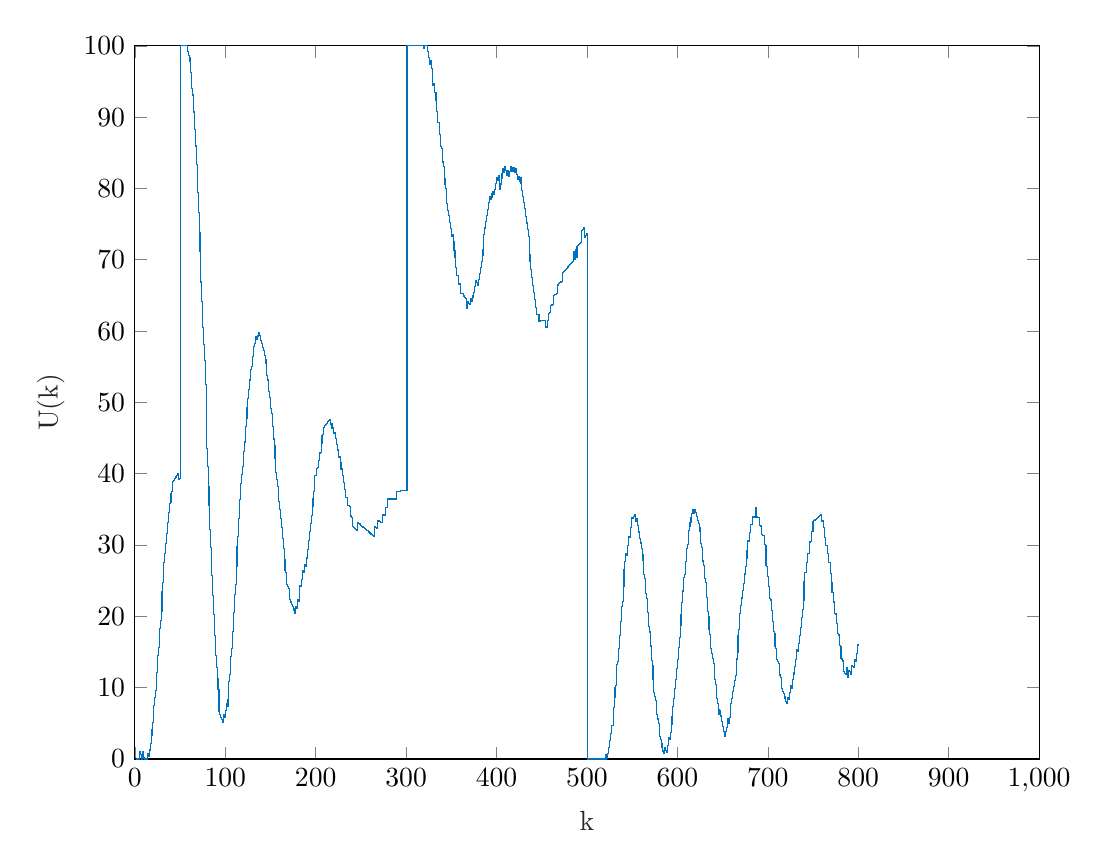
\begin{tikzpicture}

\begin{axis}[%
width=4.521in,
height=3.566in,
at={(0.758in,0.481in)},
scale only axis,
xmin=0,
xmax=1000,
xlabel style={font=\color{white!15!black}},
xlabel={k},
ymin=0,
ymax=100,
ylabel style={font=\color{white!15!black}},
ylabel={U(k)},
axis background/.style={fill=white}
]
\addplot[const plot, color=mycolor1, forget plot] table[row sep=crcr] {%
1	0\\
2	0\\
3	0\\
4	0\\
5	1.02025\\
6	0.58275\\
7	0\\
8	1.02025\\
9	0.58275\\
10	0.14525\\
11	0\\
12	0\\
13	0\\
14	0.833\\
15	0.4165\\
16	1.2705\\
17	2.1455\\
18	3.25325\\
19	4.17375\\
20	5.11525\\
21	7.56\\
22	8.568\\
23	9.597\\
24	12.12925\\
25	14.49525\\
26	15.63275\\
27	18.2735\\
28	19.4775\\
29	20.7025\\
30	23.43075\\
31	24.72225\\
32	27.517\\
33	28.875\\
34	30.254\\
35	31.644348\\
36	33.204212\\
37	34.525869\\
38	35.816087\\
39	36.015057\\
40	37.266466\\
41	37.47976\\
42	38.85912\\
43	39.088398\\
44	39.316817\\
45	39.544379\\
46	39.771087\\
47	39.996946\\
48	39.161328\\
49	39.36818\\
50	100\\
51	100\\
52	100\\
53	100\\
54	100\\
55	100\\
56	100\\
57	100\\
58	99.249727\\
59	98.661727\\
60	97.816\\
61	98.404\\
62	96.214273\\
63	93.952\\
64	93.100545\\
65	90.719909\\
66	88.266727\\
67	85.952909\\
68	83.358455\\
69	79.42\\
70	76.657545\\
71	73.822545\\
72	71.126909\\
73	66.879182\\
74	64.101819\\
75	60.465375\\
76	58.159304\\
77	55.841804\\
78	52.558304\\
79	43.594304\\
80	40.958804\\
81	38.266304\\
82	35.484013\\
83	32.16919\\
84	29.606691\\
85	25.770691\\
86	22.930441\\
87	20.256441\\
88	17.328691\\
89	14.567191\\
90	12.822441\\
91	11.264941\\
92	9.686441\\
93	6.604691\\
94	6.230191\\
95	5.855691\\
96	5.481191\\
97	5.106691\\
98	6.214441\\
99	5.864441\\
100	6.784941\\
101	7.726441\\
102	7.418441\\
103	8.380941\\
104	10.846691\\
105	11.875691\\
106	14.407941\\
107	15.503441\\
108	17.890441\\
109	20.531191\\
110	23.005691\\
111	24.463441\\
112	27.004441\\
113	29.799191\\
114	31.157191\\
115	33.721232\\
116	36.325016\\
117	38.587007\\
118	39.915905\\
119	41.05326\\
120	43.11426\\
121	44.45376\\
122	46.57176\\
123	47.81676\\
124	49.23126\\
125	50.51526\\
126	51.81726\\
127	53.13726\\
128	54.62676\\
129	55.07676\\
130	56.43576\\
131	57.81276\\
132	58.29876\\
133	58.78476\\
134	59.27076\\
135	58.84776\\
136	59.31576\\
137	59.78376\\
138	59.34276\\
139	58.73226\\
140	58.25226\\
141	57.75426\\
142	57.23826\\
143	56.55276\\
144	55.99776\\
145	55.42476\\
146	53.77326\\
147	53.14326\\
148	51.58626\\
149	50.75076\\
150	49.13676\\
151	48.39576\\
152	46.57626\\
153	44.86926\\
154	43.88376\\
155	42.11976\\
156	40.16826\\
157	39.23826\\
158	38.262228\\
159	36.097966\\
160	34.945664\\
161	33.730347\\
162	32.448906\\
163	30.90106\\
164	29.466202\\
165	27.975202\\
166	26.463202\\
167	26.200702\\
168	24.455952\\
169	24.168952\\
170	23.881952\\
171	22.324452\\
172	22.016452\\
173	21.708452\\
174	21.400452\\
175	21.092452\\
176	20.784452\\
177	20.476452\\
178	21.438952\\
179	21.151952\\
180	22.347202\\
181	22.084702\\
182	24.363202\\
183	24.142702\\
184	25.192702\\
185	26.475452\\
186	26.300452\\
187	26.125452\\
188	27.220952\\
189	27.066952\\
190	28.183452\\
191	29.320952\\
192	30.691202\\
193	31.850079\\
194	32.988956\\
195	34.107848\\
196	35.393787\\
197	36.469302\\
198	37.524996\\
199	39.725836\\
200	39.801178\\
201	40.792614\\
202	40.885614\\
203	41.887614\\
204	42.907614\\
205	43.036614\\
206	44.226114\\
207	45.285114\\
208	45.453114\\
209	46.530114\\
210	46.716114\\
211	46.902114\\
212	47.088114\\
213	47.274114\\
214	47.460114\\
215	47.646114\\
216	46.923114\\
217	47.091114\\
218	46.350114\\
219	46.500114\\
220	45.589614\\
221	45.718614\\
222	44.938614\\
223	44.140614\\
224	43.324614\\
225	42.339114\\
226	42.393114\\
227	41.538114\\
228	40.665114\\
229	40.683114\\
230	39.792114\\
231	38.722847\\
232	37.746231\\
233	36.715292\\
234	36.655171\\
235	35.565078\\
236	35.484535\\
237	35.40389\\
238	34.068804\\
239	33.963314\\
240	33.857656\\
241	32.620782\\
242	32.492762\\
243	32.364498\\
244	32.23599\\
245	32.107239\\
246	33.172566\\
247	33.065642\\
248	32.958547\\
249	32.851281\\
250	32.743843\\
251	32.636233\\
252	32.528451\\
253	32.420496\\
254	32.312369\\
255	32.204069\\
256	32.095595\\
257	31.986948\\
258	31.878128\\
259	31.769133\\
260	31.659963\\
261	31.550619\\
262	31.4411\\
263	31.331406\\
264	31.221536\\
265	32.542222\\
266	32.4579\\
267	32.373472\\
268	33.473638\\
269	33.410438\\
270	33.347178\\
271	33.283858\\
272	33.220478\\
273	33.157037\\
274	34.249909\\
275	34.207172\\
276	34.164406\\
277	35.24157\\
278	35.218905\\
279	36.458374\\
280	36.458374\\
281	36.458374\\
282	36.458374\\
283	36.458374\\
284	36.458374\\
285	36.458374\\
286	36.458374\\
287	36.458374\\
288	36.458374\\
289	37.495404\\
290	37.514155\\
291	37.532901\\
292	37.551641\\
293	37.570375\\
294	37.589104\\
295	37.607828\\
296	37.626545\\
297	37.645257\\
298	37.663964\\
299	37.682664\\
300	37.70136\\
301	100\\
302	100\\
303	100\\
304	100\\
305	100\\
306	100\\
307	100\\
308	100\\
309	100\\
310	100\\
311	100\\
312	100\\
313	100\\
314	100\\
315	100\\
316	100\\
317	100\\
318	100\\
319	99.690727\\
320	100\\
321	100\\
322	100\\
323	100\\
324	99.219182\\
325	98.365818\\
326	97.439909\\
327	97.924818\\
328	96.880545\\
329	94.492273\\
330	94.763364\\
331	93.505273\\
332	93.446091\\
333	92.277727\\
334	90.828727\\
335	89.307182\\
336	89.196455\\
337	87.556545\\
338	85.844091\\
339	85.542455\\
340	83.711636\\
341	83.079727\\
342	81.338636\\
343	80.588364\\
344	80.000364\\
345	77.883182\\
346	76.964909\\
347	76.208909\\
348	75.195182\\
349	74.343727\\
350	73.234545\\
351	73.559091\\
352	72.589273\\
353	71.361727\\
354	70.296455\\
355	68.973455\\
356	67.856738\\
357	67.738994\\
358	66.606171\\
359	66.629635\\
360	65.290785\\
361	65.261078\\
362	65.211106\\
363	64.958156\\
364	64.867306\\
365	64.757182\\
366	64.628127\\
367	63.224305\\
368	64.079422\\
369	63.89601\\
370	63.695401\\
371	64.520989\\
372	64.111787\\
373	64.922537\\
374	64.661986\\
375	65.463386\\
376	66.280326\\
377	67.113108\\
378	66.79522\\
379	66.461353\\
380	67.255301\\
381	68.063864\\
382	68.887313\\
383	69.72592\\
384	70.579966\\
385	71.439057\\
386	73.569602\\
387	74.451602\\
388	75.333602\\
389	76.215602\\
390	77.097602\\
391	77.979602\\
392	78.861602\\
393	78.472147\\
394	79.331238\\
395	78.706966\\
396	79.539329\\
397	79.100238\\
398	79.909693\\
399	80.719147\\
400	81.528602\\
401	81.066602\\
402	81.853147\\
403	79.884875\\
404	80.621784\\
405	81.358693\\
406	82.095602\\
407	82.832511\\
408	82.297966\\
409	83.011966\\
410	82.454511\\
411	81.874147\\
412	82.542329\\
413	81.727147\\
414	82.368602\\
415	83.010057\\
416	82.380057\\
417	82.998602\\
418	82.345693\\
419	82.941329\\
420	82.265511\\
421	82.838238\\
422	81.927602\\
423	81.202147\\
424	81.725238\\
425	80.976875\\
426	81.477057\\
427	80.705784\\
428	79.699693\\
429	78.878784\\
430	78.034966\\
431	77.168238\\
432	76.066693\\
433	75.150329\\
434	74.211057\\
435	73.248875\\
436	70.78042\\
437	69.745693\\
438	68.696109\\
439	67.453457\\
440	66.429526\\
441	65.417949\\
442	64.419314\\
443	63.255977\\
444	62.287758\\
445	62.326004\\
446	62.364288\\
447	61.407914\\
448	61.426606\\
449	61.445306\\
450	61.464015\\
451	61.482734\\
452	61.501462\\
453	61.520199\\
454	60.574845\\
455	60.574845\\
456	61.504681\\
457	62.486957\\
458	62.525399\\
459	62.563878\\
460	63.604325\\
461	63.663633\\
462	63.723028\\
463	65.000445\\
464	65.085673\\
465	65.171075\\
466	65.256652\\
467	66.441934\\
468	66.551274\\
469	66.66089\\
470	66.770784\\
471	66.880958\\
472	66.99141\\
473	68.26455\\
474	68.400569\\
475	68.537\\
476	68.673843\\
477	68.811102\\
478	68.948775\\
479	69.086866\\
480	69.225374\\
481	69.364302\\
482	69.50365\\
483	69.64342\\
484	69.783613\\
485	71.187843\\
486	70.08057\\
487	71.493297\\
488	70.386024\\
489	71.798752\\
490	71.962933\\
491	72.127115\\
492	72.291297\\
493	72.455479\\
494	74.103024\\
495	74.293933\\
496	74.484843\\
497	73.192388\\
498	73.35657\\
499	73.520752\\
500	73.684933\\
501	0\\
502	0\\
503	0\\
504	0\\
505	0\\
506	0\\
507	0\\
508	0\\
509	0\\
510	0\\
511	0\\
512	0\\
513	0\\
514	0\\
515	0\\
516	0\\
517	0\\
518	0\\
519	0\\
520	0\\
521	0.61075\\
522	0.0385\\
523	0.80325\\
524	1.6555\\
525	2.59525\\
526	3.6225\\
527	4.73725\\
528	4.669\\
529	7.20825\\
530	8.5855\\
531	10.05025\\
532	10.332\\
533	13.22125\\
534	13.678\\
535	15.47175\\
536	17.353\\
537	19.32175\\
538	21.378\\
539	22.0395\\
540	24.24625\\
541	26.5405\\
542	27.65175\\
543	28.8295\\
544	28.5915\\
545	29.87775\\
546	31.2305\\
547	31.124309\\
548	32.498004\\
549	33.828849\\
550	33.796884\\
551	33.994717\\
552	34.039022\\
553	34.308598\\
554	33.308079\\
555	33.674251\\
556	32.739247\\
557	31.829003\\
558	30.943944\\
559	30.290531\\
560	29.459245\\
561	28.650745\\
562	27.863245\\
563	25.826245\\
564	25.271495\\
565	23.258995\\
566	22.516995\\
567	20.525495\\
568	18.533995\\
569	17.812995\\
570	15.842495\\
571	13.871995\\
572	13.171995\\
573	11.222495\\
574	9.272995\\
575	8.805745\\
576	8.151245\\
577	6.247245\\
578	5.613745\\
579	5.001245\\
580	3.139245\\
581	2.759495\\
582	2.192495\\
583	1.646495\\
584	1.121495\\
585	0.829245\\
586	1.620245\\
587	1.182745\\
588	0.977995\\
589	1.856495\\
590	2.988745\\
591	2.684245\\
592	3.671245\\
593	4.911995\\
594	5.986495\\
595	7.314745\\
596	8.476745\\
597	9.892495\\
598	11.141995\\
599	12.645245\\
600	13.982245\\
601	15.572995\\
602	16.997495\\
603	18.675745\\
604	20.187745\\
605	21.953495\\
606	23.552995\\
607	25.406245\\
608	25.822745\\
609	27.742495\\
610	29.495995\\
611	30.020995\\
612	32.047818\\
613	32.585153\\
614	33.1285\\
615	33.870275\\
616	34.422229\\
617	34.978734\\
618	34.44881\\
619	35.024244\\
620	34.514184\\
621	34.00012\\
622	33.482021\\
623	32.959855\\
624	32.43359\\
625	31.903194\\
626	30.166934\\
627	29.597795\\
628	27.756795\\
629	27.165295\\
630	25.303295\\
631	24.690795\\
632	22.596045\\
633	20.688545\\
634	20.030545\\
635	18.102045\\
636	17.423045\\
637	15.473545\\
638	14.773545\\
639	14.073545\\
640	13.373545\\
641	11.191295\\
642	10.466795\\
643	8.471795\\
644	7.726295\\
645	6.980795\\
646	6.235295\\
647	6.760295\\
648	6.035795\\
649	5.311295\\
650	4.586795\\
651	3.862295\\
652	3.137795\\
653	3.895545\\
654	4.466045\\
655	5.057545\\
656	5.670045\\
657	5.033045\\
658	5.878295\\
659	7.806795\\
660	8.506795\\
661	9.439545\\
662	10.185045\\
663	10.951545\\
664	11.739045\\
665	14.029795\\
666	14.883795\\
667	17.241045\\
668	18.161545\\
669	20.373545\\
670	21.568795\\
671	22.576795\\
672	23.605795\\
673	24.655795\\
674	25.938545\\
675	27.034045\\
676	28.150545\\
677	29.288045\\
678	30.658295\\
679	30.571617\\
680	31.734668\\
681	32.877608\\
682	32.833978\\
683	33.958372\\
684	33.935257\\
685	33.912135\\
686	35.20626\\
687	33.943584\\
688	33.920464\\
689	33.897336\\
690	33.8742\\
691	32.720608\\
692	32.676877\\
693	31.459386\\
694	31.394272\\
695	31.329097\\
696	30.041406\\
697	29.953958\\
698	27.113708\\
699	26.980708\\
700	25.577208\\
701	24.152708\\
702	22.495458\\
703	22.295958\\
704	20.825958\\
705	19.334958\\
706	17.822958\\
707	17.560458\\
708	15.815708\\
709	15.528708\\
710	13.971208\\
711	13.663208\\
712	13.355208\\
713	11.776708\\
714	11.447708\\
715	9.848208\\
716	9.498208\\
717	9.148208\\
718	8.798208\\
719	8.448208\\
720	8.098208\\
721	7.748208\\
722	8.668708\\
723	8.339708\\
724	9.281208\\
725	10.243708\\
726	9.956708\\
727	11.151958\\
728	12.159958\\
729	11.918458\\
730	12.947458\\
731	13.997458\\
732	15.280208\\
733	15.105208\\
734	16.200708\\
735	17.317208\\
736	18.454708\\
737	19.824958\\
738	21.007958\\
739	22.211958\\
740	24.919208\\
741	26.189708\\
742	26.210708\\
743	27.502208\\
744	28.814708\\
745	28.877708\\
746	30.422958\\
747	30.509929\\
748	31.848858\\
749	31.954492\\
750	33.259808\\
751	33.383277\\
752	33.506518\\
753	33.629531\\
754	33.752317\\
755	33.874875\\
756	33.997206\\
757	34.119311\\
758	34.241191\\
759	33.245664\\
760	33.349133\\
761	33.452442\\
762	32.409896\\
763	31.113771\\
764	29.945532\\
765	29.987532\\
766	28.759032\\
767	27.509532\\
768	27.509532\\
769	26.027282\\
770	24.732282\\
771	23.416282\\
772	23.349782\\
773	22.012782\\
774	20.443032\\
775	20.331032\\
776	18.948532\\
777	17.545032\\
778	17.391032\\
779	15.966532\\
780	15.791532\\
781	14.134282\\
782	13.934782\\
783	13.735282\\
784	12.265282\\
785	12.044782\\
786	11.824282\\
787	12.874282\\
788	11.404282\\
789	12.454282\\
790	12.254782\\
791	12.055282\\
792	11.855782\\
793	13.138532\\
794	12.963532\\
795	12.788532\\
796	13.884032\\
797	13.730032\\
798	14.846532\\
799	15.984032\\
800	15.872032\\
};
\end{axis}
\end{tikzpicture}%
\caption{Sterowanie dla rozmytego PID}
\end{figure}

Wartość wskaźnika jakości:

\begin{equation}
E =23,2405e+07
\end{equation}

Osiągnięte wartości wskażnika jakośći regulacji są gorsze od regulatora klasycznego. W przypadku regulacji rozmytej z regulatorem PID największym utrudnieniem jest 
dobór nastaw dla każdego z regulatorów lokalnych. W przypadku stanowiska grzejąco-chłodzącego zadanie to jest bardzo czasochłonne tak aby uzyskać dostatecznie zadowalającą jakość regulacji.

\section{Rozmyty algorytm DMC}

Dla tej samej trajektorii zmian sygnału wartości zadanej, został zastosowany rozmyty algorytm DMC w najprostszej wersji analitycznej dla trzech regulatorów lokalnych. Dla każdego z regulatorów metodą inżynierską starano się 
dobrać odpowiednie nastawy w taki sposób aby uzyskać lepszą jakość regulacji w porównaniu z regulatorem klasycznym.


Wyniki działania regulacji dla następujących nastaw regulatorów lokalnych:

Regulator DMC 1
\begin{equation}
N = 20; 
N_u = 20; 
\lambda = 1; 
\end{equation}

Regulator DMC 2
\begin{equation}
N = 20; 
N_u = 20; 
\lambda = 1; 
\end{equation}

Regulator DMC 3
\begin{equation}
N = 20; 
N_u = 20; 
\lambda =1; 
\end{equation}

\begin{figure}[H]
\centering
% This file was created by matlab2tikz.
%
%The latest updates can be retrieved from
%  http://www.mathworks.com/matlabcentral/fileexchange/22022-matlab2tikz-matlab2tikz
%where you can also make suggestions and rate matlab2tikz.
%
\definecolor{mycolor1}{rgb}{0.00000,0.44700,0.74100}%
%
\begin{tikzpicture}

\begin{axis}[%
width=4.521in,
height=3.566in,
at={(0.758in,0.481in)},
scale only axis,
xmin=0,
xmax=1000,
xlabel style={font=\color{white!15!black}},
xlabel={k},
ymin=26,
ymax=46,
ylabel style={font=\color{white!15!black}},
ylabel={Y(k)},
axis background/.style={fill=white}
]
\addplot[const plot, color=mycolor1, forget plot] table[row sep=crcr] {%
1	30.5\\
2	30.43\\
3	30.43\\
4	30.43\\
5	30.43\\
6	30.43\\
7	30.5\\
8	30.5\\
9	30.5\\
10	30.5\\
11	30.5\\
12	30.5\\
13	30.5\\
14	30.5\\
15	30.5\\
16	30.5\\
17	30.56\\
18	30.56\\
19	30.56\\
20	30.56\\
21	30.56\\
22	30.62\\
23	30.62\\
24	30.62\\
25	30.62\\
26	30.56\\
27	30.56\\
28	30.5\\
29	30.5\\
30	30.43\\
31	30.37\\
32	30.31\\
33	30.18\\
34	30.12\\
35	30.06\\
36	30\\
37	29.93\\
38	29.81\\
39	29.75\\
40	29.62\\
41	29.5\\
42	29.37\\
43	29.31\\
44	29.25\\
45	29.12\\
46	29.06\\
47	28.93\\
48	28.81\\
49	28.75\\
50	28.68\\
51	28.62\\
52	28.5\\
53	28.43\\
54	28.37\\
55	28.31\\
56	28.18\\
57	28.12\\
58	28.06\\
59	28.06\\
60	28\\
61	27.93\\
62	27.87\\
63	27.87\\
64	27.87\\
65	27.87\\
66	27.87\\
67	27.93\\
68	27.93\\
69	28\\
70	28.06\\
71	28.12\\
72	28.18\\
73	28.18\\
74	28.31\\
75	28.37\\
76	28.43\\
77	28.56\\
78	28.62\\
79	28.68\\
80	28.81\\
81	28.87\\
82	29\\
83	29.06\\
84	29.18\\
85	29.31\\
86	29.37\\
87	29.5\\
88	29.56\\
89	29.68\\
90	29.81\\
91	29.87\\
92	29.93\\
93	30\\
94	30.06\\
95	30.12\\
96	30.18\\
97	30.25\\
98	30.31\\
99	30.37\\
100	30.43\\
101	30.43\\
102	30.5\\
103	30.5\\
104	30.56\\
105	30.56\\
106	30.62\\
107	30.62\\
108	30.62\\
109	30.62\\
110	30.62\\
111	30.62\\
112	30.62\\
113	30.62\\
114	30.62\\
115	30.62\\
116	30.62\\
117	30.62\\
118	30.62\\
119	30.62\\
120	30.62\\
121	30.62\\
122	30.62\\
123	30.62\\
124	30.56\\
125	30.56\\
126	30.56\\
127	30.56\\
128	30.56\\
129	30.56\\
130	30.56\\
131	30.56\\
132	30.56\\
133	30.56\\
134	30.56\\
135	30.56\\
136	30.56\\
137	30.5\\
138	30.5\\
139	30.56\\
140	30.56\\
141	30.56\\
142	30.56\\
143	30.56\\
144	30.56\\
145	30.56\\
146	30.56\\
147	30.56\\
148	30.56\\
149	30.5\\
150	30.5\\
151	30.5\\
152	30.5\\
153	30.56\\
154	30.5\\
155	30.56\\
156	30.56\\
157	30.56\\
158	30.56\\
159	30.56\\
160	30.56\\
161	30.56\\
162	30.56\\
163	30.56\\
164	30.56\\
165	30.56\\
166	30.56\\
167	30.56\\
168	30.56\\
169	30.62\\
170	30.56\\
171	30.56\\
172	30.56\\
173	30.56\\
174	30.56\\
175	30.56\\
176	30.56\\
177	30.56\\
178	30.56\\
179	30.56\\
180	30.56\\
181	30.56\\
182	30.56\\
183	30.56\\
184	30.62\\
185	30.62\\
186	30.62\\
187	30.62\\
188	30.62\\
189	30.62\\
190	30.62\\
191	30.62\\
192	30.62\\
193	30.62\\
194	30.62\\
195	30.56\\
196	30.62\\
197	30.62\\
198	30.56\\
199	30.62\\
200	30.62\\
201	30.56\\
202	30.62\\
203	30.56\\
204	30.56\\
205	30.56\\
206	30.56\\
207	30.5\\
208	30.5\\
209	30.5\\
210	30.5\\
211	30.5\\
212	30.5\\
213	30.5\\
214	30.56\\
215	30.5\\
216	30.5\\
217	30.56\\
218	30.5\\
219	30.5\\
220	30.56\\
221	30.56\\
222	30.56\\
223	30.5\\
224	30.56\\
225	30.5\\
226	30.5\\
227	30.5\\
228	30.56\\
229	30.5\\
230	30.5\\
231	30.5\\
232	30.56\\
233	30.5\\
234	30.5\\
235	30.5\\
236	30.5\\
237	30.5\\
238	30.5\\
239	30.5\\
240	30.5\\
241	30.5\\
242	30.5\\
243	30.5\\
244	30.56\\
245	30.56\\
246	30.56\\
247	30.56\\
248	30.62\\
249	30.62\\
250	30.62\\
251	30.62\\
252	30.62\\
253	30.62\\
254	30.62\\
255	30.62\\
256	30.62\\
257	30.62\\
258	30.62\\
259	30.62\\
260	30.62\\
261	30.62\\
262	30.62\\
263	30.62\\
264	30.62\\
265	30.62\\
266	30.62\\
267	30.62\\
268	30.62\\
269	30.62\\
270	30.62\\
271	30.62\\
272	30.62\\
273	30.62\\
274	30.62\\
275	30.62\\
276	30.62\\
277	30.62\\
278	30.62\\
279	30.56\\
280	30.62\\
281	30.56\\
282	30.56\\
283	30.62\\
284	30.56\\
285	30.62\\
286	30.56\\
287	30.62\\
288	30.62\\
289	30.62\\
290	30.62\\
291	30.62\\
292	30.62\\
293	30.56\\
294	30.56\\
295	30.62\\
296	30.62\\
297	30.62\\
298	30.62\\
299	30.62\\
300	30.62\\
301	30.62\\
302	30.62\\
303	30.62\\
304	30.68\\
305	30.62\\
306	30.68\\
307	30.62\\
308	30.62\\
309	30.62\\
310	30.68\\
311	30.68\\
312	30.68\\
313	30.68\\
314	30.75\\
315	30.75\\
316	30.81\\
317	30.87\\
318	30.93\\
319	31\\
320	31.06\\
321	31.18\\
322	31.25\\
323	31.37\\
324	31.5\\
325	31.56\\
326	31.68\\
327	31.81\\
328	31.93\\
329	32.06\\
330	32.25\\
331	32.37\\
332	32.56\\
333	32.68\\
334	32.81\\
335	32.93\\
336	33.12\\
337	33.25\\
338	33.43\\
339	33.56\\
340	33.75\\
341	33.93\\
342	34.06\\
343	34.18\\
344	34.31\\
345	34.43\\
346	34.56\\
347	34.68\\
348	34.81\\
349	34.93\\
350	35.06\\
351	35.12\\
352	35.25\\
353	35.37\\
354	35.5\\
355	35.56\\
356	35.68\\
357	35.75\\
358	35.87\\
359	35.93\\
360	36\\
361	36.06\\
362	36.12\\
363	36.18\\
364	36.25\\
365	36.31\\
366	36.37\\
367	36.37\\
368	36.43\\
369	36.5\\
370	36.5\\
371	36.56\\
372	36.56\\
373	36.62\\
374	36.62\\
375	36.68\\
376	36.68\\
377	36.68\\
378	36.75\\
379	36.75\\
380	36.75\\
381	36.75\\
382	36.75\\
383	36.75\\
384	36.75\\
385	36.68\\
386	36.68\\
387	36.68\\
388	36.62\\
389	36.62\\
390	36.62\\
391	36.62\\
392	36.62\\
393	36.62\\
394	36.62\\
395	36.56\\
396	36.62\\
397	36.56\\
398	36.56\\
399	36.56\\
400	36.5\\
401	36.5\\
402	36.5\\
403	36.5\\
404	36.5\\
405	36.43\\
406	36.43\\
407	36.43\\
408	36.43\\
409	36.43\\
410	36.37\\
411	36.37\\
412	36.37\\
413	36.37\\
414	36.37\\
415	36.31\\
416	36.31\\
417	36.31\\
418	36.31\\
419	36.25\\
420	36.25\\
421	36.25\\
422	36.25\\
423	36.25\\
424	36.25\\
425	36.25\\
426	36.31\\
427	36.31\\
428	36.31\\
429	36.31\\
430	36.31\\
431	36.31\\
432	36.31\\
433	36.37\\
434	36.37\\
};
\addplot [color=red, dashed, forget plot]
  table[row sep=crcr]{%
1	30.93\\
2	30.93\\
3	30.93\\
4	30.93\\
5	30.93\\
6	30.93\\
7	30.93\\
8	30.93\\
9	30.93\\
10	30.93\\
11	30.93\\
12	30.93\\
13	30.93\\
14	30.93\\
15	30.93\\
16	30.93\\
17	30.93\\
18	30.93\\
19	30.93\\
20	30.93\\
21	30.93\\
22	30.93\\
23	30.93\\
24	30.93\\
25	30.93\\
26	30.93\\
27	30.93\\
28	30.93\\
29	30.93\\
30	30.93\\
31	30.93\\
32	30.93\\
33	30.93\\
34	30.93\\
35	30.93\\
36	30.93\\
37	30.93\\
38	30.93\\
39	30.93\\
40	30.93\\
41	30.93\\
42	30.93\\
43	30.93\\
44	30.93\\
45	30.93\\
46	30.93\\
47	30.93\\
48	30.93\\
49	30.93\\
50	30.93\\
51	35.93\\
52	35.93\\
53	35.93\\
54	35.93\\
55	35.93\\
56	35.93\\
57	35.93\\
58	35.93\\
59	35.93\\
60	35.93\\
61	35.93\\
62	35.93\\
63	35.93\\
64	35.93\\
65	35.93\\
66	35.93\\
67	35.93\\
68	35.93\\
69	35.93\\
70	35.93\\
71	35.93\\
72	35.93\\
73	35.93\\
74	35.93\\
75	35.93\\
76	35.93\\
77	35.93\\
78	35.93\\
79	35.93\\
80	35.93\\
81	35.93\\
82	35.93\\
83	35.93\\
84	35.93\\
85	35.93\\
86	35.93\\
87	35.93\\
88	35.93\\
89	35.93\\
90	35.93\\
91	35.93\\
92	35.93\\
93	35.93\\
94	35.93\\
95	35.93\\
96	35.93\\
97	35.93\\
98	35.93\\
99	35.93\\
100	35.93\\
101	35.93\\
102	35.93\\
103	35.93\\
104	35.93\\
105	35.93\\
106	35.93\\
107	35.93\\
108	35.93\\
109	35.93\\
110	35.93\\
111	35.93\\
112	35.93\\
113	35.93\\
114	35.93\\
115	35.93\\
116	35.93\\
117	35.93\\
118	35.93\\
119	35.93\\
120	35.93\\
121	35.93\\
122	35.93\\
123	35.93\\
124	35.93\\
125	35.93\\
126	35.93\\
127	35.93\\
128	35.93\\
129	35.93\\
130	35.93\\
131	35.93\\
132	35.93\\
133	35.93\\
134	35.93\\
135	35.93\\
136	35.93\\
137	35.93\\
138	35.93\\
139	35.93\\
140	35.93\\
141	35.93\\
142	35.93\\
143	35.93\\
144	35.93\\
145	35.93\\
146	35.93\\
147	35.93\\
148	35.93\\
149	35.93\\
150	35.93\\
151	35.93\\
152	35.93\\
153	35.93\\
154	35.93\\
155	35.93\\
156	35.93\\
157	35.93\\
158	35.93\\
159	35.93\\
160	35.93\\
161	35.93\\
162	35.93\\
163	35.93\\
164	35.93\\
165	35.93\\
166	35.93\\
167	35.93\\
168	35.93\\
169	35.93\\
170	35.93\\
171	35.93\\
172	35.93\\
173	35.93\\
174	35.93\\
175	35.93\\
176	35.93\\
177	35.93\\
178	35.93\\
179	35.93\\
180	35.93\\
181	35.93\\
182	35.93\\
183	35.93\\
184	35.93\\
185	35.93\\
186	35.93\\
187	35.93\\
188	35.93\\
189	35.93\\
190	35.93\\
191	35.93\\
192	35.93\\
193	35.93\\
194	35.93\\
195	35.93\\
196	35.93\\
197	35.93\\
198	35.93\\
199	35.93\\
200	35.93\\
201	35.93\\
202	35.93\\
203	35.93\\
204	35.93\\
205	35.93\\
206	35.93\\
207	35.93\\
208	35.93\\
209	35.93\\
210	35.93\\
211	35.93\\
212	35.93\\
213	35.93\\
214	35.93\\
215	35.93\\
216	35.93\\
217	35.93\\
218	35.93\\
219	35.93\\
220	35.93\\
221	35.93\\
222	35.93\\
223	35.93\\
224	35.93\\
225	35.93\\
226	35.93\\
227	35.93\\
228	35.93\\
229	35.93\\
230	35.93\\
231	35.93\\
232	35.93\\
233	35.93\\
234	35.93\\
235	35.93\\
236	35.93\\
237	35.93\\
238	35.93\\
239	35.93\\
240	35.93\\
241	35.93\\
242	35.93\\
243	35.93\\
244	35.93\\
245	35.93\\
246	35.93\\
247	35.93\\
248	35.93\\
249	35.93\\
250	35.93\\
251	35.93\\
252	35.93\\
253	35.93\\
254	35.93\\
255	35.93\\
256	35.93\\
257	35.93\\
258	35.93\\
259	35.93\\
260	35.93\\
261	35.93\\
262	35.93\\
263	35.93\\
264	35.93\\
265	35.93\\
266	35.93\\
267	35.93\\
268	35.93\\
269	35.93\\
270	35.93\\
271	35.93\\
272	35.93\\
273	35.93\\
274	35.93\\
275	35.93\\
276	35.93\\
277	35.93\\
278	35.93\\
279	35.93\\
280	35.93\\
281	35.93\\
282	35.93\\
283	35.93\\
284	35.93\\
285	35.93\\
286	35.93\\
287	35.93\\
288	35.93\\
289	35.93\\
290	35.93\\
291	35.93\\
292	35.93\\
293	35.93\\
294	35.93\\
295	35.93\\
296	35.93\\
297	35.93\\
298	35.93\\
299	35.93\\
300	35.93\\
301	45.93\\
302	45.93\\
303	45.93\\
304	45.93\\
305	45.93\\
306	45.93\\
307	45.93\\
308	45.93\\
309	45.93\\
310	45.93\\
311	45.93\\
312	45.93\\
313	45.93\\
314	45.93\\
315	45.93\\
316	45.93\\
317	45.93\\
318	45.93\\
319	45.93\\
320	45.93\\
321	45.93\\
322	45.93\\
323	45.93\\
324	45.93\\
325	45.93\\
326	45.93\\
327	45.93\\
328	45.93\\
329	45.93\\
330	45.93\\
331	45.93\\
332	45.93\\
333	45.93\\
334	45.93\\
335	45.93\\
336	45.93\\
337	45.93\\
338	45.93\\
339	45.93\\
340	45.93\\
341	45.93\\
342	45.93\\
343	45.93\\
344	45.93\\
345	45.93\\
346	45.93\\
347	45.93\\
348	45.93\\
349	45.93\\
350	45.93\\
351	45.93\\
352	45.93\\
353	45.93\\
354	45.93\\
355	45.93\\
356	45.93\\
357	45.93\\
358	45.93\\
359	45.93\\
360	45.93\\
361	45.93\\
362	45.93\\
363	45.93\\
364	45.93\\
365	45.93\\
366	45.93\\
367	45.93\\
368	45.93\\
369	45.93\\
370	45.93\\
371	45.93\\
372	45.93\\
373	45.93\\
374	45.93\\
375	45.93\\
376	45.93\\
377	45.93\\
378	45.93\\
379	45.93\\
380	45.93\\
381	45.93\\
382	45.93\\
383	45.93\\
384	45.93\\
385	45.93\\
386	45.93\\
387	45.93\\
388	45.93\\
389	45.93\\
390	45.93\\
391	45.93\\
392	45.93\\
393	45.93\\
394	45.93\\
395	45.93\\
396	45.93\\
397	45.93\\
398	45.93\\
399	45.93\\
400	45.93\\
401	45.93\\
402	45.93\\
403	45.93\\
404	45.93\\
405	45.93\\
406	45.93\\
407	45.93\\
408	45.93\\
409	45.93\\
410	45.93\\
411	45.93\\
412	45.93\\
413	45.93\\
414	45.93\\
415	45.93\\
416	45.93\\
417	45.93\\
418	45.93\\
419	45.93\\
420	45.93\\
421	45.93\\
422	45.93\\
423	45.93\\
424	45.93\\
425	45.93\\
426	45.93\\
427	45.93\\
428	45.93\\
429	45.93\\
430	45.93\\
431	45.93\\
432	45.93\\
433	45.93\\
434	45.93\\
435	45.93\\
436	45.93\\
437	45.93\\
438	45.93\\
439	45.93\\
440	45.93\\
441	45.93\\
442	45.93\\
443	45.93\\
444	45.93\\
445	45.93\\
446	45.93\\
447	45.93\\
448	45.93\\
449	45.93\\
450	45.93\\
451	45.93\\
452	45.93\\
453	45.93\\
454	45.93\\
455	45.93\\
456	45.93\\
457	45.93\\
458	45.93\\
459	45.93\\
460	45.93\\
461	45.93\\
462	45.93\\
463	45.93\\
464	45.93\\
465	45.93\\
466	45.93\\
467	45.93\\
468	45.93\\
469	45.93\\
470	45.93\\
471	45.93\\
472	45.93\\
473	45.93\\
474	45.93\\
475	45.93\\
476	45.93\\
477	45.93\\
478	45.93\\
479	45.93\\
480	45.93\\
481	45.93\\
482	45.93\\
483	45.93\\
484	45.93\\
485	45.93\\
486	45.93\\
487	45.93\\
488	45.93\\
489	45.93\\
490	45.93\\
491	45.93\\
492	45.93\\
493	45.93\\
494	45.93\\
495	45.93\\
496	45.93\\
497	45.93\\
498	45.93\\
499	45.93\\
500	45.93\\
501	30.93\\
502	30.93\\
503	30.93\\
504	30.93\\
505	30.93\\
506	30.93\\
507	30.93\\
508	30.93\\
509	30.93\\
510	30.93\\
511	30.93\\
512	30.93\\
513	30.93\\
514	30.93\\
515	30.93\\
516	30.93\\
517	30.93\\
518	30.93\\
519	30.93\\
520	30.93\\
521	30.93\\
522	30.93\\
523	30.93\\
524	30.93\\
525	30.93\\
526	30.93\\
527	30.93\\
528	30.93\\
529	30.93\\
530	30.93\\
531	30.93\\
532	30.93\\
533	30.93\\
534	30.93\\
535	30.93\\
536	30.93\\
537	30.93\\
538	30.93\\
539	30.93\\
540	30.93\\
541	30.93\\
542	30.93\\
543	30.93\\
544	30.93\\
545	30.93\\
546	30.93\\
547	30.93\\
548	30.93\\
549	30.93\\
550	30.93\\
551	30.93\\
552	30.93\\
553	30.93\\
554	30.93\\
555	30.93\\
556	30.93\\
557	30.93\\
558	30.93\\
559	30.93\\
560	30.93\\
561	30.93\\
562	30.93\\
563	30.93\\
564	30.93\\
565	30.93\\
566	30.93\\
567	30.93\\
568	30.93\\
569	30.93\\
570	30.93\\
571	30.93\\
572	30.93\\
573	30.93\\
574	30.93\\
575	30.93\\
576	30.93\\
577	30.93\\
578	30.93\\
579	30.93\\
580	30.93\\
581	30.93\\
582	30.93\\
583	30.93\\
584	30.93\\
585	30.93\\
586	30.93\\
587	30.93\\
588	30.93\\
589	30.93\\
590	30.93\\
591	30.93\\
592	30.93\\
593	30.93\\
594	30.93\\
595	30.93\\
596	30.93\\
597	30.93\\
598	30.93\\
599	30.93\\
600	30.93\\
601	30.93\\
602	30.93\\
603	30.93\\
604	30.93\\
605	30.93\\
606	30.93\\
607	30.93\\
608	30.93\\
609	30.93\\
610	30.93\\
611	30.93\\
612	30.93\\
613	30.93\\
614	30.93\\
615	30.93\\
616	30.93\\
617	30.93\\
618	30.93\\
619	30.93\\
620	30.93\\
621	30.93\\
622	30.93\\
623	30.93\\
624	30.93\\
625	30.93\\
626	30.93\\
627	30.93\\
628	30.93\\
629	30.93\\
630	30.93\\
631	30.93\\
632	30.93\\
633	30.93\\
634	30.93\\
635	30.93\\
636	30.93\\
637	30.93\\
638	30.93\\
639	30.93\\
640	30.93\\
641	30.93\\
642	30.93\\
643	30.93\\
644	30.93\\
645	30.93\\
646	30.93\\
647	30.93\\
648	30.93\\
649	30.93\\
650	30.93\\
651	30.93\\
652	30.93\\
653	30.93\\
654	30.93\\
655	30.93\\
656	30.93\\
657	30.93\\
658	30.93\\
659	30.93\\
660	30.93\\
661	30.93\\
662	30.93\\
663	30.93\\
664	30.93\\
665	30.93\\
666	30.93\\
667	30.93\\
668	30.93\\
669	30.93\\
670	30.93\\
671	30.93\\
672	30.93\\
673	30.93\\
674	30.93\\
675	30.93\\
676	30.93\\
677	30.93\\
678	30.93\\
679	30.93\\
680	30.93\\
681	30.93\\
682	30.93\\
683	30.93\\
684	30.93\\
685	30.93\\
686	30.93\\
687	30.93\\
688	30.93\\
689	30.93\\
690	30.93\\
691	30.93\\
692	30.93\\
693	30.93\\
694	30.93\\
695	30.93\\
696	30.93\\
697	30.93\\
698	30.93\\
699	30.93\\
700	30.93\\
701	30.93\\
702	30.93\\
703	30.93\\
704	30.93\\
705	30.93\\
706	30.93\\
707	30.93\\
708	30.93\\
709	30.93\\
710	30.93\\
711	30.93\\
712	30.93\\
713	30.93\\
714	30.93\\
715	30.93\\
716	30.93\\
717	30.93\\
718	30.93\\
719	30.93\\
720	30.93\\
721	30.93\\
722	30.93\\
723	30.93\\
724	30.93\\
725	30.93\\
726	30.93\\
727	30.93\\
728	30.93\\
729	30.93\\
730	30.93\\
731	30.93\\
732	30.93\\
733	30.93\\
734	30.93\\
735	30.93\\
736	30.93\\
737	30.93\\
738	30.93\\
739	30.93\\
740	30.93\\
741	30.93\\
742	30.93\\
743	30.93\\
744	30.93\\
745	30.93\\
746	30.93\\
747	30.93\\
748	30.93\\
749	30.93\\
750	30.93\\
751	30.93\\
752	30.93\\
753	30.93\\
754	30.93\\
755	30.93\\
756	30.93\\
757	30.93\\
758	30.93\\
759	30.93\\
760	30.93\\
761	30.93\\
762	30.93\\
763	30.93\\
764	30.93\\
765	30.93\\
766	30.93\\
767	30.93\\
768	30.93\\
769	30.93\\
770	30.93\\
771	30.93\\
772	30.93\\
773	30.93\\
774	30.93\\
775	30.93\\
776	30.93\\
777	30.93\\
778	30.93\\
779	30.93\\
780	30.93\\
781	30.93\\
782	30.93\\
783	30.93\\
784	30.93\\
785	30.93\\
786	30.93\\
787	30.93\\
788	30.93\\
789	30.93\\
790	30.93\\
791	30.93\\
792	30.93\\
793	30.93\\
794	30.93\\
795	30.93\\
796	30.93\\
797	30.93\\
798	30.93\\
799	30.93\\
800	30.93\\
};
\end{axis}
\end{tikzpicture}%
\caption{Regulacja dla rozmytego DMC}
\end{figure}

\begin{figure}[H]
\centering
% This file was created by matlab2tikz.
%
%The latest updates can be retrieved from
%  http://www.mathworks.com/matlabcentral/fileexchange/22022-matlab2tikz-matlab2tikz
%where you can also make suggestions and rate matlab2tikz.
%
\definecolor{mycolor1}{rgb}{0.00000,0.44700,0.74100}%
%
\begin{tikzpicture}

\begin{axis}[%
width=4.521in,
height=3.566in,
at={(0.758in,0.481in)},
scale only axis,
xmin=0,
xmax=1000,
xlabel style={font=\color{white!15!black}},
xlabel={k},
ymin=0,
ymax=70,
ylabel style={font=\color{white!15!black}},
ylabel={U(k)},
axis background/.style={fill=white}
]
\addplot[const plot, color=mycolor1, forget plot] table[row sep=crcr] {%
1	31.218198\\
2	31.293714\\
3	31.176009\\
4	30.845339\\
5	30.340911\\
6	29.645055\\
7	28.708436\\
8	27.566568\\
9	26.211878\\
10	24.638136\\
11	22.840961\\
12	20.818004\\
13	18.568565\\
14	16.162591\\
15	13.67488\\
16	11.115306\\
17	8.462063\\
18	5.838354\\
19	3.327384\\
20	0.945099\\
21	0\\
22	0\\
23	0\\
24	0\\
25	0\\
26	0\\
27	0\\
28	0\\
29	0\\
30	0\\
31	0\\
32	0.092573\\
33	0.353326\\
34	0.720335\\
35	1.17014\\
36	1.683048\\
37	2.24606\\
38	2.867273\\
39	3.499796\\
40	4.170925\\
41	4.867473\\
42	5.589456\\
43	6.296166\\
44	6.983877\\
45	7.685762\\
46	8.360656\\
47	9.041878\\
48	9.720483\\
49	10.360979\\
50	13.617442\\
51	16.814714\\
52	19.965753\\
53	23.02431\\
54	25.970696\\
55	28.790385\\
56	31.505827\\
57	33.890962\\
58	35.853896\\
59	37.433369\\
60	38.71044\\
61	39.731656\\
62	40.529696\\
63	41.154393\\
64	41.626599\\
65	41.947698\\
66	42.121771\\
67	42.137501\\
68	42.021666\\
69	41.764432\\
70	41.38323\\
71	40.893833\\
72	40.31195\\
73	39.671114\\
74	38.942424\\
75	38.152977\\
76	37.312886\\
77	36.407325\\
78	35.470621\\
79	34.513716\\
80	33.517869\\
81	32.522232\\
82	31.505331\\
83	30.509761\\
84	29.51593\\
85	28.534852\\
86	27.618463\\
87	26.734104\\
88	25.922344\\
89	25.153612\\
90	24.42402\\
91	23.771214\\
92	23.194829\\
93	22.688357\\
94	22.254837\\
95	21.891238\\
96	21.593856\\
97	21.352886\\
98	21.168511\\
99	21.035103\\
100	20.946582\\
101	20.928436\\
102	20.936692\\
103	21.001529\\
104	21.083958\\
105	21.208845\\
106	21.337514\\
107	21.495209\\
108	21.675595\\
109	21.872695\\
110	22.080808\\
111	22.294671\\
112	22.509495\\
113	22.720951\\
114	22.925231\\
115	23.119022\\
116	23.299495\\
117	23.464276\\
118	23.611496\\
119	23.739733\\
120	23.847976\\
121	23.935712\\
122	24.002811\\
123	24.049542\\
124	24.108277\\
125	24.147928\\
126	24.169452\\
127	24.174051\\
128	24.163192\\
129	24.138493\\
130	24.101672\\
131	24.054508\\
132	23.998799\\
133	23.936322\\
134	23.8688\\
135	23.797876\\
136	23.725079\\
137	23.683701\\
138	23.643124\\
139	23.57255\\
140	23.504824\\
141	23.440945\\
142	23.381811\\
143	23.32808\\
144	23.280306\\
145	23.238877\\
146	23.204024\\
147	23.175828\\
148	23.154234\\
149	23.170883\\
150	23.193545\\
151	23.221767\\
152	23.254931\\
153	23.260512\\
154	23.301661\\
155	23.314091\\
156	23.329058\\
157	23.345925\\
158	23.364133\\
159	23.383007\\
160	23.401896\\
161	23.420192\\
162	23.437401\\
163	23.453154\\
164	23.467148\\
165	23.479143\\
166	23.488981\\
167	23.496641\\
168	23.502169\\
169	23.473856\\
170	23.475626\\
171	23.475831\\
172	23.474684\\
173	23.472224\\
174	23.468655\\
175	23.464141\\
176	23.458858\\
177	23.452996\\
178	23.446749\\
179	23.440311\\
180	23.433868\\
181	23.427597\\
182	23.42159\\
183	23.415924\\
184	23.378898\\
185	23.342629\\
186	23.307329\\
187	23.273219\\
188	23.240515\\
189	23.209358\\
190	23.17995\\
191	23.152488\\
192	23.127163\\
193	23.104159\\
194	23.083653\\
195	23.097637\\
196	23.082443\\
197	23.069957\\
198	23.091991\\
199	23.084758\\
200	23.080034\\
201	23.109504\\
202	23.109192\\
203	23.142503\\
204	23.177113\\
205	23.212569\\
206	23.248333\\
207	23.315747\\
208	23.382388\\
209	23.447639\\
210	23.510805\\
211	23.571324\\
212	23.628724\\
213	23.682467\\
214	23.700207\\
215	23.745429\\
216	23.785931\\
217	23.78954\\
218	23.81985\\
219	23.844842\\
220	23.832612\\
221	23.815263\\
222	23.793133\\
223	23.798504\\
224	23.768058\\
225	23.766048\\
226	23.761104\\
227	23.753758\\
228	23.712645\\
229	23.702193\\
230	23.691109\\
231	23.679819\\
232	23.636903\\
233	23.626627\\
234	23.61736\\
235	23.609316\\
236	23.602727\\
237	23.597685\\
238	23.594225\\
239	23.592391\\
240	23.592187\\
241	23.593486\\
242	23.59612\\
243	23.600089\\
244	23.573466\\
245	23.548048\\
246	23.523808\\
247	23.500861\\
248	23.44736\\
249	23.395284\\
250	23.344826\\
251	23.296274\\
252	23.249808\\
253	23.205699\\
254	23.164244\\
255	23.125765\\
256	23.090601\\
257	23.059043\\
258	23.031322\\
259	23.007678\\
260	22.988355\\
261	22.973448\\
262	22.962903\\
263	22.956657\\
264	22.954565\\
265	22.956386\\
266	22.961794\\
267	22.970448\\
268	22.981928\\
269	22.995801\\
270	23.011634\\
271	23.02899\\
272	23.047443\\
273	23.066575\\
274	23.085988\\
275	23.105305\\
276	23.124177\\
277	23.142289\\
278	23.159361\\
279	23.206973\\
280	23.221091\\
281	23.265183\\
282	23.307103\\
283	23.314799\\
284	23.35183\\
285	23.354393\\
286	23.386182\\
287	23.383387\\
288	23.377937\\
289	23.369906\\
290	23.359464\\
291	23.346741\\
292	23.331958\\
293	23.347179\\
294	23.36065\\
295	23.340675\\
296	23.319399\\
297	23.297205\\
298	23.274499\\
299	23.251755\\
300	23.229296\\
301	28.511294\\
302	33.763069\\
303	38.054434\\
304	41.242193\\
305	43.927642\\
306	46.511079\\
307	49.016243\\
308	51.412182\\
309	53.685452\\
310	55.804046\\
311	57.773548\\
312	59.582893\\
313	61.22291\\
314	62.660924\\
315	63.920492\\
316	64.990699\\
317	65.88078\\
318	66.601815\\
319	67.162562\\
320	67.578139\\
321	67.846434\\
322	67.994486\\
323	68.020173\\
324	67.92944\\
325	67.747952\\
326	67.466077\\
327	67.08674\\
328	66.617827\\
329	66.061551\\
330	65.405871\\
331	64.673831\\
332	63.850054\\
333	62.957664\\
334	61.998059\\
335	60.978311\\
336	59.882027\\
337	58.735435\\
338	57.571955\\
339	56.413004\\
340	55.246342\\
341	54.080348\\
342	52.934964\\
343	51.817558\\
344	50.728974\\
345	49.675557\\
346	48.65707\\
347	47.678751\\
348	46.739242\\
349	45.842655\\
350	44.986524\\
351	44.191935\\
352	43.437272\\
353	42.724526\\
354	42.049223\\
355	41.43059\\
356	40.848326\\
357	40.314952\\
358	39.812635\\
359	39.360152\\
360	38.957791\\
361	38.606032\\
362	38.301664\\
363	38.041025\\
364	37.816666\\
365	37.627907\\
366	37.470438\\
367	37.36146\\
368	37.274545\\
369	37.201781\\
370	37.164716\\
371	37.136838\\
372	37.136469\\
373	37.13739\\
374	37.158477\\
375	37.174079\\
376	37.203659\\
377	37.244151\\
378	37.267266\\
379	37.297101\\
380	37.331575\\
381	37.368894\\
382	37.407508\\
383	37.446133\\
384	37.483737\\
385	37.544612\\
386	37.601902\\
387	37.655122\\
388	37.725196\\
389	37.789637\\
390	37.848321\\
391	37.901179\\
392	37.948231\\
393	37.989556\\
394	38.025287\\
395	38.076347\\
396	38.100512\\
397	38.140257\\
398	38.174256\\
399	38.202766\\
400	38.246582\\
401	38.284579\\
402	38.317076\\
403	38.344396\\
404	38.366887\\
405	38.408628\\
406	38.445249\\
407	38.477076\\
408	38.504442\\
409	38.527651\\
410	38.567074\\
411	38.602002\\
412	38.632658\\
413	38.659259\\
414	38.682023\\
415	38.721049\\
416	38.755762\\
417	38.786355\\
418	38.813029\\
419	38.855666\\
420	38.893867\\
421	38.927804\\
422	38.95765\\
423	38.983587\\
424	39.0058\\
425	39.024493\\
426	39.020467\\
427	39.014164\\
428	39.005829\\
429	38.995712\\
430	38.984073\\
431	38.971169\\
432	38.957273\\
433	38.923164\\
434	38.889368\\
};
\end{axis}
\end{tikzpicture}%
\caption{Sterowanie dla rozmytego DMC}
\end{figure}


 Niestety zadanie to nie zostało poprawnie wykonane, udało się pobrać tylko cząstkowe przebiegi regulacji z powodu bardzo marnie działającej regulacji. Najprawdopodobniej zostały niepoprawnie dobrane odpowiedzi skokowe, bądź został popełniony błąd podczas implementacji algorytmu regulacji rozmytej DMC.